\documentclass[14pt]{extreport}
\usepackage{cmap} % copy from pdf
\usepackage[T2A]{fontenc}
\usepackage[utf8x]{inputenc}
\usepackage[english,russian]{babel}
\usepackage{
  amssymb,
  amsfonts,
  amsmath,
  mathtext,
  cite,
  enumerate,
  float,
  amsthm}
\usepackage{hyperref} % for url in bibtex

% \renewcommand\qedsymbol{${\mathlarger \blacktriangleright }$}
% \renewcommand\qedsymbol{\textbf{QED}}

\newtheorem{definition}{Определение}[section]
\newtheorem{theorem}{Теорема}[section]
\newcommand{\bra}[1]{\left\langle #1 \right|}
\newcommand{\ket}[1]{\left| #1 \right\rangle}
\newcommand{\p}[1]{\left( #1 \right)}
\newcommand{\abs}[1]{\left| #1 \right|}
\newcommand{\tr}[1]{\mathrm{Tr} \left\{ #1 \right\}}
\newcommand{\sx}{I_\mathrm{x}}
\newcommand{\sy}{I_\mathrm{y}}
\newcommand{\sz}{I_\mathrm{z}}
\newcommand{\hdz}{H_\mathrm{dz}}

\usepackage{ragged2e}
\usepackage{verbatim} % enviroment without latex
\usepackage{relsize} % {\mathlarger mathform}

% PAPER PARAMETERS
\usepackage{geometry}
 \geometry{left=25mm}
 \geometry{right=10mm}
 \geometry{top=20mm}
 \geometry{bottom=20mm}

% containers for figure with [ht]
% \usepackage{float}
% pic
\usepackage[pdftex]{graphicx, xcolor}
% filepath for pic
\graphicspath{{../figures}}
% for subfigure
\usepackage{subcaption}

% help
\usepackage{lineno}
\linenumbers
\usepackage{xcolor}

% Многочастичная запутанность в многоквантовой спектроскопии ямр в твердом теле

\title{МНОГОЧАСТИЧНАЯ ЗАПУТАННОСТЬ В МНОГОКВАНТОВОЙ СПЕКТРОСКОПИИ ЯМР В ТВЕРДОМ ТЕЛЕ}
\author{Илья Лазарев}
\date{Последняя редакция: \today}

\begin{document}
\maketitle

\begin{titlepage}
% \begin{flushright}
%    Приложение № 5 \\
%    к Положению о диссертационном \\
%    совете Московского государственного \\
%    университета имени М.В.Ломоносова
% \end{flushright}
% \vspace{1cm}
\begin{center}
  {\large Московский государственный университет им. М.В. Ломоносова} \\
  {\it Факультет фундаментальной физико-химической инженерии} \\
  \vspace{1cm}
  {\large Институт проблем химической физики РАН} \\
  {\it Лаборатория спиновой динамики и спинового компьютинга} \\
  \vfill
  (на правах рукописи) \\
  \vfill
  {\Large \bf Лазарев Илья Дмитриевич} \\
  \vspace{1cm}
  {\Large \bf
      Многочастичная запутанность \\
      в многоквантовой спектроскопии ЯМР \\
      \vspace{2mm}
      в твердом теле
  }
 \vfill
  1.3.8 Физика конденсированного состояния \\
 \vspace{1cm}
 ДИССЕРТАЦИЯ \\
 на соискание ученой степени \\
 кандидата физико-математических наук
 \vfill
 {\large
   Научный руководитель:\\
   д.ф.-м.н. профессор Фельдман Эдуард Беньяминович
 }
 \vfill
 Москва, 2022 г.
\end{center}
\end{titlepage}
\addtocounter{page}{1}

\tableofcontents

%\raggedright  %отмена переносов
%\justify %выравнивание по ширине

\chapter*{Введение}
\addcontentsline{toc}{chapter}{Введение}

% Во введении к диссертации определяется актуальность избранной темы, степень ее разработанности, цели и задачи, объект и предмет исследования, научная новизна, теоретическая и практическая значимость работы, методология диссертационного исследования, положения, выносимые на защиту, степень достоверности и апробация результатов.

% актуальность темы исследования
%   - Квантовые технологии.
%   - Квантовое превосходство.
%   - Квантовая теория информации.
%   - Запутанность в фундаментальных исследованиях.
%   - Квантовые симуляторы и квантовые компьютеры
%
% - степень ее разработанности
%   - История бинарной запутанности
%   - Критерии бинарной запутанности
%   - Эксперименты с бинарной запутанностью
%   - ?? Работы по многочастичной запутанности
%
% - цели и задачи
%   - Разработать теорию МК динамики для системы эквивалентных спинов.
%   - Исследовать многочастичную запутанность в системе эквивалентых спинов.
%   - Исследовать многочастичную запутанность в системе эквивалентных спинов с дипольно упорядоченным начальным состоянием.
%   - Исследовать многочастичную запутанность в одномерной системе.
%   - Разработать экспериментальный метод для определения информации Вигнера-Янасе в МК экcперименте ЯМР.
%   - Провести сравнение результатов оценки многочастичной запутанности на основе информации Вигнера-Янасе и информации Фишера.
%
% - научная новизна
%   - Оценка количества запутанных спинов
%   - Определение информации Вигнера-Янасе
%
% - теоретическую и практическую значимость работы;
%
% - методологию и методы исследования; ??
%
% - положения, выносимые на защиту;
%
% - степень достоверности и апробацию результатов. ??
%
%
% Nowadays, it has been recognized that most physical
% processes in nature can be formulated in terms of processing of information, and information may be central
% to understanding quantum theory [19].
%
%
% проблема классификации и количественной оценки запутанности в целом на сегодняшний день все еще далека от полного понимания.

% Such an investigation of many-spin entanglement is performed for the first time.

\documentclass[14pt]{extreport}
\usepackage{cmap} % copy from pdf
\usepackage[T2A]{fontenc}
\usepackage[utf8x]{inputenc}
\usepackage[english,russian]{babel}
\usepackage{
  amssymb,
  amsfonts,
  amsmath,
  mathtext,
  cite,
  enumerate,
  float,
  amsthm}
\usepackage{hyperref} % for url in bibtex

% \renewcommand\qedsymbol{${\mathlarger \blacktriangleright }$}
% \renewcommand\qedsymbol{\textbf{QED}}

\newtheorem{definition}{Определение}[section]
\newtheorem{theorem}{Теорема}[section]
\newcommand{\bra}[1]{\left\langle #1 \right|}
\newcommand{\ket}[1]{\left| #1 \right\rangle}
\newcommand{\p}[1]{\left( #1 \right)}
\newcommand{\abs}[1]{\left| #1 \right|}
\newcommand{\tr}[1]{\mathrm{Tr} \left\{ #1 \right\}}
\newcommand{\sx}{I_\mathrm{x}}
\newcommand{\sy}{I_\mathrm{y}}
\newcommand{\sz}{I_\mathrm{z}}
\newcommand{\hdz}{H_\mathrm{dz}}

\usepackage{ragged2e}
\usepackage{verbatim} % enviroment without latex
\usepackage{relsize} % {\mathlarger mathform}

% PAPER PARAMETERS
\usepackage{geometry}
 \geometry{left=25mm}
 \geometry{right=10mm}
 \geometry{top=20mm}
 \geometry{bottom=20mm}

% containers for figure with [ht]
% \usepackage{float}
% pic
\usepackage[pdftex]{graphicx, xcolor}
% filepath for pic
\graphicspath{{../figures}}
% for subfigure
\usepackage{subcaption}

% help
\usepackage{lineno}
\linenumbers
\usepackage{xcolor}

% Многочастичная запутанность в многоквантовой спектроскопии ямр в твердом теле

\title{МНОГОЧАСТИЧНАЯ ЗАПУТАННОСТЬ В МНОГОКВАНТОВОЙ СПЕКТРОСКОПИИ ЯМР В ТВЕРДОМ ТЕЛЕ}
\author{Илья Лазарев}
\date{Последняя редакция: \today}

\begin{document}
\maketitle

\begin{titlepage}
% \begin{flushright}
%    Приложение № 5 \\
%    к Положению о диссертационном \\
%    совете Московского государственного \\
%    университета имени М.В.Ломоносова
% \end{flushright}
% \vspace{1cm}
\begin{center}
  {\large Московский государственный университет им. М.В. Ломоносова} \\
  {\it Факультет фундаментальной физико-химической инженерии} \\
  \vspace{1cm}
  {\large Институт проблем химической физики РАН} \\
  {\it Лаборатория спиновой динамики и спинового компьютинга} \\
  \vfill
  (на правах рукописи) \\
  \vfill
  {\Large \bf Лазарев Илья Дмитриевич} \\
  \vspace{1cm}
  {\Large \bf
      Многочастичная запутанность \\
      в многоквантовой спектроскопии ЯМР \\
      \vspace{2mm}
      в твердом теле
  }
 \vfill
  1.3.8 Физика конденсированного состояния \\
 \vspace{1cm}
 ДИССЕРТАЦИЯ \\
 на соискание ученой степени \\
 кандидата физико-математических наук
 \vfill
 {\large
   Научный руководитель:\\
   д.ф.-м.н. профессор Фельдман Эдуард Беньяминович
 }
 \vfill
 Москва, 2022 г.
\end{center}
\end{titlepage}
\addtocounter{page}{1}

\tableofcontents

%\raggedright  %отмена переносов
%\justify %выравнивание по ширине

\chapter*{Введение}
\addcontentsline{toc}{chapter}{Введение}

% Во введении к диссертации определяется актуальность избранной темы, степень ее разработанности, цели и задачи, объект и предмет исследования, научная новизна, теоретическая и практическая значимость работы, методология диссертационного исследования, положения, выносимые на защиту, степень достоверности и апробация результатов.

% актуальность темы исследования
%   - Квантовые технологии.
%   - Квантовое превосходство.
%   - Квантовая теория информации.
%   - Запутанность в фундаментальных исследованиях.
%   - Квантовые симуляторы и квантовые компьютеры
%
% - степень ее разработанности
%   - История бинарной запутанности
%   - Критерии бинарной запутанности
%   - Эксперименты с бинарной запутанностью
%   - ?? Работы по многочастичной запутанности
%
% - цели и задачи
%   - Разработать теорию МК динамики для системы эквивалентных спинов.
%   - Исследовать многочастичную запутанность в системе эквивалентых спинов.
%   - Исследовать многочастичную запутанность в системе эквивалентных спинов с дипольно упорядоченным начальным состоянием.
%   - Исследовать многочастичную запутанность в одномерной системе.
%   - Разработать экспериментальный метод для определения информации Вигнера-Янасе в МК экcперименте ЯМР.
%   - Провести сравнение результатов оценки многочастичной запутанности на основе информации Вигнера-Янасе и информации Фишера.
%
% - научная новизна
%   - Оценка количества запутанных спинов
%   - Определение информации Вигнера-Янасе
%
% - теоретическую и практическую значимость работы;
%
% - методологию и методы исследования; ??
%
% - положения, выносимые на защиту;
%
% - степень достоверности и апробацию результатов. ??
%
%
% Nowadays, it has been recognized that most physical
% processes in nature can be formulated in terms of processing of information, and information may be central
% to understanding quantum theory [19].
%
%
% проблема классификации и количественной оценки запутанности в целом на сегодняшний день все еще далека от полного понимания.

% Such an investigation of many-spin entanglement is performed for the first time.

\documentclass[14pt]{extreport}
\usepackage{cmap} % copy from pdf
\usepackage[T2A]{fontenc}
\usepackage[utf8x]{inputenc}
\usepackage[english,russian]{babel}
\usepackage{
  amssymb,
  amsfonts,
  amsmath,
  mathtext,
  cite,
  enumerate,
  float,
  amsthm}
\usepackage{hyperref} % for url in bibtex

% \renewcommand\qedsymbol{${\mathlarger \blacktriangleright }$}
% \renewcommand\qedsymbol{\textbf{QED}}

\newtheorem{definition}{Определение}[section]
\newtheorem{theorem}{Теорема}[section]
\newcommand{\bra}[1]{\left\langle #1 \right|}
\newcommand{\ket}[1]{\left| #1 \right\rangle}
\newcommand{\p}[1]{\left( #1 \right)}
\newcommand{\abs}[1]{\left| #1 \right|}
\newcommand{\tr}[1]{\mathrm{Tr} \left\{ #1 \right\}}
\newcommand{\sx}{I_\mathrm{x}}
\newcommand{\sy}{I_\mathrm{y}}
\newcommand{\sz}{I_\mathrm{z}}
\newcommand{\hdz}{H_\mathrm{dz}}

\usepackage{ragged2e}
\usepackage{verbatim} % enviroment without latex
\usepackage{relsize} % {\mathlarger mathform}

% PAPER PARAMETERS
\usepackage{geometry}
 \geometry{left=25mm}
 \geometry{right=10mm}
 \geometry{top=20mm}
 \geometry{bottom=20mm}

% containers for figure with [ht]
% \usepackage{float}
% pic
\usepackage[pdftex]{graphicx, xcolor}
% filepath for pic
\graphicspath{{../figures}}
% for subfigure
\usepackage{subcaption}

% help
\usepackage{lineno}
\linenumbers
\usepackage{xcolor}

% Многочастичная запутанность в многоквантовой спектроскопии ямр в твердом теле

\title{МНОГОЧАСТИЧНАЯ ЗАПУТАННОСТЬ В МНОГОКВАНТОВОЙ СПЕКТРОСКОПИИ ЯМР В ТВЕРДОМ ТЕЛЕ}
\author{Илья Лазарев}
\date{Последняя редакция: \today}

\begin{document}
\maketitle

\begin{titlepage}
% \begin{flushright}
%    Приложение № 5 \\
%    к Положению о диссертационном \\
%    совете Московского государственного \\
%    университета имени М.В.Ломоносова
% \end{flushright}
% \vspace{1cm}
\begin{center}
  {\large Московский государственный университет им. М.В. Ломоносова} \\
  {\it Факультет фундаментальной физико-химической инженерии} \\
  \vspace{1cm}
  {\large Институт проблем химической физики РАН} \\
  {\it Лаборатория спиновой динамики и спинового компьютинга} \\
  \vfill
  (на правах рукописи) \\
  \vfill
  {\Large \bf Лазарев Илья Дмитриевич} \\
  \vspace{1cm}
  {\Large \bf
      Многочастичная запутанность \\
      в многоквантовой спектроскопии ЯМР \\
      \vspace{2mm}
      в твердом теле
  }
 \vfill
  1.3.8 Физика конденсированного состояния \\
 \vspace{1cm}
 ДИССЕРТАЦИЯ \\
 на соискание ученой степени \\
 кандидата физико-математических наук
 \vfill
 {\large
   Научный руководитель:\\
   д.ф.-м.н. профессор Фельдман Эдуард Беньяминович
 }
 \vfill
 Москва, 2022 г.
\end{center}
\end{titlepage}
\addtocounter{page}{1}

\tableofcontents

%\raggedright  %отмена переносов
%\justify %выравнивание по ширине

\chapter*{Введение}
\addcontentsline{toc}{chapter}{Введение}

% Во введении к диссертации определяется актуальность избранной темы, степень ее разработанности, цели и задачи, объект и предмет исследования, научная новизна, теоретическая и практическая значимость работы, методология диссертационного исследования, положения, выносимые на защиту, степень достоверности и апробация результатов.

% актуальность темы исследования
%   - Квантовые технологии.
%   - Квантовое превосходство.
%   - Квантовая теория информации.
%   - Запутанность в фундаментальных исследованиях.
%   - Квантовые симуляторы и квантовые компьютеры
%
% - степень ее разработанности
%   - История бинарной запутанности
%   - Критерии бинарной запутанности
%   - Эксперименты с бинарной запутанностью
%   - ?? Работы по многочастичной запутанности
%
% - цели и задачи
%   - Разработать теорию МК динамики для системы эквивалентных спинов.
%   - Исследовать многочастичную запутанность в системе эквивалентых спинов.
%   - Исследовать многочастичную запутанность в системе эквивалентных спинов с дипольно упорядоченным начальным состоянием.
%   - Исследовать многочастичную запутанность в одномерной системе.
%   - Разработать экспериментальный метод для определения информации Вигнера-Янасе в МК экcперименте ЯМР.
%   - Провести сравнение результатов оценки многочастичной запутанности на основе информации Вигнера-Янасе и информации Фишера.
%
% - научная новизна
%   - Оценка количества запутанных спинов
%   - Определение информации Вигнера-Янасе
%
% - теоретическую и практическую значимость работы;
%
% - методологию и методы исследования; ??
%
% - положения, выносимые на защиту;
%
% - степень достоверности и апробацию результатов. ??
%
%
% Nowadays, it has been recognized that most physical
% processes in nature can be formulated in terms of processing of information, and information may be central
% to understanding quantum theory [19].
%
%
% проблема классификации и количественной оценки запутанности в целом на сегодняшний день все еще далека от полного понимания.

% Such an investigation of many-spin entanglement is performed for the first time.

\documentclass[14pt]{extreport}
\usepackage{cmap} % copy from pdf
\usepackage[T2A]{fontenc}
\usepackage[utf8x]{inputenc}
\usepackage[english,russian]{babel}
\usepackage{
  amssymb,
  amsfonts,
  amsmath,
  mathtext,
  cite,
  enumerate,
  float,
  amsthm}
\usepackage{hyperref} % for url in bibtex

% \renewcommand\qedsymbol{${\mathlarger \blacktriangleright }$}
% \renewcommand\qedsymbol{\textbf{QED}}

\newtheorem{definition}{Определение}[section]
\newtheorem{theorem}{Теорема}[section]
\newcommand{\bra}[1]{\left\langle #1 \right|}
\newcommand{\ket}[1]{\left| #1 \right\rangle}
\newcommand{\p}[1]{\left( #1 \right)}
\newcommand{\abs}[1]{\left| #1 \right|}
\newcommand{\tr}[1]{\mathrm{Tr} \left\{ #1 \right\}}
\newcommand{\sx}{I_\mathrm{x}}
\newcommand{\sy}{I_\mathrm{y}}
\newcommand{\sz}{I_\mathrm{z}}
\newcommand{\hdz}{H_\mathrm{dz}}

\usepackage{ragged2e}
\usepackage{verbatim} % enviroment without latex
\usepackage{relsize} % {\mathlarger mathform}

% PAPER PARAMETERS
\usepackage{geometry}
 \geometry{left=25mm}
 \geometry{right=10mm}
 \geometry{top=20mm}
 \geometry{bottom=20mm}

% containers for figure with [ht]
% \usepackage{float}
% pic
\usepackage[pdftex]{graphicx, xcolor}
% filepath for pic
\graphicspath{{../figures}}
% for subfigure
\usepackage{subcaption}

% help
\usepackage{lineno}
\linenumbers
\usepackage{xcolor}

% Многочастичная запутанность в многоквантовой спектроскопии ямр в твердом теле

\title{МНОГОЧАСТИЧНАЯ ЗАПУТАННОСТЬ В МНОГОКВАНТОВОЙ СПЕКТРОСКОПИИ ЯМР В ТВЕРДОМ ТЕЛЕ}
\author{Илья Лазарев}
\date{Последняя редакция: \today}

\begin{document}
\maketitle

\input{title-page}\addtocounter{page}{1}

\tableofcontents

%\raggedright  %отмена переносов
%\justify %выравнивание по ширине

\input{introduction}
\input{literature-review/main}
\input{fisher-information-mesuarment-in-mq-nmr}
\input{many-particle-entanglement-in-nanopore}
\input{many-particle-entanglement-in-zigzag-chain}
\input{wigner-yanase-information-mesuarment-in-mq-nmr}
\input{conclusions}

\input{bibliography}

\end{document}
\begin{frame}{Определение информации Фишера в МК ЯМР (PRA-19)\footnote{S.I. Doronin, E.B. Fel'dman,  I.D. Lazarev, \textit{Phys. Rev. A}, \textbf{100}, 022330 (2019)}}
  $$ G(\tau, \phi) =
     \mathrm{Tr}\left\{
         e^{iH_\mathrm{MQ}\tau} e^{i\phi I_z} e^{-iH_\mathrm{MQ}\tau}
         \rho_\mathrm{eq}
         e^{iH_\mathrm{MQ}\tau} e^{-i\phi I_z} e^{-iH_\mathrm{MQ}\tau}
         I_z \right\}
  $$
  \begin{alertblock}{}
      Дисперсия распределения интенсивности МК когерентностей ЯМР определяет нижнюю границу информации
      Фишера\footnote[frame]{
      M. G\"arttner, P. Hauke, and A.M. Rey. \textit{Phys. Rev. Lett.} \textbf{120}, 040402 (2018)}:
      $$
      F_Q \geq 2M_2
      $$
  \end{alertblock}
  Однако формула справедлива только в том случае,
  если сигнал $G(\tau, \varphi)$ является \textit{out-of-time-ordered correlator} (OTOC).
  Для низких температур это условие не выполняется.
  Возможно обойти это ограничение,
  если усреднить сигнал МК эксперимента ЯМР по начальному состоянию:
  $$ G_\mathrm{LT}(\tau, \phi)
     = \mathrm{Tr}\left\{
       e^{iH_\mathrm{MQ}\tau} e^{i\phi I_z} e^{-iH_\mathrm{MQ}\tau}
       \rho_\mathrm{eq}
       e^{iH_\mathrm{MQ}\tau} e^{-i\phi I_z} e^{-iH_\mathrm{MQ}\tau}
       {\color{red} \rho_\mathrm{eq}}
    \right\}
  $$
\end{frame}



\chapter{Многоспиновая запутанность в системе эквивалентных спинов}
\label{chapter:manyparticle-entanglement-in-nanopore}
% \subsection{Создание дипольно упорядоченных состояний}
% (PRA-2019)
%   - Температурная зависимость многочастичной запутанности
%   - Зависимость от числа частиц
%
% Многоспиновая запутанность c дипольно упорядоченном начальном

% JETP-2020


Результат полученный в предыдущей главе~\ref{chapter:quantum-fisher-information-measurement}
позволяет в рамках МК динамики ЯМР прояснить более глубокие связи между MK когерентностями ЯМР и запутанностью.
Эти связи соответствуют распространению МК корреляций внутри многочастичной системы в процессе эволюции.
В результате из второго момента спектра интенсивности МК когерентностей ЯМР
можно извлечь информацию о многочастичной запутанности и свидетелях запутанности.

Для исследования многочастичной запутанности необходимо работать с моделью,
которая содержит достаточно большое ($>50$) количество взаимодействующих спинов,
и может быть экспериментально исследована при низких температурах.
Только тогда можно будет исследовать многочастичную запутанность и ее зависимость от температуры.
В разделе~\ref{sec:model-equivalent-spins} была рассмотрена несферическая нанопора,
заполненная газом со спин-несущими атомами (например, ксеноном) или молекулами в сильном внешнем магнитном поле.
Эта модель полностью отвечает поставленным требованиям.
По существу нанопора является системой эквивалентных спинов,
и ее МК динамика ЯМР может быть исследована точно.

На подготовительном периоде МК эксперимента ЯМР гамильтониан системы эквивалентных спинов
определяется выражением (см~\ref{sec:model-equivalent-spins})
\begin{equation}\label{eq:mq-hamiltoninan-equivalent-spins}
  H_\mathrm{MQ} = - \dfrac{D}{4} \left[
    \left( I^{+} \right)^2 + \left( I^{-} \right)^2
  \right],
  \quad
  I^{\pm} = \sum\limits_{j=1}^{N} I^{\pm}_j,
\end{equation}
где $I^{\pm}_{j}$ --- повышающий или понижающий операторы спина $j$,
$N$ --- число спинов в нанопоре,
$D$ - константа диполь-дипольного взаимодействия (ДДВ),
усредненная по быстрой молекулярной диффузии спин-несущих атомов (молекул) в нанопоре.
Как уже было обсуждено в разделе~\ref{sec:model-equivalent-spins},
гамильтониан $H_\mathrm{MQ}$
коммутирует с квадратом полного спинового углового момента $\hat I^2$,
поэтому удобно перейти к базису,
состоящего из общих собственных состояний $\hat I^2$ и $I_z$.
В этом базисе гамильтониан $H_{MQ}$ состоит из блоков $H_{MQ}^S$, соответствующих различным значениям полного спинового углового момента $S$:
\begin{equation}
  \hat I^2 = S(S+1), S = N/2, N/2-1, N/2-2,
\end{equation}
где
$N/2 - [N/2]$, $[i]$ - целая часть $i$.

Далее в этой главе будут рассмотрены два наиболее интересных начальных состояний системы
и исследованы температурные зависимости многоспиновой запутанности для каждого случая.

\section{Термодинамически равновесное начальное состояние}
\label{sec:nanopora-thermodynamic-equilibrium}

Для исследования многочастичной запутанности в зависимости от температуры,
в этом разделе будет рассмотрена МК динамика ЯМР
системы эквивалентных спинов размера $N$
с начальным термодинамически равновесным состоянием $\rho_\mathrm{eq}$:
%
\begin{equation}\label{eq:rho_eq}
  \rho(0) = \rho_{\mathrm{eq}} = \dfrac{e^{\frac{\hbar\omega_{0}}{kT} I_z}}{Z},
\end{equation}
%
где $Z =\mathrm{Tr}\left\{e^{\frac{\hbar\omega_{0}}{kT} I_z}\right\}$ это статистическая сумма,
$\hbar$ и $k$ --- это постоянная Планка и постоянная Больцмана,
$\omega_0$ --- Ларморовская частота,
$T$ --- температура,
и $I_z$ это оператор проекции полного углового момента на ось $z$,
которая направлена вдоль сильного внешнего магнитного поля.
%
Существующий теоретический подход~\cite{Doronin2009, Doronin2011}
к МК динамике ЯМР системы эквивалентных спинов
применим только в высокотемпературной области.
Для исследования многочастичной запутанности,
необходимо разработать теорию МК динамики ЯМР системы эквивалентных спинов
для произвольных температур,
что будет сделано ниже.
% Так же будут приведены вычисления для системы из 51, 75, 101, 201 спинов,
% но, в принципе, аналогичные расчеты можно провести и для систем с несколькими тысячами спинов.

Поскольку и гамильтониан $H_{MQ}$, и матрица начальной плотности из уравнения~(\ref{eq:rho_eq}) имеют блочную структуру,
можно заключить,
что эволюционная матрица плотности $\rho_\mathrm{LT}(\tau)$:
%
\begin{equation}
  \label{eq:rho_eval_lt}
  \rho_\mathrm{LT} (\tau) = e^{-iH_\mathrm{MQ}\tau} \rho_\mathrm{eq} e^{iH_\mathrm{MQ}\tau},
\end{equation}
%
также состоит из блоков $\rho^S_\mathrm{LT}(\tau)$,
где $(S=\frac N 2, \frac N 2 - 1, \dots, \frac N 2 - \left[\frac N 2\right])$.
Введем обозначение $\rho^S_{\mathrm{LT}, n}(\tau)$ для
вклада в $\rho^S_\mathrm{LT}(\tau)$ от МК когерентности ЯМР порядка $n$.
Тогда вклад $J_{\mathrm{LT}, n, S}(\tau)$ в интенсивность приведенной МК когерентности ЯМР $n$-го порядка определяется как
%
\begin{equation}
    \label{eq:coherence_k_s}
    J_{\mathrm{LT}, n, S}(\tau) = \dfrac{\mathrm{Tr}\left\{
        \rho_{LT, n}^S(\tau)\rho_{LT, -n}^S(\tau)
    \right\}}
    {\mathrm{Tr}\left\{\rho^2_{eq}\right\}}.
\end{equation}
%
Таким образом задача вычисления когерентностей сводится к вычислению отдельных вкладов для каждого значения полного углового момента $S$.

Наблюдаемые интенсивности приведенных МК когерентностей ЯМР рассчитываются по формуле:
%
\begin{equation}\label{eq:coherence_k}
  J_{\mathrm{LT}, n}(\tau) = \sum\limits_S n_N(S) J_{\mathrm{LT}, n, S}(\tau),
  \quad
  (-N\leq n \leq N),
\end{equation}
%
где $n_N(S)$ --- это кратность интенсивности $J_{n, S}(\tau)$,
определенная в разделе~\ref{sec:model-equivalent-spins} в~(\ref{eq:coeff_n}).


\subsection{Аналитическое решение для трехспиновой системы}
\label{sec:sec:nanopora-thermodynamic-equilibrium-exact_sol}

% \begin{figure}[H]
%   \centering
%   \includegraphics{exact_j.pdf}
%   \caption{Intensities of MQ NMR coherences $J_n, \quad n=0, 2$ in a nanopore with $N = 3$.}
%   \label{fig:exact_j}
% \end{figure}

В этом разделе будет рассмотрена система из $N=3$ спинов
связанных $H_{MQ}$ гамильтонианом,
определенном в выражении (\ref{eq:mq-hamiltoninan-equivalent-spins}).
Возможными значениями полного углового момента спина $S$
являются $\frac 3 2$ и $\frac 1 2$.
Ненулевые элементы блока гамильтониана $H_{MQ}^{S}$ определены в выражении~(\ref{eq:i-square-elements}).
Матричное представление $H_{MQ}^{3/2}$ имеет вид
%
\begin{equation}
    \label{eq:ham_3_2}
    H_{MQ}^{3/2} =
    \begin{pmatrix}
        0 & 0 & -\frac{\sqrt{3} D}{2} & 0 \\
        0 & 0 & 0 & -\frac{\sqrt{3} D}{2} \\
        -\frac{\sqrt{3} D}{2} & 0 & 0 & 0 \\
        0 & -\frac{\sqrt{3} D}{2} & 0 & 0
    \end{pmatrix}.
\end{equation}
%
Собственные значения $\lambda_{3/2}^{(i)}(i=1, 2, 3, 4)$
блока гамильтониана $H_{MQ}^{3/2}$ следующие
%
\begin{equation}\label{eq:eigvals_3_2}
  \lambda_{3/2}^{(1)} = -\frac{\sqrt{3} D}{2}, \quad
  \lambda_{3/2}^{(2)} = -\frac{\sqrt{3} D}{2}, \quad
  \lambda_{3/2}^{(3)} = \frac{\sqrt{3} D}{2}, \quad
  \lambda_{3/2}^{(4)} = \frac{\sqrt{3} D}{2}.
\end{equation}
%
Соответствующий набор собственных векторов выглядит следующим образом:
%
\begin{align}\label{eq:eigvecs_3_2}
  u_{3/2}^{(1)} & =  \left(\frac{1}{\sqrt{2}}, 0, \frac{1}{\sqrt{2}}, 0\right) ,
  \notag \\
  u_{3/2}^{(2)} & =  \left(0, \frac{1}{\sqrt{2}}, 0, \frac{1}{\sqrt{2}}\right) ,
  \notag \\
  u_{3/2}^{(3)} & =  \left(-\frac{1}{\sqrt{2}}, 0, \frac{1}{\sqrt{2}}, 0\right) ,
  \notag \\
  u_{3/2}^{(4)} & =  \left(0, -\frac{1}{\sqrt{2}}, 0, \frac{1}{\sqrt{2}}\right) .
\end{align}
%
Блок $H^{1/2}_{MQ}$ является скаляром
%
\begin{equation}\label{eq:ham_1_2}
  H^{1/2}_{MQ} = 0.
\end{equation}
%
Блоки эволюционной матрицы плотности $\rho_\mathrm{LT}^{n/2}(\tau) \quad (n = 1, 3)$
могут быть вычислены по формуле
%
\begin{equation}\label{eq:liouvile_sol}
  \rho_\mathrm{LT}^{n/2}(\tau) =
  U_{n/2} e^{-i\Lambda^{n/2}\tau} U^{+}_{n/2}
  \rho^{n/2}_\mathrm{LT}(0)
  U_{n/2} e^{i\Lambda^{n/2}\tau} U^{+}_{n/2},
\end{equation}
%
где $\Lambda^{n/2}$ --- диагональная матрица собственных значений,
$U_{n/2}$ --- матрица собственных векторов блока $H_{MQ}^{n/2} \quad (n=1, 3)$,
а начальная матрица плотности $\rho_\mathrm{LT}^{n/2}(0)$ имеет вид:
%
\begin{equation}\label{eq:rho_LT_init}
  \rho_\mathrm{LT}^{3/2}(0) = \dfrac 1 Z
  \begin{pmatrix}
      e^{\frac{3b}{2}} & 0 & 0 & 0
      \\
      0 & e^{\frac{b}{2}} & 0 & 0
      \\
      0 & 0 & e^{-\frac{b}{2}} & 0
      \\
      0 & 0 & 0 & e^{-\frac{3b}{2}}
  \end{pmatrix},
  \quad
  \rho_\mathrm{LT}^{1/2}(0) = \dfrac 1 Z
  \begin{pmatrix}
      e^{\frac{b}{2}} & 0
      \\
      0 & e^{-\frac{b}{2}}
  \end{pmatrix}.
\end{equation}
После вычисления выражений
(\ref{eq:eigvals_3_2}),
(\ref{eq:eigvecs_3_2}),
(\ref{eq:liouvile_sol})
и (\ref{eq:rho_LT_init}) с $n = 3$,
получаем
%
\begin{equation}\label{eq:rho_LT_eval_3_2}
  \rho_\mathrm{LT}^{3/2}(\tau) = \frac{1}{Z} \\
  \begin{pmatrix}
      ue^{-\frac{b}{2}} + ve^{\frac{3b}{2}}
    &
      0
    &
      -ie^{\frac{b}{2}}w
    &
      0
    \\
      0
    &
      ue^{-\frac{3b}{2}} + ve^{\frac{b}{2}}
    &
      0
    &
      -ie^{-\frac{b}{2}}w
    \\
      ie^{\frac{b}{2}}w
    &
      0
    &
      ue^{\frac{3b}{2}} + ve^{-\frac{b}{2}}
    &
      0
    \\
      0
    &
      ie^{-\frac{b}{2}}w
    &
      0
    &
      ue^{\frac{b}{2}} + ve^{-\frac{3b}{2}}
  \end{pmatrix},
\end{equation}
где
\begin{equation}
    u = \sin^2\left(\frac{\sqrt{3}}{2}D\tau\right),
    \quad
    v = \cos^2\left(\frac{\sqrt{3}}{2}D\tau\right),
    \quad
    w = \sin(b)\sin\left(\sqrt{3}D\tau\right).
\end{equation}
%
Аналогичные вычисления для матрицы $\rho^{1/2}_\mathrm{LT} (\tau)$
с использованием выражений (\ref{eq:liouvile_sol}) и (\ref{eq:rho_LT_init})
дают
%
\begin{equation}
\label{eq:rho_LT_eval_1_2}
    \rho_\mathrm{LT}^{1/2}(\tau) = \frac 1 Z
    \begin{pmatrix}
            e^{\frac b 2}
        &
            0
        \\
            0
        &
            e^{-\frac b 2}
    \end{pmatrix}.
\end{equation}

В рассматриваемой системе появляются только МК когерентности ЯМР нулевого и плюс/минус второго порядков.
Эти интенсивности могут быть вычислены с помощью выражений
(\ref{eq:coherence_k_s}), (\ref{eq:rho_LT_eval_3_2}) и (\ref{eq:rho_LT_eval_1_2})
%
\begin{align}\label{eq:j_lt_3}
  J_{\mathrm{LT}, 0}(\tau) & = 1 - \frac 1 2 \tanh^2(b)\sin^2(\sqrt 3 D \tau), \notag \\
  J_{\mathrm{LT},\pm 2}(\tau) & = \frac 1 4 \tanh^2(b)\sin^2(\sqrt 3 D \tau)
\end{align}
%
Можно убедиться что сумма интенсивностей~(\ref{eq:j_lt_3}) равна 1
и не зависит от времени $\tau$, так же как и в~(\ref{eq:sum_of_coherence}).
Профили рассчитанных интенсивностей $J_n(\mathrm{LT}, \tau)$, $(n=0,2)$ показаны на рис.~\ref{fig:exact_j}.


\subsection{Температурная зависимость многочастичной запутанности}
%\subsection{The temperature dependence of the many-particle entanglement}
\label{sec:entanglement}
В этом разделе приведены результаты полуаналитической симуляции МК эксперимента ЯМР
для модели спин-несущих молекул (атомов) в нанопоре в термодинамически равновесном состоянии.
Будет рассмотрена зависимость нижней границы квантовой информации Фишера от времени и температуры.
А также будут получены оценки количества запутанных частиц в системе,
состоящей из 201 спина.
% В расчетах предполагается, что $\omega_{0} = 2\pi \cdot 500 \cdot 10^{6}$~s$^{-1}$ и $D = 2\pi \cdot 10^{4}$~s$^{-1}$.

\begin{figure}[H]
  \centering
  \begin{subfigure}[t]{0.4\textwidth}
    %\centering
    \includegraphics[width=\textwidth]{m2_t_b01.pdf}
    \caption{
      ${T=2.4\cdot10^{-1}}$~K $(b=0.1)$.
      Парная запутанности выше горизонтальной линии.
      %The inequality~(\ref{eq:fisher_criteria}) yields the region of pair entanglement $(k+1=2)$.
      %The region is above the horizontal line.
    }
    \label{fig:m2_t_b01}
  \end{subfigure}
  \hfill
  \begin{subfigure}[t]{0.4\textwidth}
    %\centering
    \includegraphics[width=\textwidth]{m2_t_b05.pdf}
    \caption{
      ${T=4.8\cdot10^{-2}}$~K $(b=0.5)$.
      Область многоспиновой запутанности представляет собой полосу, ограниченную горизонтальными линиями с $k=14$ и $k=27$.
      }
    \label{fig:m2_t_b05}
  \end{subfigure}
  \hfill
  \begin{subfigure}[t]{0.4\textwidth}
    \includegraphics[width=\textwidth]{m2_t_b1.pdf}
    \caption{
      ${T=2.4\cdot10^{-2}}$~K $(b=1)$.
    }
    \label{fig:m2_t_b1}
  \end{subfigure}
  \hfill
  \begin{subfigure}[t]{0.4\textwidth}
    %\centering
    \includegraphics[width=\textwidth]{m2_t_b3_5.pdf}
    \caption{
      ${T=6.856\cdot10^{-3}}$~K $(b=3.5)$.
      Почти все спины (до $179$ из $201$) могут быть частью запутанного кластера.
    }
  \label{fig:m2_t_b3.5}
  \end{subfigure}
  \caption{
    Зависимость нижней границы квантовой информации Фишера $F_Q = 2M_2(\tau)$ от безразмерного времени $D\tau$.
    Горизонтальные линии ограничивают полосу с многоспиновой запутанностью.
  }
\end{figure}

Интенсивности приведенных МК когерентностей  ЯМР определяются уравнениями ~(\ref{eq:j_lt},~\ref{eq:j_lt_norm}) как при высоких ($b < 1$), так и при низких ($b > 1$) температурах.
Нижняя граница квантовой информации Фишера может быть посчитана из выражений
~(\ref{eq:j_lt}),~(\ref{eq:j_lt_norm}),~(\ref{eq:fisher-low-bound})~и~(\ref{eq:m2-via-coherences}).

Значение параметра $b = 0.1$, соответствует температуре ${T= 2.4\cdot 10^{-1}}$~K при Ларморовской частоте $\omega_0 = 2\pi\cdot 500\cdot10^6$ с$^{-1}$ (рис.~\ref{fig:m2_t_b01}).
Неравенство~(\ref{eq:entanglement-criteria}) может быть выполнено только при $k=1$ (горизонтальная линия на рис.~\ref{fig:m2_t_b01}).
Это означает, что парная запутанность возможна в высокотемпературном случае \cite{Feldman2012}.

При температуре ${4.8\cdot10^{-2}}$~K $(b=0.5)$ видна полоса (рис.~\ref{fig:m2_t_b05}), в которой неравенство~(\ref{eq:entanglement-criteria}) может быть удовлетворено, когда $14 \leq k \leq 27$.

Таким образом, при температуре ${4.8\cdot10^{-2}}$~K в спиновых кластерах, состоящих из 15-28 спинов, существует многоспиновая запутанность. При понижении температуры ширина полосы, где существует многоспиновая запутанность, увеличивается. При температуре ${2.4\cdot10^{-2}}$~K $(b=1)$ (рис.~\ref{fig:m2_t_b1}) в такой полосе число запутанных спинов может составлять от 36 до 92.

Наконец, при температуре ${T= 6.856\cdot10^{-3}}$~K $(b=3.5)$ (рис.~\ref{fig:m2_t_b3.5}), почти все спины (до 179 из 201) запутаны. Запутанность существует в течение всего процесса эволюции, за исключением короткого начального периода времени.

На рис.\ref{fig:k_b} показано, что количество запутанных спинов увеличивается при понижении температуры.


Таким образом, предложенная модель нанополости, заполненной спин-несущими атомами (молекулами), позволяет исследовать многоспиновую запутанность и ее зависимость от температуры.

\begin{figure}[H]
  \centering
  \includegraphics{k_b.pdf}
  \caption{Зависимость числа запутанных спинов от параметра  $b = \frac{\hbar\omega_0}{kT} $.}
  \label{fig:k_b}
\end{figure}



\section{Дипольное упорядоченное состояние}
\label{sec:1}

В предыдущем разделе~\ref{sec:nanopora-thermodynamic-equilibrium} была исследована многоспиновая запутанность для несферической нанопоры~\cite{Doronin2019},
заполненной газом  спин-несущих молекул в сильном внешнем магнитном поле~\cite{Baugh2001,Doronin2009}.
Термодинамическое равновесное начальное состояние системы определялось односпиновым зеемановским взаимодействием с внешним магнитным полем~\cite{Doronin2007a}.
Однако  многоспиновую запутанность можно  исследовать,
когда та же самая система первоначально подготовлена в дипольном упорядоченном состоянии~\cite{Goldman1970}.
Главной мотивацией выбора такого начального состояния является результат полученный в работе~\cite{Doronin2011}.
В частности было показано, что в МК~эксперименте~ЯМР~с дипольным упорядоченным начальным состоянием МК~когерентности~ЯМР~возникают быстрее,
чем в МК~эксперименте~ЯМР~с начальным термодинамическим равновесным состоянием в сильном внешнем магнитном поле.
Данное обстоятельство является важным для исследования многоспиновой запутанности,
поскольку при этом используется второй момент распределения МК~когерентностей~ЯМР.

В общем случае в начальный момент система находится в термодинамическом равновесии с матрицей плотности
%
\begin{equation}\label{eq:4}
    \rho(0) = \rho_\mathrm{eq} = \dfrac{1}{Z}
    e^{
      \frac{\hslash \omega_{0}}{k} \alpha_\mathrm{z} I_\mathrm{z}
      + \frac{\hslash }{k} \beta_\mathrm{d} H_\mathrm{dz}
    },
\end{equation}
%
где
$Z = \mathrm{Tr} \left\{ e^{\frac{\hslash \omega_{0}}{k} \alpha_\mathrm{z} I_\mathrm{z} + \frac{\hslash }{k} \beta_\mathrm{d} H_\mathrm{dz}} \right\}$ - статистическая сумма,
$\hslash$ и $k$ - константы Планка и Больцмана,
$\omega_{0}$ - частота Лармора,
$I_\mathrm{z}$ -  оператор проекции полного углового спинового момента  на ось~$z$,
который направлен вдоль сильного внешнего магнитного поля,
$H_\mathrm{dz}$ - секулярная часть гамильтониана ДДВ в сильном внешнем магнитном поле
и $\alpha_\mathrm{z}$, $\beta_\mathrm{d}$ - обратные зеемановская и дипольная температуры.
%
Используя  метод адиабатического размагничивания во вращающейся системе координат (ВСК)~\cite{Goldman1970, Slichter1961},
либо двухимпульную последовательность Брокаерта-Джинира~(см. подраздел~\ref{seq:jeener-sequence})
можно получить систему в состоянии термодинамического равновесия с матрицей плотности
%
\begin{equation}\label{eq:5a}
  \rho_i = \frac{1}{Z_i} e^\frac{\hslash\beta_\mathrm{d} \hdz}{k},
  %approx \frac{1}{Z_i}(1 + \frac{\hslash\beta_\mathrm{d}}{k} H_\mathrm{dz}),
\end{equation}
%
где статистическая сумма
%
\begin{equation}\label{eq:6}
  Z_i = \mathrm{Tr} \left\{ e^\frac{\hslash\beta_\mathrm{d} \hdz}{k} \right\} \approx 2^{N}.
\end{equation}
%
Магнитное упорядочение~\cite{Abragam1982} выходит за рамки данного раздела,
поэтому будет рассмотрен промежуточный температурный случай,
когда зеемановская температура является низкой $({\frac{\hslash \omega_{0}}{k} \alpha_\mathrm{z}}\gg 1)$,
а дипольная - высокой $\left( \frac{\hslash{D}}{k}\beta_\mathrm{d} \ll 1\right)$.
Тогда выражение~(\ref{eq:5a}) матрицы плотности~$\rho_i$ может быть разложено в ряд по $b$:
%
\begin{equation}\label{eq:5}
  \rho_i \approx \frac{1}{Z_i}(1 + \frac{\hslash\beta_\mathrm{d}}{k} H_\mathrm{dz}),
\end{equation}
%
Гамильтониан $H_{dz}$ частично усредняется быстрой молекулярной диффузией в нанопоре,
и может быть записан~\cite{Feldman2004,Doronin2011} как
%
\begin{equation}
  \label{eq:7}
  H_\mathrm{dz} = \dfrac{D}{2} (3 I^{2}_{z} - I^{2}) , % ?
\end{equation}
%
где $I^{2}$ - квадрат углового спинового  момента.

После периодов подготовки, эволюции и смешивания в МК~эксперименте~ЯМР~(см. раздел~\ref{sec:mq-nrm-experiment})
сигнал усредненный по равновесной матрице плотности $\rho_i$
имеет вид~(см. раздел~\ref{sec:reduced-mq-coherences})
%
\begin{equation}\label{eq:signal-do}
  \begin{split}
    G_\mathrm{DO}(\tau,\phi)
    & = \mathrm{Tr}\left\{
      e^{i H_\mathrm{MQ} \tau} e^{i\phi I_\mathrm{z}} e^{-i H_\mathrm{MQ}\tau}
      \rho_i
      e^{i H_\mathrm{MQ} \tau} e^{-i \phi I_\mathrm{z}} e^{-i H_\mathrm{MQ} \tau}
      \rho_i
    \right\} \\
    & = \mathrm{Tr} \left\{
    e^{i \phi I_\mathrm{z}}
    \rho_\mathrm{DO}(\tau)
    e^{-i \phi I_\mathrm{z}}
    \rho_\mathrm{DO}(\tau)
    \right\},
  \end{split}
\end{equation}
%
где
%
\begin{equation}
  \label{eq:9}
  \rho_\mathrm{DO}(\tau)
  = e^{-i H_\mathrm{MQ} \tau }
  \rho_i
  e^{i H_\mathrm{MQ} \tau}
\end{equation}
%
является решением уравнения~(\ref{eq:3}) при начальном условии~(\ref{eq:5}).
Выражение~\ref{eq:signal-d} сигнала  $G_\mathrm{DO}G_\mathrm{HT}(\tau,\phi)$,
является неупорядоченные по времени коррелятором~(см. раздел~\ref{sec:reduced-mq-coherences}),
следовательно, второй момент коррелятора $G_\mathrm{DO}(\tau,\phi)$ определяет
нижнюю границу квантовой информации Фишера~(см. раздел~\ref{sec:reduced-mq-coherences}).
Нормированные интенсивности $J_{n}(\tau)$ $(n=0, \pm 2, \pm 4, \cdots)$ МК~когерентностей~ЯМР
имеют вид
%
\begin{equation}\label{eq:13}
  J_{n}(\tau) = \dfrac{\mathrm{Tr} \left\{
  \rho_{n}(\tau) \rho_{-n}(\tau)
  \right\}}
  {\mathrm{Tr} \left\{\rho^2_{i} \right\}}
\end{equation}


Матрица плотности~$\rho_i$ и гамильтониан $H_\mathrm{MQ}$,
имеют блочную структуру в мультипликативном базисе~(см. раздел~\ref{sec:model-equivalent-spins}).
Следовательно, как и в предыдущем разделе~\ref{sec:nanopora-thermodynamic-equilibrium},
вычисление выражения~\ref{eq:13} интенсивности приведенной МК когерентности ЯМР сводится
к вычислению отдельных вкладов
для каждого значения полного спинового углового момента $S$~(см. выражение~\ref{eq:coherence_k}).
Используя этот метод, можно исследовать МК~динамику~ЯМР~в системах, состоящих из сотен спинов.


% \subsection{Двухимпульсный эксперимент Брокаерта-Джинера при низкой зеемановской температуре и высокой дипольной температуре.}
\subsection{Двухимпульсный эксперимент Брокаерта-Джинера.}
\label{seq:jeener-sequence}

Оригинальный двухимпульсный эксперимент Брокаерта-Джинира~\cite{Jeener1967} был разработан  для высокотемпературного случая,
однако ниже будет показано,
что двухимпульсная последовательность Брокаерта-Джинера~\cite{Goldman1970,Jeener1967}
позволяет получить дипольное упорядоченное состояние
даже при низкой зеемановской температуре.

Изначально система находится в состоянии термодинамического равновесия в сильном внешнем магнитном поле с матрицей плотности
%
\begin{equation}
  \label{eq:a1}
  \sigma_{i} = \dfrac{e^{\beta_\mathrm{L} \omega_{0} I_\mathrm{z}}}{Z_{i}} ,
  \quad
  Z_{i} = \mathrm{Tr}\left\{e^{\beta_\mathrm{L} \omega_{0} I_\mathrm{z}} \right\}
\end{equation}
%
После первого резонансного $x$-импульса получаем
%
\begin{equation}
  \label{eq:a2}
  \sigma'(0) = e^{ i \frac \pi 2 I_\mathrm{x}}
  \sigma_{i}
  e^{-i \frac \pi 2 I_\mathrm{x}}
  = \dfrac{e^{\beta_\mathrm{L} \omega_{0} I_\mathrm{y}}}{Z_{i}} .
\end{equation}
%
Затем система свободно эволюционирует в течение времени $\tau$,
и после этого подается второй резонансный $y$-импульс, который поворачивает спины на угол $\theta$ вокруг оси-$y$ ВСК.
В результате получаем, что
\begin{equation}
  \label{eq:a3}
  \sigma'(\tau)
  = \dfrac{
   e^{-i \theta I_\mathrm{y}} e^{-i H_\mathrm{dz} \tau}
   e^{\beta_\mathrm{L} \omega_{0} I_\mathrm{y}}
   e^{i H_\mathrm{dz} \tau} e^{i \theta I_\mathrm{y}}
  }{Z_{i}}.
\end{equation}
%
По истечении времени $T_2$ ($T_2$ - время спиновой релаксации \cite{Goldman1970}) система достигает состояния термодинамического равновесия
\begin{equation}
  \label{eq:a4}
  \sigma_{f}
  = \dfrac{ e^{\alpha \omega_{0} I_\mathrm{z} + \beta H_\mathrm{dz}} }{Z_f},
\end{equation}
%
где $\alpha$ и $\beta$ - обратные зеемановская и дипольная температуры.
Очевидно, что система имеет единственное  равновесное состояние, а
 температуры $\alpha$ и $\beta$ в равновесном состоянии находятся из
законов сохранения:

\begin{align}
  \label{eq:a5}
  \mathrm{Tr} \left\{ I_\mathrm{z} \sigma'(\tau) \right\}
  & = \mathrm{Tr} \left\{ I_\mathrm{z} \sigma_{f}(\tau) \right\}
  \\
  \label{eq:a6}
  \mathrm{Tr} \left\{ H_\mathrm{dz} \sigma'(\tau) \right\}
  & = \mathrm{Tr} \left\{ H_\mathrm{dz} \sigma_{f}(\tau) \right\}
\end{align}
%
Можно переписать $\mathrm{Tr} \left\{ I_\mathrm{z} \sigma'(\tau) \right\}$ как
%
\begin{multline}
  \label{eq:a7}
  \tr{I_\mathrm{z} \sigma'(\tau)}
  = \dfrac{1}{Z_{i}} \tr{
    e^{i \theta \sy} \sz e^{-i \theta \sy}
    e^{-i \hdz \tau} e^{\beta_\mathrm{L} \omega_{0} \sy} e^{i \hdz \tau}
  }
  \\
  = \dfrac{1}{Z_i} \tr{
    \left( \cos(\theta) \sz - \sin(\theta) \sx \right)
    e^{-i \hdz \tau} e^{\beta_\mathrm{L} \omega_{0} \sy} e^{i \hdz \tau}
  }
  \\
  = \dfrac{1}{Z_i} \tr{
    e^{-i \pi \sy}
    \left( \cos(\theta) \sz - \sin(\theta) \sx \right)
    e^{-i \hdz \tau} e^{\beta_\mathrm{L} \omega_{0} \sy} e^{i \hdz \tau}
    e^{i \pi \sy}
  }
  \\
  = - \dfrac{1}{Z_i} \tr{
    \left( \cos(\theta) \sz - \sin(\theta) \sx \right)
    e^{-i \hdz \tau} e^{\beta_\mathrm{L} \omega_{0} \sy} e^{i \hdz \tau}
  } = 0
\end{multline}
%
В~(\ref{eq:a7}) было учтено, что $\left[ e^{-i \pi \sy}, \hdz \right] = 0$.
Поскольку мы рассматриваем случай высокой дипольной температуры, можно переписать уравнение~(\ref{eq:a5}) как
\begin{equation}
  \label{eq:a8}
  0 = \dfrac{1}{Z_f} \tr{ \sz e^{\alpha \omega_{0} \sz}}
  + \dfrac{\beta}{Z_f} \tr{\sz e^{\alpha \omega_{0} \sz} \hdz}.
\end{equation}
%
Заметим, что $\tr{\sz} = \tr{\sz\hdz} = 0$.
В таком случае $\alpha = 0$ удовлетворяет уравнению~(\ref{eq:5}).
Таким образом, в рассматриваемом случае мы получаем дипольное упорядоченное состояние.


% \subsection{Аналитическое решение для МК~динамики~ЯМР~трехспиновой системы в нанопоре в дипольном упорядоченном состоянии}
\subsection{Аналитическое решение для трехспиновой системы}
\label{sec:3}

\begin{figure}[H]
  \centering
 	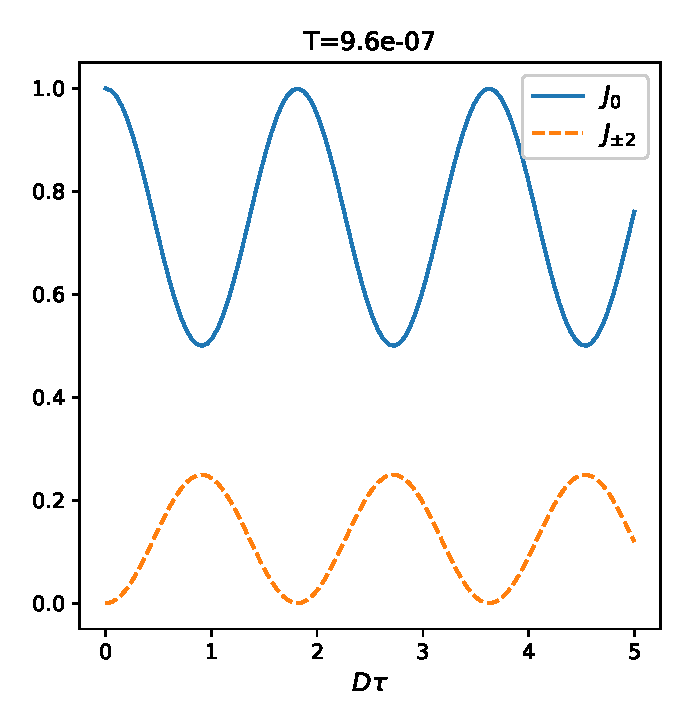
\includegraphics[width=0.5\linewidth]{coherences_n3_beta5.eps}
	\caption{
	  Интенсивности МК~когерентностей~ЯМР~$J_{n}$ ($n=0, 2$) в нанопоре с $N=3$.
      Здесь предполагается, что $\omega_{0} = 2\pi \cdot 500 \cdot 10^{6}$~s$^{-1}$ и $D = 2\pi \cdot 10^{4}$~s$^{-1}$.
	}
	\label{fig:1}
\end{figure}

В этом разделе будет получено точное решение МК~динамики~ЯМР~трехспиновой системы в дипольном упорядоченном состоянии в нанопоре.
Решение будет получена в общем виде, без использования высокотемпературного приближения~\cite{Goldman1970}.
Данная задача аналогична задаче, рассмотренной в разделе~\ref{sec:nanopora-thermodynamic-equilibrium}
для начального термодинамического равновесия в сильном внешнем магнитном поле.

Гамильтониан $H_{MQ}$ уравнения~(\ref{eq:hmq}) состоит из двух блоков для двух возможных значений углового момента спина $(I^2 = S(S+1), \quad S=3/2,1/2)$.
Эти блоки и соответствующие им собственные значения и собственные состояния приведены
в разделе~\ref{sec:sec:nanopora-thermodynamic-equilibrium-exact_sol}.
Матрица плотности системы также состоит из двух блоков $\rho^{3/2}(\tau)$, $\rho^{1/2}(\tau)$, и
%
\begin{equation}
  \label{eq:15}
  \rho^{3/2}(0) = \dfrac 1 Z
  \begin{pmatrix}
    e^{\frac{3b}{2}} & 0 & 0 & 0
    \\
    0 & e^{\frac{-3b}{2}} & 0 & 0
    \\
    0 & 0 & e^{\frac{-3b}{2}} & 0
    \\
    0 & 0 & 0 & e^{\frac{3b}{2}}
  \end{pmatrix},
  \quad
  \rho^{1/2}(0) = \dfrac 1 Z
  \begin{pmatrix}
    	1 & 0
    \\
    0 & 1
  \end{pmatrix}
\end{equation}
%
где $b = \dfrac{\hslash D}{k\mathrm{T}}$ и $T$ --- температура.
Простыми вычислениями можно получить матрицы плотности $\rho^{3/2}(\tau)$ и $\rho^{1/2}(\tau)$,
которые позволяют получить выражение для интенсивности МК~когерентностей~ЯМР.

В рассматриваемых системах появляются только МК~когерентности~ЯМР нулевого и плюс/минус второго порядков.
Интенсивности этих когерентностей равны
%
\begin{equation}
  \begin{split}
    \label{eq:16}
    J_0(\tau) & = 1
    - \dfrac 1 2 \tanh^2\left( \dfrac{3b}{2} \right)
      \sin^2 \left( \sqrt{3} Dt \right),
    \\
    J_{\pm2}(\tau) & = \dfrac{1}{4}
      \tanh^2 \left( \dfrac{3b}{2} \right)
      \sin^2 \left( \sqrt{3} Dt \right)
  \end{split}
\end{equation}
%
Сумма интенсивностей МК когерентностей согласно~(\ref{eq:16}) равна единице в соответствии с уравнением~(\ref{eq:14}).
Зависимости рассчитанных интенсивностей $J_{n}(\tau)$ $(n=0,2)$ от времени эволюции показаны на рисунке~(\ref{fig:1}).

% \subsection{Численный анализ многоспиновой запутанности при различных температурах и различном числе спинов в системе}
\subsection{Температурная зависимость многочастичной запутанности}
\label{sec:5}

В этом разделе приведены результаты полуаналитической симуляции МК эксперимента ЯМР
для модели спин-несущих молекул (атомов) в нанопоре в дипольном упорядоченном состоянии.
Будет рассмотрена зависимость нижней границы квантовой информации Фишера от времени и температуры.
А также получены оценки количества запутанных частиц в системе.
В расчетах предполагается, что $\omega_{0} = 2\pi \cdot 500 \cdot 10^{6}$~s$^{-1}$ и $D = 2\pi \cdot 10^{4}$~s$^{-1}$.

\begin{figure}[H]
 	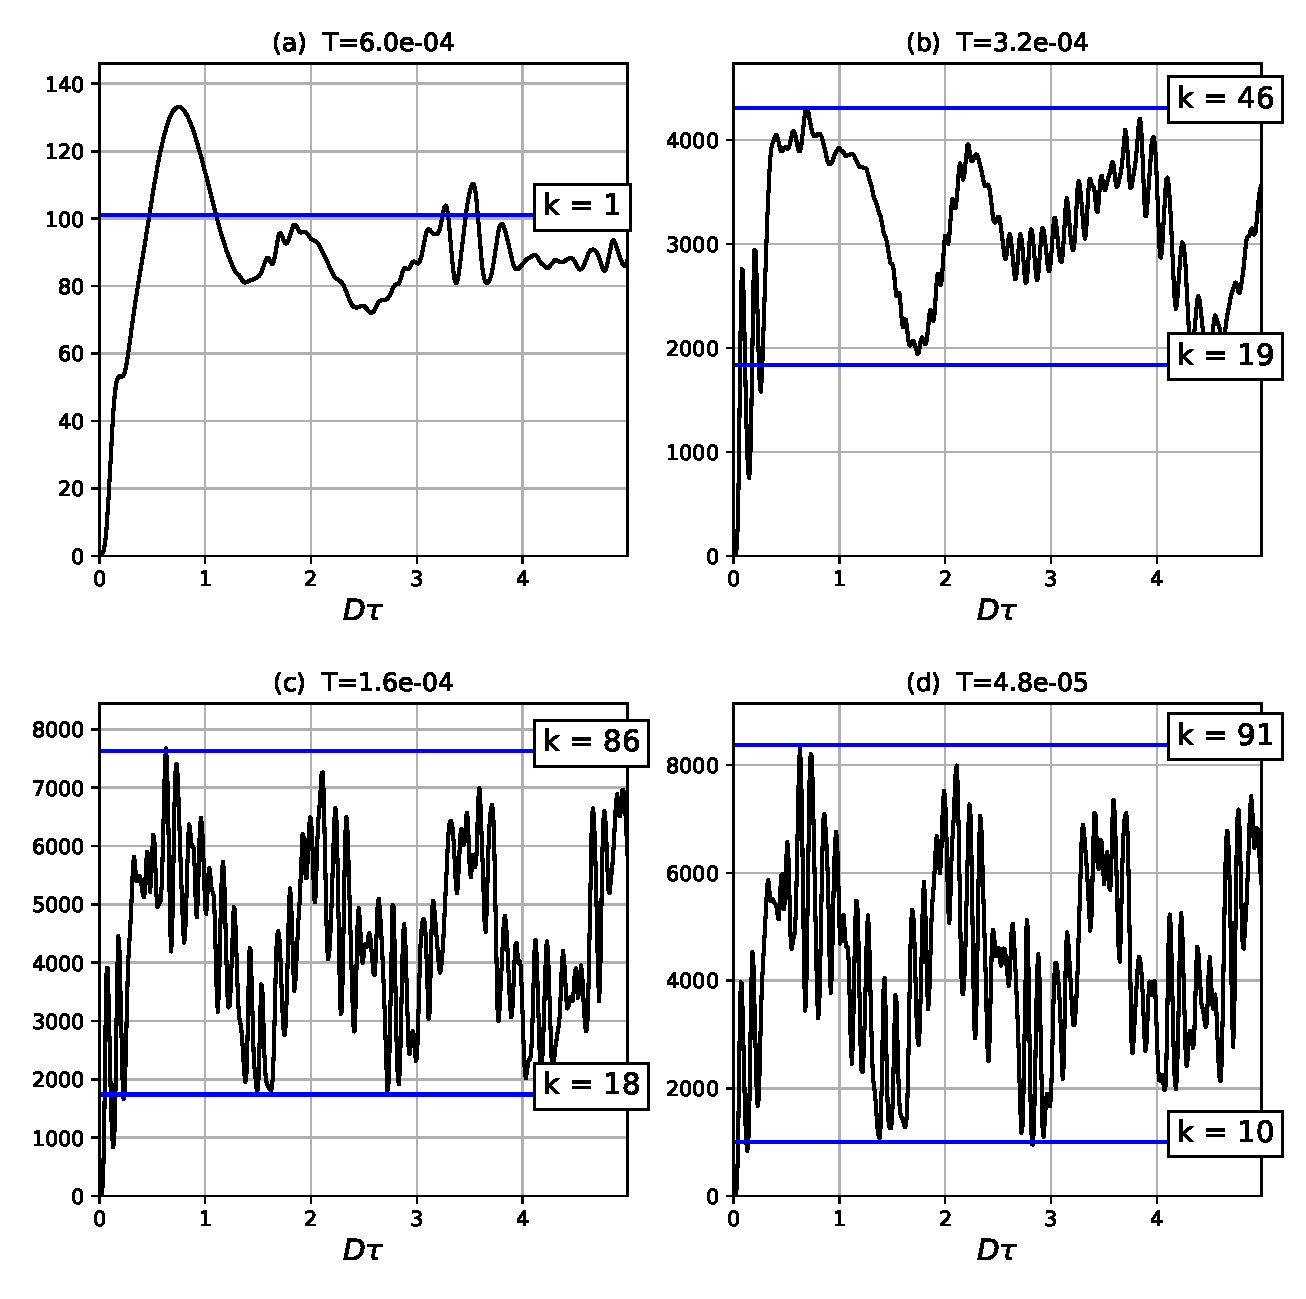
\includegraphics[width=0.95\linewidth]{fisher_low_bound_n101.eps}
	\caption{
	  Зависимость нижней границы  квантовой информации Фишера $F_\mathrm{Q} = 2 M_{2}$
	  от безразмерного времени $D\tau$ при $N=101$.
	  a) $T=6\cdot10^{-4}$~K, неравенство~(\ref{eq:20}) определяет область парной запутанности  (k+1=2), эта область выше горизонтальной линии;
	  b) $T=3.2\cdot10^{-4}$~K, область многоспиновой запутанности представляет собой полосу, ограниченную горизонтальными линиями с~$k=19$~и~$k=46$;
	  c) $T = 1.6\cdot10^{_4}$~K, горизонтальные линии ($k=18$ и $k=86$) ограничивают полосу с многоспиновой запутанностью;
	  d) при $T=4.8\cdot10^{-5}$~K возникают запутанные кластеры с $11-92$ спинами.
	}
	\label{fig:2}
\end{figure}


Рассматриваемая модель спин-несущих молекул (атомов) в нанопоре в дипольном упорядоченном состоянии
расширяет возможности исследования многоспиновой запутанности по сравнению с родственной моделью~(см. раздел~\ref{sec:nanopora-thermodynamic-equilibrium}),
в которой система изначально находилась в термодинамическом равновесии в сильном внешнем магнитном поле.
Модель из раздела~\ref{sec:nanopora-thermodynamic-equilibrium}) неприменима для исследования эволюции системы во времени,
потому что распределение МК~когерентностей~ЯМР~быстро становится стационарным~\cite{Doronin2009}.
Также многоспиновая запутанность изменяется с температурой в очень узком температурном интервале.
Например, все спины запутаны в системе, состоящей из 201 спина уже при температуре $T=6.856\cdot10^{-3}$~K~\cite{Doronin2019}.

Зависимость нижней границы квантовой информации Фишера от времени в системе, состоящей из 101 спина, представлена на Рис.~(\ref{fig:2}) при различных температурах.
Из Рис.~(\ref{fig:2}a) видно, что при температуре $T=6\cdot10^{-4}$~K существует только парная запутанность.
При температуре $T=3.2\cdot10^{-4}$ на Рис.~(\ref{fig:2}b) появляется полоса, в которой неравенство~(\ref{eq:entanglement-criteria}) может быть выполнено, когда $19 \leq k \leq 46$.
Таким образом, существует многоспиновая запутанность в спиновых кластерах, состоящих из 20-47 спинов, при температуре $3.2\cdot10^{-4}$~K.
Когда температура понижается, ширина полосы, в которой существует многоспиновая запутанность, увеличивается.
При температуре $T=1.6\cdot10^{-4}$~K (Рис.~(\ref{fig:2}c)) появляются кластеры из 19-87 запутанных спинов, а при температуре $T=4.8\cdot10^{-5}$~K (Рис.~(\ref{fig:2}d)), наблюдаются 11-92 запутанных спина.

\begin{figure}
 	\includegraphics[width=0.95\linewidth]{entangled_spins_by_n.eps}
	\caption{
	  Зависимость максимального количества запутанных спинов,
	  усредненного по времени эволюции $(0 \leq D\tau \leq 3)$,
	  от температуры при  a) $N=51$; b) $N=75$; c) $N=101$.
	}
	\label{fig:3}
\end{figure}

Зависимость максимального числа запутанных спинов за время эволюции $({0}\leq \mathrm{D}\tau\leq{3})$ от температуры при разных числах спинов в нанопоре представлена на Рис.~(\ref{fig:3}).
Максимальное количество запутанных спинов уменьшается при повышении температуры.
Максимальное количество запутанных спинов увеличивается, когда увеличивается число спинов в нанопоре, потому что система в нанопоре становится плотнее.

\section{Выводы}
\label{sec:conslusions}
% We investigated many-particle entanglement in MQ NMR spectroscopy using a nanocavity filled with spin-carrying atoms (molecules).
% We developed a theory of MQ NMR in a nanocavity at low temperatures.
% The theory is based on the idea that  molecular diffusion is substantially faster than the time of the spin flip-flop processes.
% As a result, the problem is reduced to a system of equivalent spins [23, 25], which can be analyzed in the basis of the common eigenstates of the total spin angular momentum and its projection on the external magnetic field.
% Since there is a connection between the second moment (dispersion) of the distribution of the MQ NMR intensities and many-spin entanglement [17], we extracted information about many-spin entanglement from the MQ NMR spectrum. The temperature dependence of many-spin entanglement was also investigated.
% \par
% The main lesson consists in significant growth of many-particle entanglement at low temperatures.
% All or almost all spins are entangled at the dimensionless temperature $\frac{1}{b}$ of the order of 1.
% This suggests that $k$-entangled states with large $k$ emerge in a typical MQ NMR system at low temperatures.
% This is particularly interesting given the absence of entanglement in the initial state. We expect such behavior to be typical for MQ NMR.
% \par
% We can conclude that MQ NMR spectroscopy is an effective method for the investigation of many-spin entanglement and the spreading of MQ correlations inside many-spin systems. It can be used for experimental investigations of quantum information processing in solids (note a related study of decoherence in liquids \cite{HOU2017863}).
% \par

В этой главе была исследована многочастичная запутанность в МК спектроскопии ЯМР в нанопоре, заполненной сотнями спин-несущими частицами.
Для этого была разработана МК теория ЯМР в нанопоре при низких температурах.
Было рассмотрено два начальных состояния системы:
термодинамически равновесное
и дипольное упорядоченное.
В обоих случах впервые удалось исследовать температурную зависимость многочастичной запутанности.
Все или почти все спины запутаны при безразмерной температуре $\frac{1}{b}$ порядка 1.
Это говорит о том, что $k$-запутанные состояния с большим $k$ возникают в типичной системе МК ЯМР при низких температурах.
Это особенно интересно, учитывая отсутствие запутанности в начальном состоянии.
Можно заключить, что такое поведение типично для МК ЯМР.
Так же была исследована зависимость многоспиновой запутанности
от количества спинов в нанопоре.
Показано, что с ростом количества спинов в нанопоре,
скорость возникновения запутанных кластеров при понижении температуры увеличивается.

Результаты этого раздела наглядно демонстрируют
универсальность разработанного в этой диссертации метода исследования многочастичной запутанности.

\begin{frame}{Эволюция нижней границы информации Фишера}
% (AMR-20)\footnote{G.A. Bochkin et al., \textit{Appl. Magn. Res.} \textbf{51}, 667-678, (2020)}
\begin{columns}

    \column{0.6\textwidth}
    \begin{figure}
    
\includegraphics[width=0.95\textwidth]{result-zchain-m2-by-time-n6-beta10.eps}
    %\caption{Hанопора со спин-несущих молекулами во внешнем сильном магнитном поле $\vec B$}
    \end{figure}

    \column{0.4\textwidth}
    Зависимость нижней границы квантовой информации Фишера
    $$ F_Q = 2M_2(\tau, T) $$
    от безразмерного времени $D_1 \tau$
    для шести спинов
    при температуре $T = 2.5 \times 10^{-3}$ $(\beta = 10)$.
    Область многочастичной запутанности ограничена горизонтальными линиями $k = 1$, $k = 5$.
\end{columns}
\end{frame}
\note{
   Мы не можем точно сказать сколько спинов запутанно,
   но можем дать нижнюю оценку на количество запутанных между собой спинов.
}


\begin{frame}{Максимальное количество запутанных спинов}
\begin{columns}

    \column{0.5\textwidth}
    \begin{figure}
    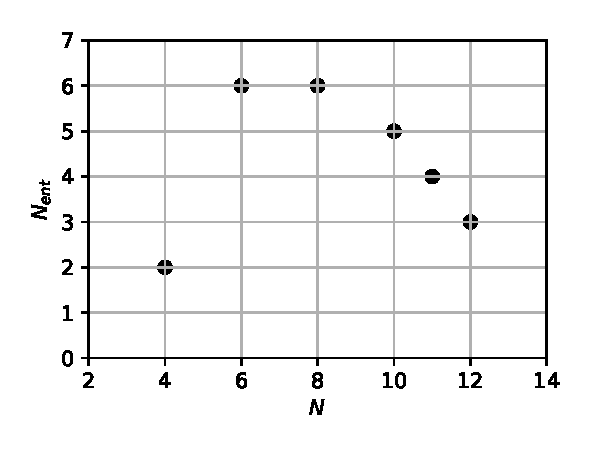
\includegraphics[width=\textwidth]{result-zchain-nent-by-n-beta10.eps}
    \caption{}
    \end{figure}

    \column{0.5\textwidth}
    Зависимость максимального количества запутанных спинов $N_\mathrm{ent}$ от длины цепи при температуре $T = 2.5 \times 10^{-3}$ $(\beta = 10)$.

    \vspace{0.5cm}

    \alert{Создание запутанных кластеров в рассматриваемых зигзагообразных цепочках ограничено слабыми дипольными взаимодействиями удаленных спинов}.
\end{columns}
\end{frame}
\note{
  Установлено что, при фиксированной температуре с ростом числа спинов в цепи размер запутанных кластеров может уменьшаться;
}


\begin{frame}{Максимальное количество запутанных спинов}
  \begin{columns}
     \column{0.5\textwidth}
     \begin{figure}
     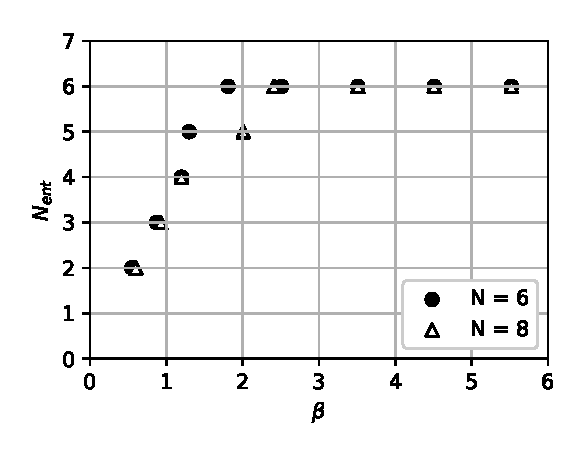
\includegraphics[width=\textwidth]{result-zchain-nent-by-beta-n8-n6.eps}
     \caption{}
     \end{figure}

     \column{0.45\textwidth}
     \begin{block}{}
       Зависимость максимального количества запутанных спинов $N_\mathrm{ent}$ от обратной температуры
       $$ \beta = \dfrac{\hbar\omega_0}{kT} $$
       в зигзагообразной цепочки из 6 и 8 спинов.
    \end{block}
  \end{columns}
\end{frame}
\note{
    Для 6 спинов накачка происходит быстрее, чем для 8 спинов.
}

\chapter{Измерение информации Вигнера-Янасе в МК эксперименте ЯМР}
\label{chapter:wyi-mesuarement}

% PLA-2021
\item
Разработана теория МК ЯМР в системе эквивалентных спинов s=1/2 при произвольных температурах. При низких температурах эта теория применена для расчетов многоспиновой запутанности в
нанопоре и зигзагообразной цепочке. 
Проведенные исследования позволяют заключить, что МК-спектроскопия ЯМР является тонким и полезным методом для исследования различных проблем квантовой информатики.

\item
Исследована температурная зависимость многочастичной запутанности в нанопоре с термодинамическим равновесным зеемановским и дипольно упорядоченным начальными состояниями. 
С понижением температуры количество запутанных спинов растет.
При температуре
$T = 6.856\cdot10^{-3}$~K $(\beta=3.5)$
почти все спины (до 179 из 201) запутаны. 
Можно заключить, что в типичной системе МК ЯМР при низких температурах возникают многочастичные запутанные состояния,
даже при отсутствии запутанности в начальном состоянии.  


\item
Исследована многочастичная запутанность в квазиодномерных цепочках ядерных спинов в зависимости от параметров цепи и температуры.
В однородных цепочках детектируется только парная запутанность, что согласуется с результатами, представленными в литературе.
В зигзагообразной цепочке при низких температурах почти все спины запутанны, так же как и в нанопоре.

\item
Предложен метод экспериментального измерения точного значения косой информации Вигнера-Янасе в рамках МК спектроскопии ЯМР.
Разработанный метод позволяет не только исследовать многочастичную запутанность методами МК ЯМР,
но и открывает возможность решения широкого класса задач квантовой теории информации.


\begin{thebibliography}{}

\bibitem{Einstein1935} A. Einstein, B. Podolsky, and N. Rosen \textit{Phys. Rev.} \textbf{47}, 777 (1935)
\bibitem{Bell1964} J.S. Bell \textit{Physics Physique Fizika} \textbf{1}, 195 (1964)
\bibitem{Scheidl2010} T. Scheidl et al. \textit{PNAS} \textbf{107}, 46, 19708-19713 (2010)

\bibitem{Bernabeu2012} Bernabéu, J., Martínez-Vidal, F. and Villanueva-Pérez, P. J. High Energ. Phys. 2012, 64 (2012).

\bibitem{Alain1976} Alain Aspect Phys. Rev. D 14, 1944 – Published 15 October 1976

% Zeqian Chen Phys. Rev. A 71, 052302
\bibitem{Gisin1991} N. Gisin, Phys. Lett. A 154, 201 (1991).
\bibitem{Clauser1969} J. F. Clauser, M. A. Horne, A. Shimony, and R. A. Holt, Phys. Rev. Lett. 23, 880 (1969).
\bibitem{Seevinck2002} M. Seevinck and G. Svetlichny, ibid. 89, 060401 (2002).
\bibitem{Uffink2002}  J. Uffink, Phys. Rev. Lett. 88, 230406 (2002O); K. Nagata, M. Koashi, and N. Imoto, ibid. 89, 260401 (2002).
%

\bibitem{Bennett1996} C.H.Bennett et al. \textit{Phys. Rev. A} \textbf{54}, 3824 (1996)
\bibitem{Eisert2001} Eisert J. and Briegel H. J. \textit{Phys. Rev. A} \textbf{64}, 022306 (2001)
\bibitem{Wootters1998} W.K. Wootters, \textit{Phys. Rev. Lett.} \textbf{80}, 2245 (1998)


% [5 - 31] P. Hyllus et al. Phys. Rev. A 85, 022321 (2012)
\bibitem{Plenio2007} M.B. Plenio and S. Virmani, Quant. Inf. Comp. 7, 1 (2007).
\bibitem{Amico2008} L. Amico, R. Fazio, A. Osterloh, and V. Vedral, Rev. Mod. Phys. 80, 517 (2008).
\bibitem{Horodecki2009} R. Horodecki, P. Horodecki, M. Horodecki, and K. Horodecki, Rev. Mod. Phys. 81, 865 (2009).
\bibitem{Guhne2009} O. G\"uhne and G. Toth, Physics Reports 474, 1 (2009).
\bibitem{Bourennane2004} M. Bourennane, M. Eibl, C. Kurtsiefer, S. Gaertner, H. Weinfurter, O. G\"uhne, P. Hyllus, D. Bruß, M. Lewenstein, and A. Sanpera, Phys. Rev. Lett. 92, 087902
\bibitem{Kaszlikowski2008} D. Kaszlikowski and A. Kay, New. J. Phys. 10, 053026 (2008).
\bibitem{Krammer2009} P. Krammer, H. Kampermann, D. Bruß, R.A. Bertlmann, L.C. Kwek, C. Macchiavello, Phys. Rev. Lett. 103, 100502 (2009).
\bibitem{Bancal2011} J.-D. Bancal, N. Gisin, Y.-C. Liang, and S. Pironio, PRL 106, 250404 (2011).
\bibitem{Svetlichny1987} G. Svetlichny, Phys. Rev. D 35, 3066 (1987).
\bibitem{Gisin1998} N. Gisin and H. Bechmann-Pasquinucci, Phys. Lett. A 246, 1 (1998).
\bibitem{Collins2002} D. Collins, N. Gisin, S. Popescu, D. Roberts, and V. Scarani, Phys. Rev. Lett. 88, 170405 (2002).
\bibitem{Seevinck2001} M. Seevinck and J. Uffink, Phys. Rev. A 65, 012107 (2001);
\bibitem{Toth2005} G. T\'oth, O. G\"uhne, M. Seevinck, and J. Uffink, Phys. Rev. A 72, 014101 (2005).
\bibitem{Nagata2002} K. Nagata, M. Koashi, and N. Imoto, Phys. Rev. Lett. 89, 260401 (2002).
\bibitem{Yu2003} S. Yu, Z.-B. Chen, J.-W. Pan, and Y.-D. Zhang, Phys. Rev. Lett. 90, 080401 (2003)
\bibitem{Laskowski2005} W.Laskowski and M.Zukowski, Phys.Rev.A72, 062112 (2005).
\bibitem{Schmid2008} C. Schmid, N. Kiesel, W. Laskowski, W. Wieczorek, and M.Z\'ukowski,and H.Weinfurter,Phys.Rev.Lett.100, 200407 (2008).
\bibitem{Bancal2009} J.-D. Bancal, C. Branciard, N. Gisin, and S. Pironio, Phys. Rev. Lett. 103, 090503 (2009).
\bibitem{Sorensen2001} A.S. Sørensen and K. Mølmer, Phys. Rev. Lett. 86, 4431 (2001).
\bibitem{Durkin2005} G.A. Durkin and C. Simon, Phys. Rev. Lett. 95, 180402 (2005).
\bibitem{Vitagliano2011} G. Vitagliano, P. Hyllus, I.L. Egusquiza, G. T\'oth, Phys. Rev. Lett. 107, 240502 (2011).
\bibitem{Duan2011} L.-M. Duan, Phys. Rev. Lett. 107, 180502 (2011).
\bibitem{Guhne2010} O. Guhne and M. Seevinck, New J. Phys. 12, 053002 (2010).
\bibitem{Huber2010} M. Huber, F. Mintert, A. Gabriel, and B.C. Hiesmayr, Phys. Rev. Lett. 104, 210501 (2010).
\bibitem{Li2010} C.-M. Li, K. Chen, A. Reingruber, Y.N. Chen, and J.W. Pan, Phys. Rev. Lett. 105, 210504 (2010).
\bibitem{Jungnitsch2011} B. Jungnitsch, T. Moroder, and O. G\"uhne, Phys. Rev. Lett. 106, 190502 (2011).
\bibitem{Vicente2011} J.I. de Vicente and M. Huber, Phys. Rev. A 84, 062306 (2011).
\bibitem{Huber2011} M. Huber, P. Erker, H. Schimpf, A. Gabriel, and B. Hiesmayr, Phys. Rev. A 83, 040301(R) (2011).
%---


\bibitem{Zeqian2005} Zeqian Chen \textit{Phys. Rev. A} \textbf{71}, 052302 (2005)

\bibitem{Hyllus2012} P. Hyllus et al. \textit{Phys. Rev. A} \textbf{85}, 022321 (2012)


% [19] Phys. Rev. A 71, 052302 (2005)
\bibitem{Wheeler2004} J.Wheeler, in Complexity, Entropy, and Physics of Information, edited by Z.H.Zurek (Addison-Wesley, Reading, MA, 1990), pp.3-28;
\bibitem{Summhammer2004}
J.Summhammer, Int.J.Theor.Phys. 33, 171(1994);
\bibitem{Frieden2004} B.R.Frieden, Science from Fisher Information: A Unification(Cambridge University Press, Cambridge, England, 2004).

\bibitem{khitrin1997} A. Khitrin, Chem. Phys. Lett. 274, 217 (1997)

\bibitem{g_arttner2018} M. G\"arttner, P. Hauke, and A. M. Rey, Phys. Rev. Lett. 120, 040402 (2018)

\bibitem{t_oth2014} G. T\"oth and I. Apellaniz, J. Phys. A 47, 424006 (2014)

\bibitem{pezz_e2018} L. Pezz\'e, A. Smerzi, M. K. Oberthaler et al., Rev. Mod. Phys. 90, 035005 (2018).

\bibitem{liu2014} J. Liu, H.-N. Xiong, F. Song, and X. Wang, Physica A 410, 167 (20


% Quatntum Fisher Information
\bibitem{Helstrom1976} C. W. Helstrom, Quantum detection and estimation theory, Academic Press, New York, 1976.
\bibitem{Holevo1982} A. S. Holevo, Probabilistic and statistical aspects of quantum theory, North-Holland, Amsterdam, 1982.


% Wigner yanase

% 10.1103/PhysRevLett.91.180403
% [3]
\bibitem{Araki1961} H. Araki and M. M. Yanase, Phys. Rev. 120, 622 (1960). [4] M. M. Yanase, Phys. Rev. 123, 666 (1961).
% [5]
\bibitem{Ozawa1991} M. Ozawa, Phys. Rev. Lett. 67, 1956 (1991).
% [6]
\bibitem{Ozawa2002a} M. Ozawa, Phys. Rev. Lett. 88, 050402 (2002).
% [7]
\bibitem{Ozawa2002b} M. Ozawa, Phys. Rev. Lett. 89, 057902 (2002).
% [8]
\bibitem{Matsumoto1993} S. Matsumoto, Prog. Theor. Phys. 90, 35 (1993).
% [9]
\bibitem{Kakazu3469} K. Kakazu and S. Pascazio, Phys. Rev. A 51, 3469
(1995).

% Chen2005
% 10.1103/PhysRevA.71.052302
% 3
% \bibitem{Einstein1935} A. Einstein, B. Podolsky, and N. Rosen, Phys. Rev. 47, 777 (1935).
% % 4
% \bibitem{Gisin1991} N. Gisin, Phys. Lett. A 154, 201 (1991).
% % 5
% \bibitem{Clauser1969} J. F. Clauser, M. A. Horne, A. Shimony, and R. A. Holt, Phys. Rev. Lett. 23, 880 (1969).
% ��6�� D. Collins, N. Gisin, S. Popescu, D. Roberts, and V. Scarani,
% Phys. Rev. Lett. 88, 170405 ��2002��; M. Seevinck and G.
% Svetlichny, ibid. 89, 060401 ��2002��.
% ��7�� J. Uffink, Phys. Rev. Lett. 88, 230406 ��2002��; K. Nagata, M.
% Koashi, and N. Imoto, ibid. 89, 260401 ��2002��.
% ��8�� S.-X. Yu, Z.-B. Chen, J.-W. Pan, and Y.-D. Zhang, Phys. Rev.
% Lett. 90, 080401 ��2003��.
% ��9�� E. P. Wigner, Z. Phys. 133, 101 ��1952��; Physikertagung Wien
% ��Physik-Verlag, Mosbach, 1952��, p. 1.

% E. P. Wigner and M. M. Yanase, \textit{Proc. Nat. Acad. Sci. USA}, \textbf{49}, 910–918 (1963)
% [1]
\bibitem{Weaver1949} W. Weaver's article in The Mathematical Theory of Communication (Urbana: The University of IllinoisPress,1949),p.45. SeealsothelastfewpagesofM.v.Smoluchowski'sarticleinVortrage fiberdie kinetische Theorie der Materie und Elektrizit4t (Leipzig: B. G. Teubner, 1914).
% [2]
\bibitem{Wigner1960} Wigner, E. P., Z. Physik, 131, 101 (1952); Araki, H., and M. M. Yanase, Phys. Rev., 120, 622(1960).
% [3]
\bibitem{Wigner1962} Wigner,E.P.,PhysikertagungWien(Mosbach/Baden: PhysikVerlag,1962),p.1

\bibitem{Wigner1963} E. P. Wigner and M. M. Yanase, \textit{Proc. Nat. Acad. Sci. USA}, \textbf{49}, 910–918 (1963) https://www.pnas.org/doi/abs/10.1073/pnas.49.6.910

\bibitem{Luo2003} S. Luo, \textit{Phys. Rev. Lett.} \textbf{91}, 180403 (2003)

\bibitem{Lieb1973prl} E. H. Lieb and M. B. Ruskai, “A fundamental property of quantum-mechanical entropy,” Phys. Rev. Lett., 30, 434–436 (1973).
\bibitem{Lieb1973} E. H. Lieb, “Convex trace functions and the Wigner–Yanase–Dyson conjecture,” Adv. Math., 11, 267–288 (1973).
\bibitem{Wehrl1978} A. Wehrl, “General properties of entropy,” Rev. Modern Phys., 50, 221–260 (1978).

\bibitem{Luo2005} S. L. Luo, “Quantum versus classical uncertainty,” Theor. Math. Phys., 143, 681–688 (2005).
\bibitem{Luo2005pra} S. Luo, “Heisenberg uncertainty relation for mixed states,” Phys. Rev. A, 72, 042110 (2005).
\bibitem{Luo2006} S. Luo, “Quantum uncertainty of mixed states based on skew information,” Phys. Rev. A, 73, 022324 (2006).
\bibitem{Luo2017pra} S. Luo and Y. Sun, “Quantum coherence versus quantum uncertainty,” Phys. Rev. A, 96, 022130 (2017).

\bibitem{Luo2020} S. Luo, Theoretical and Mathematical Physics, 202(1): 104–111 (2020)
% [9-23] Luo, Theoretical and Mathematical Physics, 202(1): 104–111 (2020)
% 9.
\bibitem{Luo2012} S. Luo, S. Fu, and C. H. Oh, “Quantifying correlations via the Wigner–Yanase skew information,” Phys. Rev. A,
85, 032117 (2012).
%10.
\bibitem{Li2016a} L. Li, Q.-W. Wang, S.-Q. Shen, and M. Li, “Measurement-induced nonlocality based on Wigner–Yanase skew
information,” Europhys. Lett., 114, 10007 (2016).
%11.
\bibitem{Sun2017} Y. Sun, Y. Mao, and S. Luo, “From quantum coherence to quantum correlations,” Europhys. Lett., 118, 60007
(2017).
% 12.
\bibitem{Girolami2014} D. Girolami, “Observable measure of quantum coherence in finite dimensional systems,” Phys. Rev. Lett., 113,
170401 (2014); arXiv:1403.2446v3 [quant-ph] (2014).
% 13.
\bibitem{Yu2017} C. Yu, “Quantum coherence via skew information and its polygamy,” Phys. Rev. A, 95, 042337 (2017); arXiv:
1704.04871v1 [quant-ph] (2017).
% 14.
\bibitem{Luo2017} S. Luo and Y. Sun, “Partial coherence with application to the monotonicity problem of coherence involving skew
information,” Phys. Rev. A, 96, 022136 (2017).
% 15.
\bibitem{Luo2018} S. Luo and Y. Sun, “Coherence and complementarity in state-channel interaction,” Phys. Rev. A, 98, 012113
(2018).
% 16.
\bibitem{Karpat2014} G. Karpat, B. Cakmak, and F. F. Fanchini, “Quantum coherence and uncertainty in the anisotropic XY chain,”
Phys. Rev. B, 90, 104431 (2014); arXiv:1404.6427v3 [quant-ph] (2014).
% 17.
\bibitem{Malvezzi2016} A. L. Malvezzi, G. Karpat, B. Cakmak, F. F. Fanchini, T. Debarba, and R. O. Vianna, “Quantum correlations
and coherence in spin-1 Heisenberg chains,” Phys. Rev. B, 93, 184428 (2016); arXiv:1602.03731v2 [quant-ph]
(2016).
% 18.
\bibitem{Li2016b} Y.-C. Li and H.-Q. Lin, “Quantum coherence and quantum phase transitions,” Sci. Rep., 6, 26365 (2016).
% 19.
\bibitem{Lei2016} S. Lei and P. Tong, “Wigner–Yanase skew information and quantum phase transition in one-dimensional quantum spin-1/2 chains,” Quantum Inf. Process., 15, 1811–1825 (2016).
% 20.
\bibitem{Qiu2017} L. Qiu, D. Quan, F. Pan, and Z. Liu, “Skew information in the XY model with staggered Dzyaloshinskii–Moriya
interaction,” Phys. B, 514, 13–18 (2017).
% 21.
\bibitem{Yanagi2005} K. Yanagi, S. Furuichi, and K. Kuriyama, “A generalized skew information and uncertainty relation,” IEEE Trans. Inform. Theory, 51, 4401–4404 (2005).
% 22.
\bibitem{Furuichi2010} S. Furuichi, “Schrodinger uncertainty relation with Wigner–Yanase skew information,” Phys. Rev. A, 82, 034101 (2010); arXiv:1005.2655v2 [quant-ph] (2010).
% 23.
\bibitem{Chen2016} B. Chen, S.-M. Fei, and G.-L. Long, “Sum uncertainty relations based on Wigner–Yanase skew information,” Quantum Inf. Process., 15, 2639–2648 (2016); arXiv:1606.01533v1 [quant-ph] (2016).
/Furuichi2010


% mq expreimetn
\bibitem{Baum1985} J. Baum, M. Munowitz, A. N. Garroway, and A. Pines, J. Chem. Phys. 83, 2015 (1985).


% models
\bibitem{Baugh2001}J. Baugh, A. Kleinhammes, D. Han, Q. Wang, and Y. Wu, \textit{Science} \textbf{294}, 1505 (2001).


% MQ NMR

%% Master diploma
\bibitem{vesta} Koichi Momma and Fujio Izumi. VESTA 3 for three-dimensional visualization of crystal, volumetric and morphology data. Journal of Applied Crystallography, 44(6):1272–1276, Dec 2011.

\bibitem{Elliott1994} J. C. Elliott. Structure and chemistry of the apatites and other calcium orthophosphates. Studies in Inorganic Chemistry 18. Elsevier Science, Amsterdam, 1994.

%% JETP Lett. 2015
%\bibitem{Baum1985} J. Baum, M. Munoviz, A. N. Garroway, and A. Pines. Multiple quantum dynamics in solid state NMR. The Journal of Chemical Physics, 83(5):2015– 2025, 1985.

%%
\bibitem{Bochkin2019jmr} G.A. Bochkin, E.B. Fel’dman, I.D. Lazarev, A.A. Samoilenko, S.G. Vasil’ev, Orientational dependencies of dynamics and relaxation of multiple quantum NMR coherences in one-dimensional systems, Journal of Magnetic Resonance (2019), doi: https://doi.org/10.1016/j.jmr.2019.02.004

%% JMR 2020
% []
% [1]
% \bibitem{Baum1985} J. Baum, M. Munowitz, A.N. Garroway, A. Pines, J. Chem. Phys. 83 (5) (1985) 2015–2025.
% [2]
\bibitem{Hughes2004} C.E. Hughes, Prog. Nucl. Magn. Reson. Spectrosc. 45 (3–4) (2004) 301–313.
% [3]
\bibitem{Vasilev2018} S.G. Vasil’ev, V.I. Volkov, E.A. Tatarinova, A.M. Muzafarov, N.A. Sipyagina, S.A. Lermontov, J. Non-Cryst. Solids 489 (2018) 6–15.
% [4]
\bibitem{Avilova2019} I.A. Avilova, A.V. Chernyak, S.G. Vasil’ev, Appl. Magn. Resonan. 50 (12) (2019) 1419 –1428.
% [5]
\bibitem{Mogami2014} Y. Mogami, S. Yamazaki, S. Matsuno, K. Matsui, Y. Noda, K. Takegoshi, Cem. Concr. Res. 66 (2014) 115–120.
% [6]
\bibitem{Krojanski2006} H.G. Krojanski, D. Suter, Phys. Rev. A 74 (6) (2006) 062319.
% [7]
\bibitem{Cho2006} H. Cho, P. Cappellaro, D.G. Cory, C. Ramanathan, Phys. Rev. B 74 (22) (2006) 224434.
% [8]
\bibitem{Bochkin2018} G.A. Bochkin, E.B. Fel’dman, S.G. Vasil’ev, V.I. Volkov, Appl. Magn. Reson. 49 (1) (2018) 25–34.
% [9]
\bibitem{Sanchez2014} C.M. S\'anchez, R.H. Acosta, P.R. Levstein, H.M. Pastawski, A.K. Chattah, Phys. Rev. A 90 (4) (2014) 042122.
% [10]
\bibitem{Alvarez2015} G.A. \'Alvarez, D. Suter, R. Kaiser, Science 349 (6250) (2015) 846–848.
% [11]
\bibitem{Wei2018} K.X. Wei, C. Ramanathan, P. Cappellaro, Phys. Rev. Lett. 120 (7) (2018) 070501.
% [12]
\bibitem{Garttner2018} M. G\"arttner, P. Hauke, A.M. Rey, Phys. Rev. Lett. 120 (4) (2018) 040402.
% [13]
\bibitem{Doronin2019} S.I. Doronin, E.B. Fel’dman, I.D. Lazarev, Phys. Rev. A 100 (2) (2019) 022330.
% [14]
\bibitem{Starkov2020}  G.A. Starkov, B.V. Fine, Phys. Rev. B 101 (2) (2020) 024428.
% [15]
\bibitem{Zhang2009} W. Zhang, P. Cappellaro, N. Antler, B. Pepper, D.G. Cory, V.V. Dobrovitski, C. Ramanathan, L. Viola, Phys. Rev. A 80 (5) (2009) 052323.
% [16]
\bibitem{Feldman2014} E.B. Fel’dman, Appl. Magn. Reson. 45 (8) (2014) 797–806.
% [17]
\bibitem{Feldman1997} E.B. Fel’dman, S. Lacelle, J. Chem. Phys. 107 (18) (1997) 7067–7084.
% [18]
\bibitem{Hayashi1960} S. Hayashi, Nippon kagaku zassi 81 (4) (1960) 540–542.
% [19]
\bibitem{Van1964} W. Van der Lugt, W.J. Caspers, Physica 30 (8) (1964) 1658–1666.
% [20]
\bibitem{ChoCho} G. Cho, J.P. Yesinowski, J. Phys. Chem. 100 (39) (Cho) 15716–15725.
% [21]
\bibitem{Itoh2005} K.M. Itoh, Solid State Commun. 133 (11) (2005) 747–752.
% [22]
\bibitem{Zachariasen1931} W.H. Zachariasen, Zeitschrift für Kristallographie - Crystalline Materials 76 (1) (1931) 289–302.
% [23]
\bibitem{Zachariasen1963} W.H. Zachariasen, H.A. Plettinger, M. Marezio, Acta Crystallogr. A 16 (11) (1963) 1144–1146.
% [24]
\bibitem{Gatta2012} G.D. Gatta, J.M. Garry, B. Geoffrey, G. Alessandro, N. Fabrizio, Am. Mineral. 97 (11–12) (2012) 1891–1897.
% [25]
\bibitem{Burns1995} P.C. Burns, M. Novak, F.C. Hawthorne, Can. Mineralogist 33 (6) (1995) 1205– 1213.
% [26]
\bibitem{Bochkin2019} G.A. Bochkin, E.B. Fel’dman, I.D. Lazarev, A.A. Samoilenko, S.G. Vasil’ev, J. Magn. Reson. 301 (2019) 10–18.
% [27]
\bibitem{Abragam1961} A. Abragam, The principles of nuclear magnetism, Clarendon Press, Oxford, 1961.
% [28]
\bibitem{Carolan1971} J.L. Carolan, Chem. Phys. Lett. 12 (2) (1971) 389–391.
% [29]
\bibitem{Vleck1948} J.H. Van Vleck, Phys. Rev. 74 (9) (1948) 1168–1183.
% [30]
\bibitem{Engelsberg1973} M. Engelsberg, I.J. Lowe, J.L. Carolan, Phys. Rev. B 7 (3) (1973) 924–929.
%% --


\end{thebibliography}


\end{document}
\begin{frame}{Определение информации Фишера в МК ЯМР (PRA-19)\footnote{S.I. Doronin, E.B. Fel'dman,  I.D. Lazarev, \textit{Phys. Rev. A}, \textbf{100}, 022330 (2019)}}
  $$ G(\tau, \phi) =
     \mathrm{Tr}\left\{
         e^{iH_\mathrm{MQ}\tau} e^{i\phi I_z} e^{-iH_\mathrm{MQ}\tau}
         \rho_\mathrm{eq}
         e^{iH_\mathrm{MQ}\tau} e^{-i\phi I_z} e^{-iH_\mathrm{MQ}\tau}
         I_z \right\}
  $$
  \begin{alertblock}{}
      Дисперсия распределения интенсивности МК когерентностей ЯМР определяет нижнюю границу информации
      Фишера\footnote[frame]{
      M. G\"arttner, P. Hauke, and A.M. Rey. \textit{Phys. Rev. Lett.} \textbf{120}, 040402 (2018)}:
      $$
      F_Q \geq 2M_2
      $$
  \end{alertblock}
  Однако формула справедлива только в том случае,
  если сигнал $G(\tau, \varphi)$ является \textit{out-of-time-ordered correlator} (OTOC).
  Для низких температур это условие не выполняется.
  Возможно обойти это ограничение,
  если усреднить сигнал МК эксперимента ЯМР по начальному состоянию:
  $$ G_\mathrm{LT}(\tau, \phi)
     = \mathrm{Tr}\left\{
       e^{iH_\mathrm{MQ}\tau} e^{i\phi I_z} e^{-iH_\mathrm{MQ}\tau}
       \rho_\mathrm{eq}
       e^{iH_\mathrm{MQ}\tau} e^{-i\phi I_z} e^{-iH_\mathrm{MQ}\tau}
       {\color{red} \rho_\mathrm{eq}}
    \right\}
  $$
\end{frame}



\chapter{Многоспиновая запутанность в системе эквивалентных спинов}
\label{chapter:manyparticle-entanglement-in-nanopore}
% \subsection{Создание дипольно упорядоченных состояний}
% (PRA-2019)
%   - Температурная зависимость многочастичной запутанности
%   - Зависимость от числа частиц
%
% Многоспиновая запутанность c дипольно упорядоченном начальном

% JETP-2020


Результат полученный в предыдущей главе~\ref{chapter:quantum-fisher-information-measurement}
позволяет в рамках МК динамики ЯМР прояснить более глубокие связи между MK когерентностями ЯМР и запутанностью.
Эти связи соответствуют распространению МК корреляций внутри многочастичной системы в процессе эволюции.
В результате из второго момента спектра интенсивности МК когерентностей ЯМР
можно извлечь информацию о многочастичной запутанности и свидетелях запутанности.

Для исследования многочастичной запутанности необходимо работать с моделью,
которая содержит достаточно большое ($>50$) количество взаимодействующих спинов,
и может быть экспериментально исследована при низких температурах.
Только тогда можно будет исследовать многочастичную запутанность и ее зависимость от температуры.
В разделе~\ref{sec:model-equivalent-spins} была рассмотрена несферическая нанопора,
заполненная газом со спин-несущими атомами (например, ксеноном) или молекулами в сильном внешнем магнитном поле.
Эта модель полностью отвечает поставленным требованиям.
По существу нанопора является системой эквивалентных спинов,
и ее МК динамика ЯМР может быть исследована точно.

На подготовительном периоде МК эксперимента ЯМР гамильтониан системы эквивалентных спинов
определяется выражением (см~\ref{sec:model-equivalent-spins})
\begin{equation}\label{eq:mq-hamiltoninan-equivalent-spins}
  H_\mathrm{MQ} = - \dfrac{D}{4} \left[
    \left( I^{+} \right)^2 + \left( I^{-} \right)^2
  \right],
  \quad
  I^{\pm} = \sum\limits_{j=1}^{N} I^{\pm}_j,
\end{equation}
где $I^{\pm}_{j}$ --- повышающий или понижающий операторы спина $j$,
$N$ --- число спинов в нанопоре,
$D$ - константа диполь-дипольного взаимодействия (ДДВ),
усредненная по быстрой молекулярной диффузии спин-несущих атомов (молекул) в нанопоре.
Как уже было обсуждено в разделе~\ref{sec:model-equivalent-spins},
гамильтониан $H_\mathrm{MQ}$
коммутирует с квадратом полного спинового углового момента $\hat I^2$,
поэтому удобно перейти к базису,
состоящего из общих собственных состояний $\hat I^2$ и $I_z$.
В этом базисе гамильтониан $H_{MQ}$ состоит из блоков $H_{MQ}^S$, соответствующих различным значениям полного спинового углового момента $S$:
\begin{equation}
  \hat I^2 = S(S+1), S = N/2, N/2-1, N/2-2,
\end{equation}
где
$N/2 - [N/2]$, $[i]$ - целая часть $i$.

Далее в этой главе будут рассмотрены два наиболее интересных начальных состояний системы
и исследованы температурные зависимости многоспиновой запутанности для каждого случая.

\section{Термодинамически равновесное начальное состояние}
\label{sec:nanopora-thermodynamic-equilibrium}

Для исследования многочастичной запутанности в зависимости от температуры,
в этом разделе будет рассмотрена МК динамика ЯМР
системы эквивалентных спинов размера $N$
с начальным термодинамически равновесным состоянием $\rho_\mathrm{eq}$:
%
\begin{equation}\label{eq:rho_eq}
  \rho(0) = \rho_{\mathrm{eq}} = \dfrac{e^{\frac{\hbar\omega_{0}}{kT} I_z}}{Z},
\end{equation}
%
где $Z =\mathrm{Tr}\left\{e^{\frac{\hbar\omega_{0}}{kT} I_z}\right\}$ это статистическая сумма,
$\hbar$ и $k$ --- это постоянная Планка и постоянная Больцмана,
$\omega_0$ --- Ларморовская частота,
$T$ --- температура,
и $I_z$ это оператор проекции полного углового момента на ось $z$,
которая направлена вдоль сильного внешнего магнитного поля.
%
Существующий теоретический подход~\cite{Doronin2009, Doronin2011}
к МК динамике ЯМР системы эквивалентных спинов
применим только в высокотемпературной области.
Для исследования многочастичной запутанности,
необходимо разработать теорию МК динамики ЯМР системы эквивалентных спинов
для произвольных температур,
что будет сделано ниже.
% Так же будут приведены вычисления для системы из 51, 75, 101, 201 спинов,
% но, в принципе, аналогичные расчеты можно провести и для систем с несколькими тысячами спинов.

Поскольку и гамильтониан $H_{MQ}$, и матрица начальной плотности из уравнения~(\ref{eq:rho_eq}) имеют блочную структуру,
можно заключить,
что эволюционная матрица плотности $\rho_\mathrm{LT}(\tau)$:
%
\begin{equation}
  \label{eq:rho_eval_lt}
  \rho_\mathrm{LT} (\tau) = e^{-iH_\mathrm{MQ}\tau} \rho_\mathrm{eq} e^{iH_\mathrm{MQ}\tau},
\end{equation}
%
также состоит из блоков $\rho^S_\mathrm{LT}(\tau)$,
где $(S=\frac N 2, \frac N 2 - 1, \dots, \frac N 2 - \left[\frac N 2\right])$.
Введем обозначение $\rho^S_{\mathrm{LT}, n}(\tau)$ для
вклада в $\rho^S_\mathrm{LT}(\tau)$ от МК когерентности ЯМР порядка $n$.
Тогда вклад $J_{\mathrm{LT}, n, S}(\tau)$ в интенсивность приведенной МК когерентности ЯМР $n$-го порядка определяется как
%
\begin{equation}
    \label{eq:coherence_k_s}
    J_{\mathrm{LT}, n, S}(\tau) = \dfrac{\mathrm{Tr}\left\{
        \rho_{LT, n}^S(\tau)\rho_{LT, -n}^S(\tau)
    \right\}}
    {\mathrm{Tr}\left\{\rho^2_{eq}\right\}}.
\end{equation}
%
Таким образом задача вычисления когерентностей сводится к вычислению отдельных вкладов для каждого значения полного углового момента $S$.

Наблюдаемые интенсивности приведенных МК когерентностей ЯМР рассчитываются по формуле:
%
\begin{equation}\label{eq:coherence_k}
  J_{\mathrm{LT}, n}(\tau) = \sum\limits_S n_N(S) J_{\mathrm{LT}, n, S}(\tau),
  \quad
  (-N\leq n \leq N),
\end{equation}
%
где $n_N(S)$ --- это кратность интенсивности $J_{n, S}(\tau)$,
определенная в разделе~\ref{sec:model-equivalent-spins} в~(\ref{eq:coeff_n}).


\subsection{Аналитическое решение для трехспиновой системы}
\label{sec:sec:nanopora-thermodynamic-equilibrium-exact_sol}

% \begin{figure}[H]
%   \centering
%   \includegraphics{exact_j.pdf}
%   \caption{Intensities of MQ NMR coherences $J_n, \quad n=0, 2$ in a nanopore with $N = 3$.}
%   \label{fig:exact_j}
% \end{figure}

В этом разделе будет рассмотрена система из $N=3$ спинов
связанных $H_{MQ}$ гамильтонианом,
определенном в выражении (\ref{eq:mq-hamiltoninan-equivalent-spins}).
Возможными значениями полного углового момента спина $S$
являются $\frac 3 2$ и $\frac 1 2$.
Ненулевые элементы блока гамильтониана $H_{MQ}^{S}$ определены в выражении~(\ref{eq:i-square-elements}).
Матричное представление $H_{MQ}^{3/2}$ имеет вид
%
\begin{equation}
    \label{eq:ham_3_2}
    H_{MQ}^{3/2} =
    \begin{pmatrix}
        0 & 0 & -\frac{\sqrt{3} D}{2} & 0 \\
        0 & 0 & 0 & -\frac{\sqrt{3} D}{2} \\
        -\frac{\sqrt{3} D}{2} & 0 & 0 & 0 \\
        0 & -\frac{\sqrt{3} D}{2} & 0 & 0
    \end{pmatrix}.
\end{equation}
%
Собственные значения $\lambda_{3/2}^{(i)}(i=1, 2, 3, 4)$
блока гамильтониана $H_{MQ}^{3/2}$ следующие
%
\begin{equation}\label{eq:eigvals_3_2}
  \lambda_{3/2}^{(1)} = -\frac{\sqrt{3} D}{2}, \quad
  \lambda_{3/2}^{(2)} = -\frac{\sqrt{3} D}{2}, \quad
  \lambda_{3/2}^{(3)} = \frac{\sqrt{3} D}{2}, \quad
  \lambda_{3/2}^{(4)} = \frac{\sqrt{3} D}{2}.
\end{equation}
%
Соответствующий набор собственных векторов выглядит следующим образом:
%
\begin{align}\label{eq:eigvecs_3_2}
  u_{3/2}^{(1)} & =  \left(\frac{1}{\sqrt{2}}, 0, \frac{1}{\sqrt{2}}, 0\right) ,
  \notag \\
  u_{3/2}^{(2)} & =  \left(0, \frac{1}{\sqrt{2}}, 0, \frac{1}{\sqrt{2}}\right) ,
  \notag \\
  u_{3/2}^{(3)} & =  \left(-\frac{1}{\sqrt{2}}, 0, \frac{1}{\sqrt{2}}, 0\right) ,
  \notag \\
  u_{3/2}^{(4)} & =  \left(0, -\frac{1}{\sqrt{2}}, 0, \frac{1}{\sqrt{2}}\right) .
\end{align}
%
Блок $H^{1/2}_{MQ}$ является скаляром
%
\begin{equation}\label{eq:ham_1_2}
  H^{1/2}_{MQ} = 0.
\end{equation}
%
Блоки эволюционной матрицы плотности $\rho_\mathrm{LT}^{n/2}(\tau) \quad (n = 1, 3)$
могут быть вычислены по формуле
%
\begin{equation}\label{eq:liouvile_sol}
  \rho_\mathrm{LT}^{n/2}(\tau) =
  U_{n/2} e^{-i\Lambda^{n/2}\tau} U^{+}_{n/2}
  \rho^{n/2}_\mathrm{LT}(0)
  U_{n/2} e^{i\Lambda^{n/2}\tau} U^{+}_{n/2},
\end{equation}
%
где $\Lambda^{n/2}$ --- диагональная матрица собственных значений,
$U_{n/2}$ --- матрица собственных векторов блока $H_{MQ}^{n/2} \quad (n=1, 3)$,
а начальная матрица плотности $\rho_\mathrm{LT}^{n/2}(0)$ имеет вид:
%
\begin{equation}\label{eq:rho_LT_init}
  \rho_\mathrm{LT}^{3/2}(0) = \dfrac 1 Z
  \begin{pmatrix}
      e^{\frac{3b}{2}} & 0 & 0 & 0
      \\
      0 & e^{\frac{b}{2}} & 0 & 0
      \\
      0 & 0 & e^{-\frac{b}{2}} & 0
      \\
      0 & 0 & 0 & e^{-\frac{3b}{2}}
  \end{pmatrix},
  \quad
  \rho_\mathrm{LT}^{1/2}(0) = \dfrac 1 Z
  \begin{pmatrix}
      e^{\frac{b}{2}} & 0
      \\
      0 & e^{-\frac{b}{2}}
  \end{pmatrix}.
\end{equation}
После вычисления выражений
(\ref{eq:eigvals_3_2}),
(\ref{eq:eigvecs_3_2}),
(\ref{eq:liouvile_sol})
и (\ref{eq:rho_LT_init}) с $n = 3$,
получаем
%
\begin{equation}\label{eq:rho_LT_eval_3_2}
  \rho_\mathrm{LT}^{3/2}(\tau) = \frac{1}{Z} \\
  \begin{pmatrix}
      ue^{-\frac{b}{2}} + ve^{\frac{3b}{2}}
    &
      0
    &
      -ie^{\frac{b}{2}}w
    &
      0
    \\
      0
    &
      ue^{-\frac{3b}{2}} + ve^{\frac{b}{2}}
    &
      0
    &
      -ie^{-\frac{b}{2}}w
    \\
      ie^{\frac{b}{2}}w
    &
      0
    &
      ue^{\frac{3b}{2}} + ve^{-\frac{b}{2}}
    &
      0
    \\
      0
    &
      ie^{-\frac{b}{2}}w
    &
      0
    &
      ue^{\frac{b}{2}} + ve^{-\frac{3b}{2}}
  \end{pmatrix},
\end{equation}
где
\begin{equation}
    u = \sin^2\left(\frac{\sqrt{3}}{2}D\tau\right),
    \quad
    v = \cos^2\left(\frac{\sqrt{3}}{2}D\tau\right),
    \quad
    w = \sin(b)\sin\left(\sqrt{3}D\tau\right).
\end{equation}
%
Аналогичные вычисления для матрицы $\rho^{1/2}_\mathrm{LT} (\tau)$
с использованием выражений (\ref{eq:liouvile_sol}) и (\ref{eq:rho_LT_init})
дают
%
\begin{equation}
\label{eq:rho_LT_eval_1_2}
    \rho_\mathrm{LT}^{1/2}(\tau) = \frac 1 Z
    \begin{pmatrix}
            e^{\frac b 2}
        &
            0
        \\
            0
        &
            e^{-\frac b 2}
    \end{pmatrix}.
\end{equation}

В рассматриваемой системе появляются только МК когерентности ЯМР нулевого и плюс/минус второго порядков.
Эти интенсивности могут быть вычислены с помощью выражений
(\ref{eq:coherence_k_s}), (\ref{eq:rho_LT_eval_3_2}) и (\ref{eq:rho_LT_eval_1_2})
%
\begin{align}\label{eq:j_lt_3}
  J_{\mathrm{LT}, 0}(\tau) & = 1 - \frac 1 2 \tanh^2(b)\sin^2(\sqrt 3 D \tau), \notag \\
  J_{\mathrm{LT},\pm 2}(\tau) & = \frac 1 4 \tanh^2(b)\sin^2(\sqrt 3 D \tau)
\end{align}
%
Можно убедиться что сумма интенсивностей~(\ref{eq:j_lt_3}) равна 1
и не зависит от времени $\tau$, так же как и в~(\ref{eq:sum_of_coherence}).
Профили рассчитанных интенсивностей $J_n(\mathrm{LT}, \tau)$, $(n=0,2)$ показаны на рис.~\ref{fig:exact_j}.


\subsection{Температурная зависимость многочастичной запутанности}
%\subsection{The temperature dependence of the many-particle entanglement}
\label{sec:entanglement}
В этом разделе приведены результаты полуаналитической симуляции МК эксперимента ЯМР
для модели спин-несущих молекул (атомов) в нанопоре в термодинамически равновесном состоянии.
Будет рассмотрена зависимость нижней границы квантовой информации Фишера от времени и температуры.
А также будут получены оценки количества запутанных частиц в системе,
состоящей из 201 спина.
% В расчетах предполагается, что $\omega_{0} = 2\pi \cdot 500 \cdot 10^{6}$~s$^{-1}$ и $D = 2\pi \cdot 10^{4}$~s$^{-1}$.

\begin{figure}[H]
  \centering
  \begin{subfigure}[t]{0.4\textwidth}
    %\centering
    \includegraphics[width=\textwidth]{m2_t_b01.pdf}
    \caption{
      ${T=2.4\cdot10^{-1}}$~K $(b=0.1)$.
      Парная запутанности выше горизонтальной линии.
      %The inequality~(\ref{eq:fisher_criteria}) yields the region of pair entanglement $(k+1=2)$.
      %The region is above the horizontal line.
    }
    \label{fig:m2_t_b01}
  \end{subfigure}
  \hfill
  \begin{subfigure}[t]{0.4\textwidth}
    %\centering
    \includegraphics[width=\textwidth]{m2_t_b05.pdf}
    \caption{
      ${T=4.8\cdot10^{-2}}$~K $(b=0.5)$.
      Область многоспиновой запутанности представляет собой полосу, ограниченную горизонтальными линиями с $k=14$ и $k=27$.
      }
    \label{fig:m2_t_b05}
  \end{subfigure}
  \hfill
  \begin{subfigure}[t]{0.4\textwidth}
    \includegraphics[width=\textwidth]{m2_t_b1.pdf}
    \caption{
      ${T=2.4\cdot10^{-2}}$~K $(b=1)$.
    }
    \label{fig:m2_t_b1}
  \end{subfigure}
  \hfill
  \begin{subfigure}[t]{0.4\textwidth}
    %\centering
    \includegraphics[width=\textwidth]{m2_t_b3_5.pdf}
    \caption{
      ${T=6.856\cdot10^{-3}}$~K $(b=3.5)$.
      Почти все спины (до $179$ из $201$) могут быть частью запутанного кластера.
    }
  \label{fig:m2_t_b3.5}
  \end{subfigure}
  \caption{
    Зависимость нижней границы квантовой информации Фишера $F_Q = 2M_2(\tau)$ от безразмерного времени $D\tau$.
    Горизонтальные линии ограничивают полосу с многоспиновой запутанностью.
  }
\end{figure}

Интенсивности приведенных МК когерентностей  ЯМР определяются уравнениями ~(\ref{eq:j_lt},~\ref{eq:j_lt_norm}) как при высоких ($b < 1$), так и при низких ($b > 1$) температурах.
Нижняя граница квантовой информации Фишера может быть посчитана из выражений
~(\ref{eq:j_lt}),~(\ref{eq:j_lt_norm}),~(\ref{eq:fisher-low-bound})~и~(\ref{eq:m2-via-coherences}).

Значение параметра $b = 0.1$, соответствует температуре ${T= 2.4\cdot 10^{-1}}$~K при Ларморовской частоте $\omega_0 = 2\pi\cdot 500\cdot10^6$ с$^{-1}$ (рис.~\ref{fig:m2_t_b01}).
Неравенство~(\ref{eq:entanglement-criteria}) может быть выполнено только при $k=1$ (горизонтальная линия на рис.~\ref{fig:m2_t_b01}).
Это означает, что парная запутанность возможна в высокотемпературном случае \cite{Feldman2012}.

При температуре ${4.8\cdot10^{-2}}$~K $(b=0.5)$ видна полоса (рис.~\ref{fig:m2_t_b05}), в которой неравенство~(\ref{eq:entanglement-criteria}) может быть удовлетворено, когда $14 \leq k \leq 27$.

Таким образом, при температуре ${4.8\cdot10^{-2}}$~K в спиновых кластерах, состоящих из 15-28 спинов, существует многоспиновая запутанность. При понижении температуры ширина полосы, где существует многоспиновая запутанность, увеличивается. При температуре ${2.4\cdot10^{-2}}$~K $(b=1)$ (рис.~\ref{fig:m2_t_b1}) в такой полосе число запутанных спинов может составлять от 36 до 92.

Наконец, при температуре ${T= 6.856\cdot10^{-3}}$~K $(b=3.5)$ (рис.~\ref{fig:m2_t_b3.5}), почти все спины (до 179 из 201) запутаны. Запутанность существует в течение всего процесса эволюции, за исключением короткого начального периода времени.

На рис.\ref{fig:k_b} показано, что количество запутанных спинов увеличивается при понижении температуры.


Таким образом, предложенная модель нанополости, заполненной спин-несущими атомами (молекулами), позволяет исследовать многоспиновую запутанность и ее зависимость от температуры.

\begin{figure}[H]
  \centering
  \includegraphics{k_b.pdf}
  \caption{Зависимость числа запутанных спинов от параметра  $b = \frac{\hbar\omega_0}{kT} $.}
  \label{fig:k_b}
\end{figure}



\section{Дипольное упорядоченное состояние}
\label{sec:1}

В предыдущем разделе~\ref{sec:nanopora-thermodynamic-equilibrium} была исследована многоспиновая запутанность для несферической нанопоры~\cite{Doronin2019},
заполненной газом  спин-несущих молекул в сильном внешнем магнитном поле~\cite{Baugh2001,Doronin2009}.
Термодинамическое равновесное начальное состояние системы определялось односпиновым зеемановским взаимодействием с внешним магнитным полем~\cite{Doronin2007a}.
Однако  многоспиновую запутанность можно  исследовать,
когда та же самая система первоначально подготовлена в дипольном упорядоченном состоянии~\cite{Goldman1970}.
Главной мотивацией выбора такого начального состояния является результат полученный в работе~\cite{Doronin2011}.
В частности было показано, что в МК~эксперименте~ЯМР~с дипольным упорядоченным начальным состоянием МК~когерентности~ЯМР~возникают быстрее,
чем в МК~эксперименте~ЯМР~с начальным термодинамическим равновесным состоянием в сильном внешнем магнитном поле.
Данное обстоятельство является важным для исследования многоспиновой запутанности,
поскольку при этом используется второй момент распределения МК~когерентностей~ЯМР.

В общем случае в начальный момент система находится в термодинамическом равновесии с матрицей плотности
%
\begin{equation}\label{eq:4}
    \rho(0) = \rho_\mathrm{eq} = \dfrac{1}{Z}
    e^{
      \frac{\hslash \omega_{0}}{k} \alpha_\mathrm{z} I_\mathrm{z}
      + \frac{\hslash }{k} \beta_\mathrm{d} H_\mathrm{dz}
    },
\end{equation}
%
где
$Z = \mathrm{Tr} \left\{ e^{\frac{\hslash \omega_{0}}{k} \alpha_\mathrm{z} I_\mathrm{z} + \frac{\hslash }{k} \beta_\mathrm{d} H_\mathrm{dz}} \right\}$ - статистическая сумма,
$\hslash$ и $k$ - константы Планка и Больцмана,
$\omega_{0}$ - частота Лармора,
$I_\mathrm{z}$ -  оператор проекции полного углового спинового момента  на ось~$z$,
который направлен вдоль сильного внешнего магнитного поля,
$H_\mathrm{dz}$ - секулярная часть гамильтониана ДДВ в сильном внешнем магнитном поле
и $\alpha_\mathrm{z}$, $\beta_\mathrm{d}$ - обратные зеемановская и дипольная температуры.
%
Используя  метод адиабатического размагничивания во вращающейся системе координат (ВСК)~\cite{Goldman1970, Slichter1961},
либо двухимпульную последовательность Брокаерта-Джинира~(см. подраздел~\ref{seq:jeener-sequence})
можно получить систему в состоянии термодинамического равновесия с матрицей плотности
%
\begin{equation}\label{eq:5a}
  \rho_i = \frac{1}{Z_i} e^\frac{\hslash\beta_\mathrm{d} \hdz}{k},
  %approx \frac{1}{Z_i}(1 + \frac{\hslash\beta_\mathrm{d}}{k} H_\mathrm{dz}),
\end{equation}
%
где статистическая сумма
%
\begin{equation}\label{eq:6}
  Z_i = \mathrm{Tr} \left\{ e^\frac{\hslash\beta_\mathrm{d} \hdz}{k} \right\} \approx 2^{N}.
\end{equation}
%
Магнитное упорядочение~\cite{Abragam1982} выходит за рамки данного раздела,
поэтому будет рассмотрен промежуточный температурный случай,
когда зеемановская температура является низкой $({\frac{\hslash \omega_{0}}{k} \alpha_\mathrm{z}}\gg 1)$,
а дипольная - высокой $\left( \frac{\hslash{D}}{k}\beta_\mathrm{d} \ll 1\right)$.
Тогда выражение~(\ref{eq:5a}) матрицы плотности~$\rho_i$ может быть разложено в ряд по $b$:
%
\begin{equation}\label{eq:5}
  \rho_i \approx \frac{1}{Z_i}(1 + \frac{\hslash\beta_\mathrm{d}}{k} H_\mathrm{dz}),
\end{equation}
%
Гамильтониан $H_{dz}$ частично усредняется быстрой молекулярной диффузией в нанопоре,
и может быть записан~\cite{Feldman2004,Doronin2011} как
%
\begin{equation}
  \label{eq:7}
  H_\mathrm{dz} = \dfrac{D}{2} (3 I^{2}_{z} - I^{2}) , % ?
\end{equation}
%
где $I^{2}$ - квадрат углового спинового  момента.

После периодов подготовки, эволюции и смешивания в МК~эксперименте~ЯМР~(см. раздел~\ref{sec:mq-nrm-experiment})
сигнал усредненный по равновесной матрице плотности $\rho_i$
имеет вид~(см. раздел~\ref{sec:reduced-mq-coherences})
%
\begin{equation}\label{eq:signal-do}
  \begin{split}
    G_\mathrm{DO}(\tau,\phi)
    & = \mathrm{Tr}\left\{
      e^{i H_\mathrm{MQ} \tau} e^{i\phi I_\mathrm{z}} e^{-i H_\mathrm{MQ}\tau}
      \rho_i
      e^{i H_\mathrm{MQ} \tau} e^{-i \phi I_\mathrm{z}} e^{-i H_\mathrm{MQ} \tau}
      \rho_i
    \right\} \\
    & = \mathrm{Tr} \left\{
    e^{i \phi I_\mathrm{z}}
    \rho_\mathrm{DO}(\tau)
    e^{-i \phi I_\mathrm{z}}
    \rho_\mathrm{DO}(\tau)
    \right\},
  \end{split}
\end{equation}
%
где
%
\begin{equation}
  \label{eq:9}
  \rho_\mathrm{DO}(\tau)
  = e^{-i H_\mathrm{MQ} \tau }
  \rho_i
  e^{i H_\mathrm{MQ} \tau}
\end{equation}
%
является решением уравнения~(\ref{eq:3}) при начальном условии~(\ref{eq:5}).
Выражение~\ref{eq:signal-d} сигнала  $G_\mathrm{DO}G_\mathrm{HT}(\tau,\phi)$,
является неупорядоченные по времени коррелятором~(см. раздел~\ref{sec:reduced-mq-coherences}),
следовательно, второй момент коррелятора $G_\mathrm{DO}(\tau,\phi)$ определяет
нижнюю границу квантовой информации Фишера~(см. раздел~\ref{sec:reduced-mq-coherences}).
Нормированные интенсивности $J_{n}(\tau)$ $(n=0, \pm 2, \pm 4, \cdots)$ МК~когерентностей~ЯМР
имеют вид
%
\begin{equation}\label{eq:13}
  J_{n}(\tau) = \dfrac{\mathrm{Tr} \left\{
  \rho_{n}(\tau) \rho_{-n}(\tau)
  \right\}}
  {\mathrm{Tr} \left\{\rho^2_{i} \right\}}
\end{equation}


Матрица плотности~$\rho_i$ и гамильтониан $H_\mathrm{MQ}$,
имеют блочную структуру в мультипликативном базисе~(см. раздел~\ref{sec:model-equivalent-spins}).
Следовательно, как и в предыдущем разделе~\ref{sec:nanopora-thermodynamic-equilibrium},
вычисление выражения~\ref{eq:13} интенсивности приведенной МК когерентности ЯМР сводится
к вычислению отдельных вкладов
для каждого значения полного спинового углового момента $S$~(см. выражение~\ref{eq:coherence_k}).
Используя этот метод, можно исследовать МК~динамику~ЯМР~в системах, состоящих из сотен спинов.


% \subsection{Двухимпульсный эксперимент Брокаерта-Джинера при низкой зеемановской температуре и высокой дипольной температуре.}
\subsection{Двухимпульсный эксперимент Брокаерта-Джинера.}
\label{seq:jeener-sequence}

Оригинальный двухимпульсный эксперимент Брокаерта-Джинира~\cite{Jeener1967} был разработан  для высокотемпературного случая,
однако ниже будет показано,
что двухимпульсная последовательность Брокаерта-Джинера~\cite{Goldman1970,Jeener1967}
позволяет получить дипольное упорядоченное состояние
даже при низкой зеемановской температуре.

Изначально система находится в состоянии термодинамического равновесия в сильном внешнем магнитном поле с матрицей плотности
%
\begin{equation}
  \label{eq:a1}
  \sigma_{i} = \dfrac{e^{\beta_\mathrm{L} \omega_{0} I_\mathrm{z}}}{Z_{i}} ,
  \quad
  Z_{i} = \mathrm{Tr}\left\{e^{\beta_\mathrm{L} \omega_{0} I_\mathrm{z}} \right\}
\end{equation}
%
После первого резонансного $x$-импульса получаем
%
\begin{equation}
  \label{eq:a2}
  \sigma'(0) = e^{ i \frac \pi 2 I_\mathrm{x}}
  \sigma_{i}
  e^{-i \frac \pi 2 I_\mathrm{x}}
  = \dfrac{e^{\beta_\mathrm{L} \omega_{0} I_\mathrm{y}}}{Z_{i}} .
\end{equation}
%
Затем система свободно эволюционирует в течение времени $\tau$,
и после этого подается второй резонансный $y$-импульс, который поворачивает спины на угол $\theta$ вокруг оси-$y$ ВСК.
В результате получаем, что
\begin{equation}
  \label{eq:a3}
  \sigma'(\tau)
  = \dfrac{
   e^{-i \theta I_\mathrm{y}} e^{-i H_\mathrm{dz} \tau}
   e^{\beta_\mathrm{L} \omega_{0} I_\mathrm{y}}
   e^{i H_\mathrm{dz} \tau} e^{i \theta I_\mathrm{y}}
  }{Z_{i}}.
\end{equation}
%
По истечении времени $T_2$ ($T_2$ - время спиновой релаксации \cite{Goldman1970}) система достигает состояния термодинамического равновесия
\begin{equation}
  \label{eq:a4}
  \sigma_{f}
  = \dfrac{ e^{\alpha \omega_{0} I_\mathrm{z} + \beta H_\mathrm{dz}} }{Z_f},
\end{equation}
%
где $\alpha$ и $\beta$ - обратные зеемановская и дипольная температуры.
Очевидно, что система имеет единственное  равновесное состояние, а
 температуры $\alpha$ и $\beta$ в равновесном состоянии находятся из
законов сохранения:

\begin{align}
  \label{eq:a5}
  \mathrm{Tr} \left\{ I_\mathrm{z} \sigma'(\tau) \right\}
  & = \mathrm{Tr} \left\{ I_\mathrm{z} \sigma_{f}(\tau) \right\}
  \\
  \label{eq:a6}
  \mathrm{Tr} \left\{ H_\mathrm{dz} \sigma'(\tau) \right\}
  & = \mathrm{Tr} \left\{ H_\mathrm{dz} \sigma_{f}(\tau) \right\}
\end{align}
%
Можно переписать $\mathrm{Tr} \left\{ I_\mathrm{z} \sigma'(\tau) \right\}$ как
%
\begin{multline}
  \label{eq:a7}
  \tr{I_\mathrm{z} \sigma'(\tau)}
  = \dfrac{1}{Z_{i}} \tr{
    e^{i \theta \sy} \sz e^{-i \theta \sy}
    e^{-i \hdz \tau} e^{\beta_\mathrm{L} \omega_{0} \sy} e^{i \hdz \tau}
  }
  \\
  = \dfrac{1}{Z_i} \tr{
    \left( \cos(\theta) \sz - \sin(\theta) \sx \right)
    e^{-i \hdz \tau} e^{\beta_\mathrm{L} \omega_{0} \sy} e^{i \hdz \tau}
  }
  \\
  = \dfrac{1}{Z_i} \tr{
    e^{-i \pi \sy}
    \left( \cos(\theta) \sz - \sin(\theta) \sx \right)
    e^{-i \hdz \tau} e^{\beta_\mathrm{L} \omega_{0} \sy} e^{i \hdz \tau}
    e^{i \pi \sy}
  }
  \\
  = - \dfrac{1}{Z_i} \tr{
    \left( \cos(\theta) \sz - \sin(\theta) \sx \right)
    e^{-i \hdz \tau} e^{\beta_\mathrm{L} \omega_{0} \sy} e^{i \hdz \tau}
  } = 0
\end{multline}
%
В~(\ref{eq:a7}) было учтено, что $\left[ e^{-i \pi \sy}, \hdz \right] = 0$.
Поскольку мы рассматриваем случай высокой дипольной температуры, можно переписать уравнение~(\ref{eq:a5}) как
\begin{equation}
  \label{eq:a8}
  0 = \dfrac{1}{Z_f} \tr{ \sz e^{\alpha \omega_{0} \sz}}
  + \dfrac{\beta}{Z_f} \tr{\sz e^{\alpha \omega_{0} \sz} \hdz}.
\end{equation}
%
Заметим, что $\tr{\sz} = \tr{\sz\hdz} = 0$.
В таком случае $\alpha = 0$ удовлетворяет уравнению~(\ref{eq:5}).
Таким образом, в рассматриваемом случае мы получаем дипольное упорядоченное состояние.


% \subsection{Аналитическое решение для МК~динамики~ЯМР~трехспиновой системы в нанопоре в дипольном упорядоченном состоянии}
\subsection{Аналитическое решение для трехспиновой системы}
\label{sec:3}

\begin{figure}[H]
  \centering
 	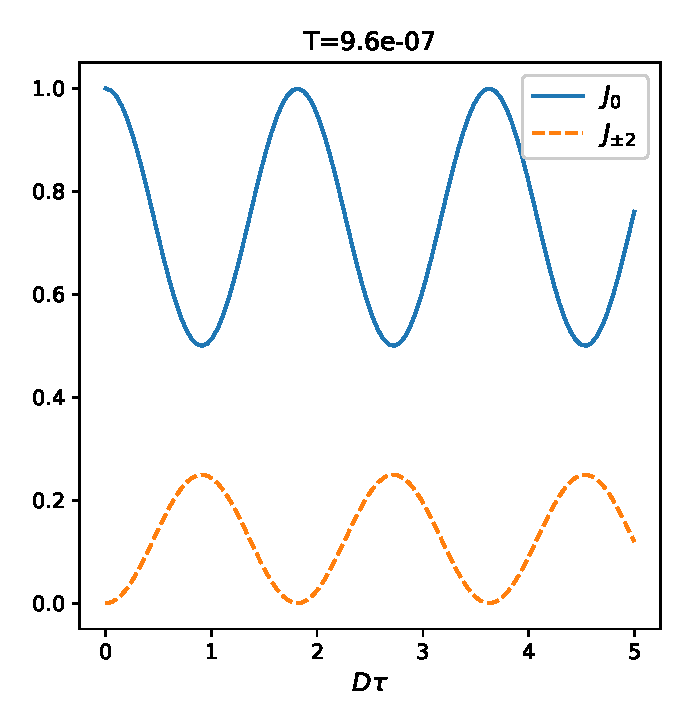
\includegraphics[width=0.5\linewidth]{coherences_n3_beta5.eps}
	\caption{
	  Интенсивности МК~когерентностей~ЯМР~$J_{n}$ ($n=0, 2$) в нанопоре с $N=3$.
      Здесь предполагается, что $\omega_{0} = 2\pi \cdot 500 \cdot 10^{6}$~s$^{-1}$ и $D = 2\pi \cdot 10^{4}$~s$^{-1}$.
	}
	\label{fig:1}
\end{figure}

В этом разделе будет получено точное решение МК~динамики~ЯМР~трехспиновой системы в дипольном упорядоченном состоянии в нанопоре.
Решение будет получена в общем виде, без использования высокотемпературного приближения~\cite{Goldman1970}.
Данная задача аналогична задаче, рассмотренной в разделе~\ref{sec:nanopora-thermodynamic-equilibrium}
для начального термодинамического равновесия в сильном внешнем магнитном поле.

Гамильтониан $H_{MQ}$ уравнения~(\ref{eq:hmq}) состоит из двух блоков для двух возможных значений углового момента спина $(I^2 = S(S+1), \quad S=3/2,1/2)$.
Эти блоки и соответствующие им собственные значения и собственные состояния приведены
в разделе~\ref{sec:sec:nanopora-thermodynamic-equilibrium-exact_sol}.
Матрица плотности системы также состоит из двух блоков $\rho^{3/2}(\tau)$, $\rho^{1/2}(\tau)$, и
%
\begin{equation}
  \label{eq:15}
  \rho^{3/2}(0) = \dfrac 1 Z
  \begin{pmatrix}
    e^{\frac{3b}{2}} & 0 & 0 & 0
    \\
    0 & e^{\frac{-3b}{2}} & 0 & 0
    \\
    0 & 0 & e^{\frac{-3b}{2}} & 0
    \\
    0 & 0 & 0 & e^{\frac{3b}{2}}
  \end{pmatrix},
  \quad
  \rho^{1/2}(0) = \dfrac 1 Z
  \begin{pmatrix}
    	1 & 0
    \\
    0 & 1
  \end{pmatrix}
\end{equation}
%
где $b = \dfrac{\hslash D}{k\mathrm{T}}$ и $T$ --- температура.
Простыми вычислениями можно получить матрицы плотности $\rho^{3/2}(\tau)$ и $\rho^{1/2}(\tau)$,
которые позволяют получить выражение для интенсивности МК~когерентностей~ЯМР.

В рассматриваемых системах появляются только МК~когерентности~ЯМР нулевого и плюс/минус второго порядков.
Интенсивности этих когерентностей равны
%
\begin{equation}
  \begin{split}
    \label{eq:16}
    J_0(\tau) & = 1
    - \dfrac 1 2 \tanh^2\left( \dfrac{3b}{2} \right)
      \sin^2 \left( \sqrt{3} Dt \right),
    \\
    J_{\pm2}(\tau) & = \dfrac{1}{4}
      \tanh^2 \left( \dfrac{3b}{2} \right)
      \sin^2 \left( \sqrt{3} Dt \right)
  \end{split}
\end{equation}
%
Сумма интенсивностей МК когерентностей согласно~(\ref{eq:16}) равна единице в соответствии с уравнением~(\ref{eq:14}).
Зависимости рассчитанных интенсивностей $J_{n}(\tau)$ $(n=0,2)$ от времени эволюции показаны на рисунке~(\ref{fig:1}).

% \subsection{Численный анализ многоспиновой запутанности при различных температурах и различном числе спинов в системе}
\subsection{Температурная зависимость многочастичной запутанности}
\label{sec:5}

В этом разделе приведены результаты полуаналитической симуляции МК эксперимента ЯМР
для модели спин-несущих молекул (атомов) в нанопоре в дипольном упорядоченном состоянии.
Будет рассмотрена зависимость нижней границы квантовой информации Фишера от времени и температуры.
А также получены оценки количества запутанных частиц в системе.
В расчетах предполагается, что $\omega_{0} = 2\pi \cdot 500 \cdot 10^{6}$~s$^{-1}$ и $D = 2\pi \cdot 10^{4}$~s$^{-1}$.

\begin{figure}[H]
 	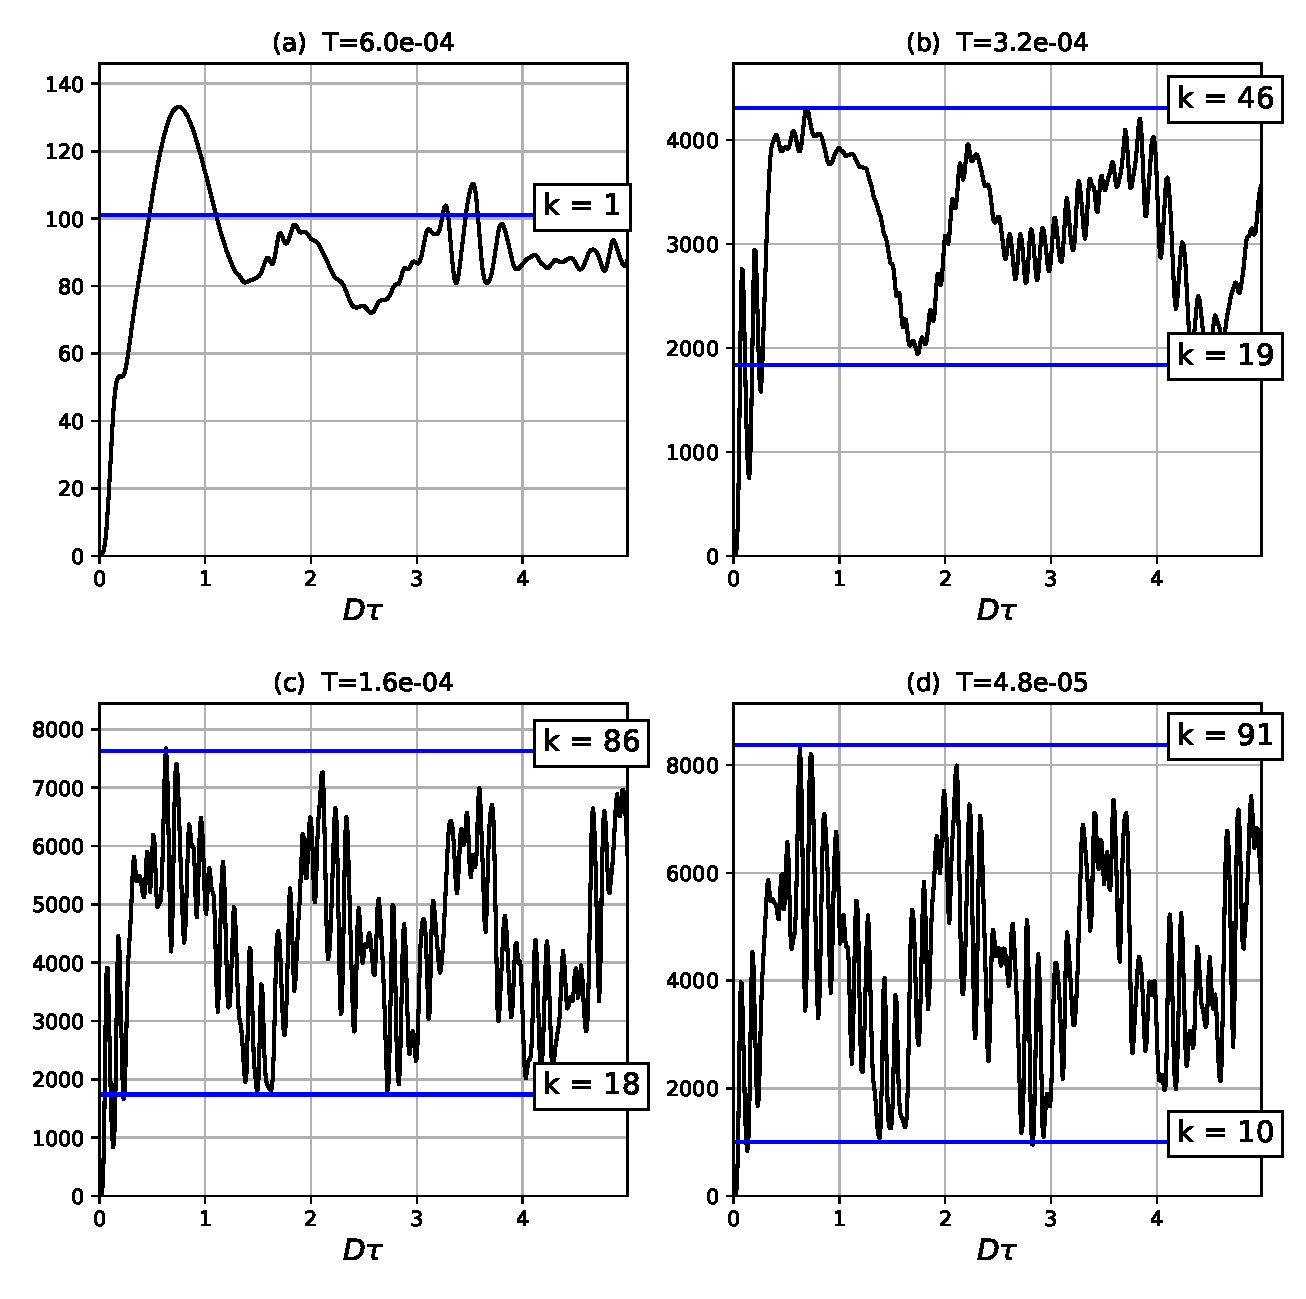
\includegraphics[width=0.95\linewidth]{fisher_low_bound_n101.eps}
	\caption{
	  Зависимость нижней границы  квантовой информации Фишера $F_\mathrm{Q} = 2 M_{2}$
	  от безразмерного времени $D\tau$ при $N=101$.
	  a) $T=6\cdot10^{-4}$~K, неравенство~(\ref{eq:20}) определяет область парной запутанности  (k+1=2), эта область выше горизонтальной линии;
	  b) $T=3.2\cdot10^{-4}$~K, область многоспиновой запутанности представляет собой полосу, ограниченную горизонтальными линиями с~$k=19$~и~$k=46$;
	  c) $T = 1.6\cdot10^{_4}$~K, горизонтальные линии ($k=18$ и $k=86$) ограничивают полосу с многоспиновой запутанностью;
	  d) при $T=4.8\cdot10^{-5}$~K возникают запутанные кластеры с $11-92$ спинами.
	}
	\label{fig:2}
\end{figure}


Рассматриваемая модель спин-несущих молекул (атомов) в нанопоре в дипольном упорядоченном состоянии
расширяет возможности исследования многоспиновой запутанности по сравнению с родственной моделью~(см. раздел~\ref{sec:nanopora-thermodynamic-equilibrium}),
в которой система изначально находилась в термодинамическом равновесии в сильном внешнем магнитном поле.
Модель из раздела~\ref{sec:nanopora-thermodynamic-equilibrium}) неприменима для исследования эволюции системы во времени,
потому что распределение МК~когерентностей~ЯМР~быстро становится стационарным~\cite{Doronin2009}.
Также многоспиновая запутанность изменяется с температурой в очень узком температурном интервале.
Например, все спины запутаны в системе, состоящей из 201 спина уже при температуре $T=6.856\cdot10^{-3}$~K~\cite{Doronin2019}.

Зависимость нижней границы квантовой информации Фишера от времени в системе, состоящей из 101 спина, представлена на Рис.~(\ref{fig:2}) при различных температурах.
Из Рис.~(\ref{fig:2}a) видно, что при температуре $T=6\cdot10^{-4}$~K существует только парная запутанность.
При температуре $T=3.2\cdot10^{-4}$ на Рис.~(\ref{fig:2}b) появляется полоса, в которой неравенство~(\ref{eq:entanglement-criteria}) может быть выполнено, когда $19 \leq k \leq 46$.
Таким образом, существует многоспиновая запутанность в спиновых кластерах, состоящих из 20-47 спинов, при температуре $3.2\cdot10^{-4}$~K.
Когда температура понижается, ширина полосы, в которой существует многоспиновая запутанность, увеличивается.
При температуре $T=1.6\cdot10^{-4}$~K (Рис.~(\ref{fig:2}c)) появляются кластеры из 19-87 запутанных спинов, а при температуре $T=4.8\cdot10^{-5}$~K (Рис.~(\ref{fig:2}d)), наблюдаются 11-92 запутанных спина.

\begin{figure}
 	\includegraphics[width=0.95\linewidth]{entangled_spins_by_n.eps}
	\caption{
	  Зависимость максимального количества запутанных спинов,
	  усредненного по времени эволюции $(0 \leq D\tau \leq 3)$,
	  от температуры при  a) $N=51$; b) $N=75$; c) $N=101$.
	}
	\label{fig:3}
\end{figure}

Зависимость максимального числа запутанных спинов за время эволюции $({0}\leq \mathrm{D}\tau\leq{3})$ от температуры при разных числах спинов в нанопоре представлена на Рис.~(\ref{fig:3}).
Максимальное количество запутанных спинов уменьшается при повышении температуры.
Максимальное количество запутанных спинов увеличивается, когда увеличивается число спинов в нанопоре, потому что система в нанопоре становится плотнее.

\section{Выводы}
\label{sec:conslusions}
% We investigated many-particle entanglement in MQ NMR spectroscopy using a nanocavity filled with spin-carrying atoms (molecules).
% We developed a theory of MQ NMR in a nanocavity at low temperatures.
% The theory is based on the idea that  molecular diffusion is substantially faster than the time of the spin flip-flop processes.
% As a result, the problem is reduced to a system of equivalent spins [23, 25], which can be analyzed in the basis of the common eigenstates of the total spin angular momentum and its projection on the external magnetic field.
% Since there is a connection between the second moment (dispersion) of the distribution of the MQ NMR intensities and many-spin entanglement [17], we extracted information about many-spin entanglement from the MQ NMR spectrum. The temperature dependence of many-spin entanglement was also investigated.
% \par
% The main lesson consists in significant growth of many-particle entanglement at low temperatures.
% All or almost all spins are entangled at the dimensionless temperature $\frac{1}{b}$ of the order of 1.
% This suggests that $k$-entangled states with large $k$ emerge in a typical MQ NMR system at low temperatures.
% This is particularly interesting given the absence of entanglement in the initial state. We expect such behavior to be typical for MQ NMR.
% \par
% We can conclude that MQ NMR spectroscopy is an effective method for the investigation of many-spin entanglement and the spreading of MQ correlations inside many-spin systems. It can be used for experimental investigations of quantum information processing in solids (note a related study of decoherence in liquids \cite{HOU2017863}).
% \par

В этой главе была исследована многочастичная запутанность в МК спектроскопии ЯМР в нанопоре, заполненной сотнями спин-несущими частицами.
Для этого была разработана МК теория ЯМР в нанопоре при низких температурах.
Было рассмотрено два начальных состояния системы:
термодинамически равновесное
и дипольное упорядоченное.
В обоих случах впервые удалось исследовать температурную зависимость многочастичной запутанности.
Все или почти все спины запутаны при безразмерной температуре $\frac{1}{b}$ порядка 1.
Это говорит о том, что $k$-запутанные состояния с большим $k$ возникают в типичной системе МК ЯМР при низких температурах.
Это особенно интересно, учитывая отсутствие запутанности в начальном состоянии.
Можно заключить, что такое поведение типично для МК ЯМР.
Так же была исследована зависимость многоспиновой запутанности
от количества спинов в нанопоре.
Показано, что с ростом количества спинов в нанопоре,
скорость возникновения запутанных кластеров при понижении температуры увеличивается.

Результаты этого раздела наглядно демонстрируют
универсальность разработанного в этой диссертации метода исследования многочастичной запутанности.

\begin{frame}{Эволюция нижней границы информации Фишера}
% (AMR-20)\footnote{G.A. Bochkin et al., \textit{Appl. Magn. Res.} \textbf{51}, 667-678, (2020)}
\begin{columns}

    \column{0.6\textwidth}
    \begin{figure}
    
\includegraphics[width=0.95\textwidth]{result-zchain-m2-by-time-n6-beta10.eps}
    %\caption{Hанопора со спин-несущих молекулами во внешнем сильном магнитном поле $\vec B$}
    \end{figure}

    \column{0.4\textwidth}
    Зависимость нижней границы квантовой информации Фишера
    $$ F_Q = 2M_2(\tau, T) $$
    от безразмерного времени $D_1 \tau$
    для шести спинов
    при температуре $T = 2.5 \times 10^{-3}$ $(\beta = 10)$.
    Область многочастичной запутанности ограничена горизонтальными линиями $k = 1$, $k = 5$.
\end{columns}
\end{frame}
\note{
   Мы не можем точно сказать сколько спинов запутанно,
   но можем дать нижнюю оценку на количество запутанных между собой спинов.
}


\begin{frame}{Максимальное количество запутанных спинов}
\begin{columns}

    \column{0.5\textwidth}
    \begin{figure}
    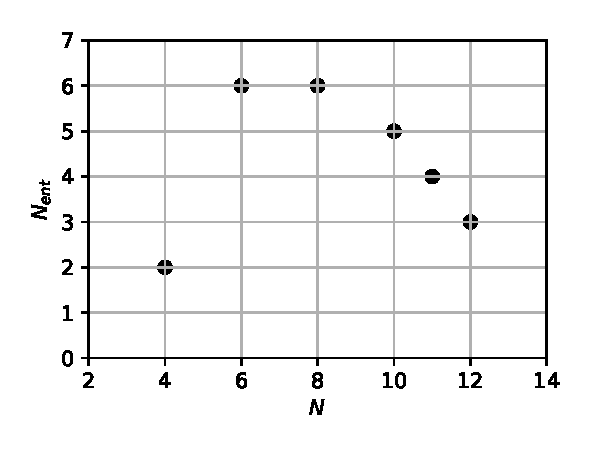
\includegraphics[width=\textwidth]{result-zchain-nent-by-n-beta10.eps}
    \caption{}
    \end{figure}

    \column{0.5\textwidth}
    Зависимость максимального количества запутанных спинов $N_\mathrm{ent}$ от длины цепи при температуре $T = 2.5 \times 10^{-3}$ $(\beta = 10)$.

    \vspace{0.5cm}

    \alert{Создание запутанных кластеров в рассматриваемых зигзагообразных цепочках ограничено слабыми дипольными взаимодействиями удаленных спинов}.
\end{columns}
\end{frame}
\note{
  Установлено что, при фиксированной температуре с ростом числа спинов в цепи размер запутанных кластеров может уменьшаться;
}


\begin{frame}{Максимальное количество запутанных спинов}
  \begin{columns}
     \column{0.5\textwidth}
     \begin{figure}
     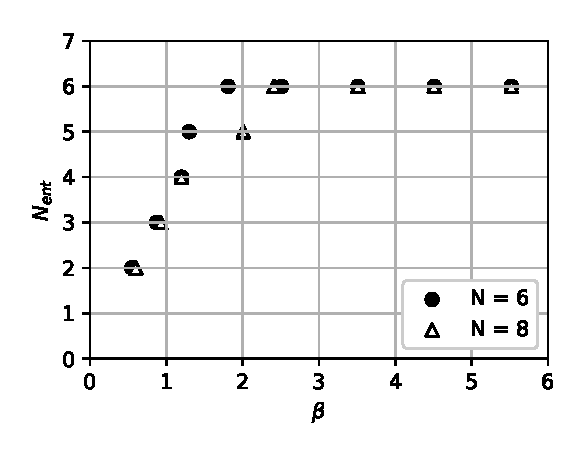
\includegraphics[width=\textwidth]{result-zchain-nent-by-beta-n8-n6.eps}
     \caption{}
     \end{figure}

     \column{0.45\textwidth}
     \begin{block}{}
       Зависимость максимального количества запутанных спинов $N_\mathrm{ent}$ от обратной температуры
       $$ \beta = \dfrac{\hbar\omega_0}{kT} $$
       в зигзагообразной цепочки из 6 и 8 спинов.
    \end{block}
  \end{columns}
\end{frame}
\note{
    Для 6 спинов накачка происходит быстрее, чем для 8 спинов.
}

\chapter{Измерение информации Вигнера-Янасе в МК эксперименте ЯМР}
\label{chapter:wyi-mesuarement}

% PLA-2021
\item
Разработана теория МК ЯМР в системе эквивалентных спинов s=1/2 при произвольных температурах. При низких температурах эта теория применена для расчетов многоспиновой запутанности в
нанопоре и зигзагообразной цепочке. 
Проведенные исследования позволяют заключить, что МК-спектроскопия ЯМР является тонким и полезным методом для исследования различных проблем квантовой информатики.

\item
Исследована температурная зависимость многочастичной запутанности в нанопоре с термодинамическим равновесным зеемановским и дипольно упорядоченным начальными состояниями. 
С понижением температуры количество запутанных спинов растет.
При температуре
$T = 6.856\cdot10^{-3}$~K $(\beta=3.5)$
почти все спины (до 179 из 201) запутаны. 
Можно заключить, что в типичной системе МК ЯМР при низких температурах возникают многочастичные запутанные состояния,
даже при отсутствии запутанности в начальном состоянии.  


\item
Исследована многочастичная запутанность в квазиодномерных цепочках ядерных спинов в зависимости от параметров цепи и температуры.
В однородных цепочках детектируется только парная запутанность, что согласуется с результатами, представленными в литературе.
В зигзагообразной цепочке при низких температурах почти все спины запутанны, так же как и в нанопоре.

\item
Предложен метод экспериментального измерения точного значения косой информации Вигнера-Янасе в рамках МК спектроскопии ЯМР.
Разработанный метод позволяет не только исследовать многочастичную запутанность методами МК ЯМР,
но и открывает возможность решения широкого класса задач квантовой теории информации.


\begin{thebibliography}{}

\bibitem{Einstein1935} A. Einstein, B. Podolsky, and N. Rosen \textit{Phys. Rev.} \textbf{47}, 777 (1935)
\bibitem{Bell1964} J.S. Bell \textit{Physics Physique Fizika} \textbf{1}, 195 (1964)
\bibitem{Scheidl2010} T. Scheidl et al. \textit{PNAS} \textbf{107}, 46, 19708-19713 (2010)

\bibitem{Bernabeu2012} Bernabéu, J., Martínez-Vidal, F. and Villanueva-Pérez, P. J. High Energ. Phys. 2012, 64 (2012).

\bibitem{Alain1976} Alain Aspect Phys. Rev. D 14, 1944 – Published 15 October 1976

% Zeqian Chen Phys. Rev. A 71, 052302
\bibitem{Gisin1991} N. Gisin, Phys. Lett. A 154, 201 (1991).
\bibitem{Clauser1969} J. F. Clauser, M. A. Horne, A. Shimony, and R. A. Holt, Phys. Rev. Lett. 23, 880 (1969).
\bibitem{Seevinck2002} M. Seevinck and G. Svetlichny, ibid. 89, 060401 (2002).
\bibitem{Uffink2002}  J. Uffink, Phys. Rev. Lett. 88, 230406 (2002O); K. Nagata, M. Koashi, and N. Imoto, ibid. 89, 260401 (2002).
%

\bibitem{Bennett1996} C.H.Bennett et al. \textit{Phys. Rev. A} \textbf{54}, 3824 (1996)
\bibitem{Eisert2001} Eisert J. and Briegel H. J. \textit{Phys. Rev. A} \textbf{64}, 022306 (2001)
\bibitem{Wootters1998} W.K. Wootters, \textit{Phys. Rev. Lett.} \textbf{80}, 2245 (1998)


% [5 - 31] P. Hyllus et al. Phys. Rev. A 85, 022321 (2012)
\bibitem{Plenio2007} M.B. Plenio and S. Virmani, Quant. Inf. Comp. 7, 1 (2007).
\bibitem{Amico2008} L. Amico, R. Fazio, A. Osterloh, and V. Vedral, Rev. Mod. Phys. 80, 517 (2008).
\bibitem{Horodecki2009} R. Horodecki, P. Horodecki, M. Horodecki, and K. Horodecki, Rev. Mod. Phys. 81, 865 (2009).
\bibitem{Guhne2009} O. G\"uhne and G. Toth, Physics Reports 474, 1 (2009).
\bibitem{Bourennane2004} M. Bourennane, M. Eibl, C. Kurtsiefer, S. Gaertner, H. Weinfurter, O. G\"uhne, P. Hyllus, D. Bruß, M. Lewenstein, and A. Sanpera, Phys. Rev. Lett. 92, 087902
\bibitem{Kaszlikowski2008} D. Kaszlikowski and A. Kay, New. J. Phys. 10, 053026 (2008).
\bibitem{Krammer2009} P. Krammer, H. Kampermann, D. Bruß, R.A. Bertlmann, L.C. Kwek, C. Macchiavello, Phys. Rev. Lett. 103, 100502 (2009).
\bibitem{Bancal2011} J.-D. Bancal, N. Gisin, Y.-C. Liang, and S. Pironio, PRL 106, 250404 (2011).
\bibitem{Svetlichny1987} G. Svetlichny, Phys. Rev. D 35, 3066 (1987).
\bibitem{Gisin1998} N. Gisin and H. Bechmann-Pasquinucci, Phys. Lett. A 246, 1 (1998).
\bibitem{Collins2002} D. Collins, N. Gisin, S. Popescu, D. Roberts, and V. Scarani, Phys. Rev. Lett. 88, 170405 (2002).
\bibitem{Seevinck2001} M. Seevinck and J. Uffink, Phys. Rev. A 65, 012107 (2001);
\bibitem{Toth2005} G. T\'oth, O. G\"uhne, M. Seevinck, and J. Uffink, Phys. Rev. A 72, 014101 (2005).
\bibitem{Nagata2002} K. Nagata, M. Koashi, and N. Imoto, Phys. Rev. Lett. 89, 260401 (2002).
\bibitem{Yu2003} S. Yu, Z.-B. Chen, J.-W. Pan, and Y.-D. Zhang, Phys. Rev. Lett. 90, 080401 (2003)
\bibitem{Laskowski2005} W.Laskowski and M.Zukowski, Phys.Rev.A72, 062112 (2005).
\bibitem{Schmid2008} C. Schmid, N. Kiesel, W. Laskowski, W. Wieczorek, and M.Z\'ukowski,and H.Weinfurter,Phys.Rev.Lett.100, 200407 (2008).
\bibitem{Bancal2009} J.-D. Bancal, C. Branciard, N. Gisin, and S. Pironio, Phys. Rev. Lett. 103, 090503 (2009).
\bibitem{Sorensen2001} A.S. Sørensen and K. Mølmer, Phys. Rev. Lett. 86, 4431 (2001).
\bibitem{Durkin2005} G.A. Durkin and C. Simon, Phys. Rev. Lett. 95, 180402 (2005).
\bibitem{Vitagliano2011} G. Vitagliano, P. Hyllus, I.L. Egusquiza, G. T\'oth, Phys. Rev. Lett. 107, 240502 (2011).
\bibitem{Duan2011} L.-M. Duan, Phys. Rev. Lett. 107, 180502 (2011).
\bibitem{Guhne2010} O. Guhne and M. Seevinck, New J. Phys. 12, 053002 (2010).
\bibitem{Huber2010} M. Huber, F. Mintert, A. Gabriel, and B.C. Hiesmayr, Phys. Rev. Lett. 104, 210501 (2010).
\bibitem{Li2010} C.-M. Li, K. Chen, A. Reingruber, Y.N. Chen, and J.W. Pan, Phys. Rev. Lett. 105, 210504 (2010).
\bibitem{Jungnitsch2011} B. Jungnitsch, T. Moroder, and O. G\"uhne, Phys. Rev. Lett. 106, 190502 (2011).
\bibitem{Vicente2011} J.I. de Vicente and M. Huber, Phys. Rev. A 84, 062306 (2011).
\bibitem{Huber2011} M. Huber, P. Erker, H. Schimpf, A. Gabriel, and B. Hiesmayr, Phys. Rev. A 83, 040301(R) (2011).
%---


\bibitem{Zeqian2005} Zeqian Chen \textit{Phys. Rev. A} \textbf{71}, 052302 (2005)

\bibitem{Hyllus2012} P. Hyllus et al. \textit{Phys. Rev. A} \textbf{85}, 022321 (2012)


% [19] Phys. Rev. A 71, 052302 (2005)
\bibitem{Wheeler2004} J.Wheeler, in Complexity, Entropy, and Physics of Information, edited by Z.H.Zurek (Addison-Wesley, Reading, MA, 1990), pp.3-28;
\bibitem{Summhammer2004}
J.Summhammer, Int.J.Theor.Phys. 33, 171(1994);
\bibitem{Frieden2004} B.R.Frieden, Science from Fisher Information: A Unification(Cambridge University Press, Cambridge, England, 2004).

\bibitem{khitrin1997} A. Khitrin, Chem. Phys. Lett. 274, 217 (1997)

\bibitem{g_arttner2018} M. G\"arttner, P. Hauke, and A. M. Rey, Phys. Rev. Lett. 120, 040402 (2018)

\bibitem{t_oth2014} G. T\"oth and I. Apellaniz, J. Phys. A 47, 424006 (2014)

\bibitem{pezz_e2018} L. Pezz\'e, A. Smerzi, M. K. Oberthaler et al., Rev. Mod. Phys. 90, 035005 (2018).

\bibitem{liu2014} J. Liu, H.-N. Xiong, F. Song, and X. Wang, Physica A 410, 167 (20


% Quatntum Fisher Information
\bibitem{Helstrom1976} C. W. Helstrom, Quantum detection and estimation theory, Academic Press, New York, 1976.
\bibitem{Holevo1982} A. S. Holevo, Probabilistic and statistical aspects of quantum theory, North-Holland, Amsterdam, 1982.


% Wigner yanase

% 10.1103/PhysRevLett.91.180403
% [3]
\bibitem{Araki1961} H. Araki and M. M. Yanase, Phys. Rev. 120, 622 (1960). [4] M. M. Yanase, Phys. Rev. 123, 666 (1961).
% [5]
\bibitem{Ozawa1991} M. Ozawa, Phys. Rev. Lett. 67, 1956 (1991).
% [6]
\bibitem{Ozawa2002a} M. Ozawa, Phys. Rev. Lett. 88, 050402 (2002).
% [7]
\bibitem{Ozawa2002b} M. Ozawa, Phys. Rev. Lett. 89, 057902 (2002).
% [8]
\bibitem{Matsumoto1993} S. Matsumoto, Prog. Theor. Phys. 90, 35 (1993).
% [9]
\bibitem{Kakazu3469} K. Kakazu and S. Pascazio, Phys. Rev. A 51, 3469
(1995).

% Chen2005
% 10.1103/PhysRevA.71.052302
% 3
% \bibitem{Einstein1935} A. Einstein, B. Podolsky, and N. Rosen, Phys. Rev. 47, 777 (1935).
% % 4
% \bibitem{Gisin1991} N. Gisin, Phys. Lett. A 154, 201 (1991).
% % 5
% \bibitem{Clauser1969} J. F. Clauser, M. A. Horne, A. Shimony, and R. A. Holt, Phys. Rev. Lett. 23, 880 (1969).
% ��6�� D. Collins, N. Gisin, S. Popescu, D. Roberts, and V. Scarani,
% Phys. Rev. Lett. 88, 170405 ��2002��; M. Seevinck and G.
% Svetlichny, ibid. 89, 060401 ��2002��.
% ��7�� J. Uffink, Phys. Rev. Lett. 88, 230406 ��2002��; K. Nagata, M.
% Koashi, and N. Imoto, ibid. 89, 260401 ��2002��.
% ��8�� S.-X. Yu, Z.-B. Chen, J.-W. Pan, and Y.-D. Zhang, Phys. Rev.
% Lett. 90, 080401 ��2003��.
% ��9�� E. P. Wigner, Z. Phys. 133, 101 ��1952��; Physikertagung Wien
% ��Physik-Verlag, Mosbach, 1952��, p. 1.

% E. P. Wigner and M. M. Yanase, \textit{Proc. Nat. Acad. Sci. USA}, \textbf{49}, 910–918 (1963)
% [1]
\bibitem{Weaver1949} W. Weaver's article in The Mathematical Theory of Communication (Urbana: The University of IllinoisPress,1949),p.45. SeealsothelastfewpagesofM.v.Smoluchowski'sarticleinVortrage fiberdie kinetische Theorie der Materie und Elektrizit4t (Leipzig: B. G. Teubner, 1914).
% [2]
\bibitem{Wigner1960} Wigner, E. P., Z. Physik, 131, 101 (1952); Araki, H., and M. M. Yanase, Phys. Rev., 120, 622(1960).
% [3]
\bibitem{Wigner1962} Wigner,E.P.,PhysikertagungWien(Mosbach/Baden: PhysikVerlag,1962),p.1

\bibitem{Wigner1963} E. P. Wigner and M. M. Yanase, \textit{Proc. Nat. Acad. Sci. USA}, \textbf{49}, 910–918 (1963) https://www.pnas.org/doi/abs/10.1073/pnas.49.6.910

\bibitem{Luo2003} S. Luo, \textit{Phys. Rev. Lett.} \textbf{91}, 180403 (2003)

\bibitem{Lieb1973prl} E. H. Lieb and M. B. Ruskai, “A fundamental property of quantum-mechanical entropy,” Phys. Rev. Lett., 30, 434–436 (1973).
\bibitem{Lieb1973} E. H. Lieb, “Convex trace functions and the Wigner–Yanase–Dyson conjecture,” Adv. Math., 11, 267–288 (1973).
\bibitem{Wehrl1978} A. Wehrl, “General properties of entropy,” Rev. Modern Phys., 50, 221–260 (1978).

\bibitem{Luo2005} S. L. Luo, “Quantum versus classical uncertainty,” Theor. Math. Phys., 143, 681–688 (2005).
\bibitem{Luo2005pra} S. Luo, “Heisenberg uncertainty relation for mixed states,” Phys. Rev. A, 72, 042110 (2005).
\bibitem{Luo2006} S. Luo, “Quantum uncertainty of mixed states based on skew information,” Phys. Rev. A, 73, 022324 (2006).
\bibitem{Luo2017pra} S. Luo and Y. Sun, “Quantum coherence versus quantum uncertainty,” Phys. Rev. A, 96, 022130 (2017).

\bibitem{Luo2020} S. Luo, Theoretical and Mathematical Physics, 202(1): 104–111 (2020)
% [9-23] Luo, Theoretical and Mathematical Physics, 202(1): 104–111 (2020)
% 9.
\bibitem{Luo2012} S. Luo, S. Fu, and C. H. Oh, “Quantifying correlations via the Wigner–Yanase skew information,” Phys. Rev. A,
85, 032117 (2012).
%10.
\bibitem{Li2016a} L. Li, Q.-W. Wang, S.-Q. Shen, and M. Li, “Measurement-induced nonlocality based on Wigner–Yanase skew
information,” Europhys. Lett., 114, 10007 (2016).
%11.
\bibitem{Sun2017} Y. Sun, Y. Mao, and S. Luo, “From quantum coherence to quantum correlations,” Europhys. Lett., 118, 60007
(2017).
% 12.
\bibitem{Girolami2014} D. Girolami, “Observable measure of quantum coherence in finite dimensional systems,” Phys. Rev. Lett., 113,
170401 (2014); arXiv:1403.2446v3 [quant-ph] (2014).
% 13.
\bibitem{Yu2017} C. Yu, “Quantum coherence via skew information and its polygamy,” Phys. Rev. A, 95, 042337 (2017); arXiv:
1704.04871v1 [quant-ph] (2017).
% 14.
\bibitem{Luo2017} S. Luo and Y. Sun, “Partial coherence with application to the monotonicity problem of coherence involving skew
information,” Phys. Rev. A, 96, 022136 (2017).
% 15.
\bibitem{Luo2018} S. Luo and Y. Sun, “Coherence and complementarity in state-channel interaction,” Phys. Rev. A, 98, 012113
(2018).
% 16.
\bibitem{Karpat2014} G. Karpat, B. Cakmak, and F. F. Fanchini, “Quantum coherence and uncertainty in the anisotropic XY chain,”
Phys. Rev. B, 90, 104431 (2014); arXiv:1404.6427v3 [quant-ph] (2014).
% 17.
\bibitem{Malvezzi2016} A. L. Malvezzi, G. Karpat, B. Cakmak, F. F. Fanchini, T. Debarba, and R. O. Vianna, “Quantum correlations
and coherence in spin-1 Heisenberg chains,” Phys. Rev. B, 93, 184428 (2016); arXiv:1602.03731v2 [quant-ph]
(2016).
% 18.
\bibitem{Li2016b} Y.-C. Li and H.-Q. Lin, “Quantum coherence and quantum phase transitions,” Sci. Rep., 6, 26365 (2016).
% 19.
\bibitem{Lei2016} S. Lei and P. Tong, “Wigner–Yanase skew information and quantum phase transition in one-dimensional quantum spin-1/2 chains,” Quantum Inf. Process., 15, 1811–1825 (2016).
% 20.
\bibitem{Qiu2017} L. Qiu, D. Quan, F. Pan, and Z. Liu, “Skew information in the XY model with staggered Dzyaloshinskii–Moriya
interaction,” Phys. B, 514, 13–18 (2017).
% 21.
\bibitem{Yanagi2005} K. Yanagi, S. Furuichi, and K. Kuriyama, “A generalized skew information and uncertainty relation,” IEEE Trans. Inform. Theory, 51, 4401–4404 (2005).
% 22.
\bibitem{Furuichi2010} S. Furuichi, “Schrodinger uncertainty relation with Wigner–Yanase skew information,” Phys. Rev. A, 82, 034101 (2010); arXiv:1005.2655v2 [quant-ph] (2010).
% 23.
\bibitem{Chen2016} B. Chen, S.-M. Fei, and G.-L. Long, “Sum uncertainty relations based on Wigner–Yanase skew information,” Quantum Inf. Process., 15, 2639–2648 (2016); arXiv:1606.01533v1 [quant-ph] (2016).
/Furuichi2010


% mq expreimetn
\bibitem{Baum1985} J. Baum, M. Munowitz, A. N. Garroway, and A. Pines, J. Chem. Phys. 83, 2015 (1985).


% models
\bibitem{Baugh2001}J. Baugh, A. Kleinhammes, D. Han, Q. Wang, and Y. Wu, \textit{Science} \textbf{294}, 1505 (2001).


% MQ NMR

%% Master diploma
\bibitem{vesta} Koichi Momma and Fujio Izumi. VESTA 3 for three-dimensional visualization of crystal, volumetric and morphology data. Journal of Applied Crystallography, 44(6):1272–1276, Dec 2011.

\bibitem{Elliott1994} J. C. Elliott. Structure and chemistry of the apatites and other calcium orthophosphates. Studies in Inorganic Chemistry 18. Elsevier Science, Amsterdam, 1994.

%% JETP Lett. 2015
%\bibitem{Baum1985} J. Baum, M. Munoviz, A. N. Garroway, and A. Pines. Multiple quantum dynamics in solid state NMR. The Journal of Chemical Physics, 83(5):2015– 2025, 1985.

%%
\bibitem{Bochkin2019jmr} G.A. Bochkin, E.B. Fel’dman, I.D. Lazarev, A.A. Samoilenko, S.G. Vasil’ev, Orientational dependencies of dynamics and relaxation of multiple quantum NMR coherences in one-dimensional systems, Journal of Magnetic Resonance (2019), doi: https://doi.org/10.1016/j.jmr.2019.02.004

%% JMR 2020
% []
% [1]
% \bibitem{Baum1985} J. Baum, M. Munowitz, A.N. Garroway, A. Pines, J. Chem. Phys. 83 (5) (1985) 2015–2025.
% [2]
\bibitem{Hughes2004} C.E. Hughes, Prog. Nucl. Magn. Reson. Spectrosc. 45 (3–4) (2004) 301–313.
% [3]
\bibitem{Vasilev2018} S.G. Vasil’ev, V.I. Volkov, E.A. Tatarinova, A.M. Muzafarov, N.A. Sipyagina, S.A. Lermontov, J. Non-Cryst. Solids 489 (2018) 6–15.
% [4]
\bibitem{Avilova2019} I.A. Avilova, A.V. Chernyak, S.G. Vasil’ev, Appl. Magn. Resonan. 50 (12) (2019) 1419 –1428.
% [5]
\bibitem{Mogami2014} Y. Mogami, S. Yamazaki, S. Matsuno, K. Matsui, Y. Noda, K. Takegoshi, Cem. Concr. Res. 66 (2014) 115–120.
% [6]
\bibitem{Krojanski2006} H.G. Krojanski, D. Suter, Phys. Rev. A 74 (6) (2006) 062319.
% [7]
\bibitem{Cho2006} H. Cho, P. Cappellaro, D.G. Cory, C. Ramanathan, Phys. Rev. B 74 (22) (2006) 224434.
% [8]
\bibitem{Bochkin2018} G.A. Bochkin, E.B. Fel’dman, S.G. Vasil’ev, V.I. Volkov, Appl. Magn. Reson. 49 (1) (2018) 25–34.
% [9]
\bibitem{Sanchez2014} C.M. S\'anchez, R.H. Acosta, P.R. Levstein, H.M. Pastawski, A.K. Chattah, Phys. Rev. A 90 (4) (2014) 042122.
% [10]
\bibitem{Alvarez2015} G.A. \'Alvarez, D. Suter, R. Kaiser, Science 349 (6250) (2015) 846–848.
% [11]
\bibitem{Wei2018} K.X. Wei, C. Ramanathan, P. Cappellaro, Phys. Rev. Lett. 120 (7) (2018) 070501.
% [12]
\bibitem{Garttner2018} M. G\"arttner, P. Hauke, A.M. Rey, Phys. Rev. Lett. 120 (4) (2018) 040402.
% [13]
\bibitem{Doronin2019} S.I. Doronin, E.B. Fel’dman, I.D. Lazarev, Phys. Rev. A 100 (2) (2019) 022330.
% [14]
\bibitem{Starkov2020}  G.A. Starkov, B.V. Fine, Phys. Rev. B 101 (2) (2020) 024428.
% [15]
\bibitem{Zhang2009} W. Zhang, P. Cappellaro, N. Antler, B. Pepper, D.G. Cory, V.V. Dobrovitski, C. Ramanathan, L. Viola, Phys. Rev. A 80 (5) (2009) 052323.
% [16]
\bibitem{Feldman2014} E.B. Fel’dman, Appl. Magn. Reson. 45 (8) (2014) 797–806.
% [17]
\bibitem{Feldman1997} E.B. Fel’dman, S. Lacelle, J. Chem. Phys. 107 (18) (1997) 7067–7084.
% [18]
\bibitem{Hayashi1960} S. Hayashi, Nippon kagaku zassi 81 (4) (1960) 540–542.
% [19]
\bibitem{Van1964} W. Van der Lugt, W.J. Caspers, Physica 30 (8) (1964) 1658–1666.
% [20]
\bibitem{ChoCho} G. Cho, J.P. Yesinowski, J. Phys. Chem. 100 (39) (Cho) 15716–15725.
% [21]
\bibitem{Itoh2005} K.M. Itoh, Solid State Commun. 133 (11) (2005) 747–752.
% [22]
\bibitem{Zachariasen1931} W.H. Zachariasen, Zeitschrift für Kristallographie - Crystalline Materials 76 (1) (1931) 289–302.
% [23]
\bibitem{Zachariasen1963} W.H. Zachariasen, H.A. Plettinger, M. Marezio, Acta Crystallogr. A 16 (11) (1963) 1144–1146.
% [24]
\bibitem{Gatta2012} G.D. Gatta, J.M. Garry, B. Geoffrey, G. Alessandro, N. Fabrizio, Am. Mineral. 97 (11–12) (2012) 1891–1897.
% [25]
\bibitem{Burns1995} P.C. Burns, M. Novak, F.C. Hawthorne, Can. Mineralogist 33 (6) (1995) 1205– 1213.
% [26]
\bibitem{Bochkin2019} G.A. Bochkin, E.B. Fel’dman, I.D. Lazarev, A.A. Samoilenko, S.G. Vasil’ev, J. Magn. Reson. 301 (2019) 10–18.
% [27]
\bibitem{Abragam1961} A. Abragam, The principles of nuclear magnetism, Clarendon Press, Oxford, 1961.
% [28]
\bibitem{Carolan1971} J.L. Carolan, Chem. Phys. Lett. 12 (2) (1971) 389–391.
% [29]
\bibitem{Vleck1948} J.H. Van Vleck, Phys. Rev. 74 (9) (1948) 1168–1183.
% [30]
\bibitem{Engelsberg1973} M. Engelsberg, I.J. Lowe, J.L. Carolan, Phys. Rev. B 7 (3) (1973) 924–929.
%% --


\end{thebibliography}


\end{document}
\begin{frame}{Определение информации Фишера в МК ЯМР (PRA-19)\footnote{S.I. Doronin, E.B. Fel'dman,  I.D. Lazarev, \textit{Phys. Rev. A}, \textbf{100}, 022330 (2019)}}
  $$ G(\tau, \phi) =
     \mathrm{Tr}\left\{
         e^{iH_\mathrm{MQ}\tau} e^{i\phi I_z} e^{-iH_\mathrm{MQ}\tau}
         \rho_\mathrm{eq}
         e^{iH_\mathrm{MQ}\tau} e^{-i\phi I_z} e^{-iH_\mathrm{MQ}\tau}
         I_z \right\}
  $$
  \begin{alertblock}{}
      Дисперсия распределения интенсивности МК когерентностей ЯМР определяет нижнюю границу информации
      Фишера\footnote[frame]{
      M. G\"arttner, P. Hauke, and A.M. Rey. \textit{Phys. Rev. Lett.} \textbf{120}, 040402 (2018)}:
      $$
      F_Q \geq 2M_2
      $$
  \end{alertblock}
  Однако формула справедлива только в том случае,
  если сигнал $G(\tau, \varphi)$ является \textit{out-of-time-ordered correlator} (OTOC).
  Для низких температур это условие не выполняется.
  Возможно обойти это ограничение,
  если усреднить сигнал МК эксперимента ЯМР по начальному состоянию:
  $$ G_\mathrm{LT}(\tau, \phi)
     = \mathrm{Tr}\left\{
       e^{iH_\mathrm{MQ}\tau} e^{i\phi I_z} e^{-iH_\mathrm{MQ}\tau}
       \rho_\mathrm{eq}
       e^{iH_\mathrm{MQ}\tau} e^{-i\phi I_z} e^{-iH_\mathrm{MQ}\tau}
       {\color{red} \rho_\mathrm{eq}}
    \right\}
  $$
\end{frame}



\chapter{Многоспиновая запутанность в системе эквивалентных спинов}
\label{chapter:manyparticle-entanglement-in-nanopore}
% \subsection{Создание дипольно упорядоченных состояний}
% (PRA-2019)
%   - Температурная зависимость многочастичной запутанности
%   - Зависимость от числа частиц
%
% Многоспиновая запутанность c дипольно упорядоченном начальном

% JETP-2020


Результат полученный в предыдущей главе~\ref{chapter:quantum-fisher-information-measurement}
позволяет в рамках МК динамики ЯМР прояснить более глубокие связи между MK когерентностями ЯМР и запутанностью.
Эти связи соответствуют распространению МК корреляций внутри многочастичной системы в процессе эволюции.
В результате из второго момента спектра интенсивности МК когерентностей ЯМР
можно извлечь информацию о многочастичной запутанности и свидетелях запутанности.

Для исследования многочастичной запутанности необходимо работать с моделью,
которая содержит достаточно большое ($>50$) количество взаимодействующих спинов,
и может быть экспериментально исследована при низких температурах.
Только тогда можно будет исследовать многочастичную запутанность и ее зависимость от температуры.
В разделе~\ref{sec:model-equivalent-spins} была рассмотрена несферическая нанопора,
заполненная газом со спин-несущими атомами (например, ксеноном) или молекулами в сильном внешнем магнитном поле.
Эта модель полностью отвечает поставленным требованиям.
По существу нанопора является системой эквивалентных спинов,
и ее МК динамика ЯМР может быть исследована точно.

На подготовительном периоде МК эксперимента ЯМР гамильтониан системы эквивалентных спинов
определяется выражением (см~\ref{sec:model-equivalent-spins})
\begin{equation}\label{eq:mq-hamiltoninan-equivalent-spins}
  H_\mathrm{MQ} = - \dfrac{D}{4} \left[
    \left( I^{+} \right)^2 + \left( I^{-} \right)^2
  \right],
  \quad
  I^{\pm} = \sum\limits_{j=1}^{N} I^{\pm}_j,
\end{equation}
где $I^{\pm}_{j}$ --- повышающий или понижающий операторы спина $j$,
$N$ --- число спинов в нанопоре,
$D$ - константа диполь-дипольного взаимодействия (ДДВ),
усредненная по быстрой молекулярной диффузии спин-несущих атомов (молекул) в нанопоре.
Как уже было обсуждено в разделе~\ref{sec:model-equivalent-spins},
гамильтониан $H_\mathrm{MQ}$
коммутирует с квадратом полного спинового углового момента $\hat I^2$,
поэтому удобно перейти к базису,
состоящего из общих собственных состояний $\hat I^2$ и $I_z$.
В этом базисе гамильтониан $H_{MQ}$ состоит из блоков $H_{MQ}^S$, соответствующих различным значениям полного спинового углового момента $S$:
\begin{equation}
  \hat I^2 = S(S+1), S = N/2, N/2-1, N/2-2,
\end{equation}
где
$N/2 - [N/2]$, $[i]$ - целая часть $i$.

Далее в этой главе будут рассмотрены два наиболее интересных начальных состояний системы
и исследованы температурные зависимости многоспиновой запутанности для каждого случая.

\section{Термодинамически равновесное начальное состояние}
\label{sec:nanopora-thermodynamic-equilibrium}

Для исследования многочастичной запутанности в зависимости от температуры,
в этом разделе будет рассмотрена МК динамика ЯМР
системы эквивалентных спинов размера $N$
с начальным термодинамически равновесным состоянием $\rho_\mathrm{eq}$:
%
\begin{equation}\label{eq:rho_eq}
  \rho(0) = \rho_{\mathrm{eq}} = \dfrac{e^{\frac{\hbar\omega_{0}}{kT} I_z}}{Z},
\end{equation}
%
где $Z =\mathrm{Tr}\left\{e^{\frac{\hbar\omega_{0}}{kT} I_z}\right\}$ это статистическая сумма,
$\hbar$ и $k$ --- это постоянная Планка и постоянная Больцмана,
$\omega_0$ --- Ларморовская частота,
$T$ --- температура,
и $I_z$ это оператор проекции полного углового момента на ось $z$,
которая направлена вдоль сильного внешнего магнитного поля.
%
Существующий теоретический подход~\cite{Doronin2009, Doronin2011}
к МК динамике ЯМР системы эквивалентных спинов
применим только в высокотемпературной области.
Для исследования многочастичной запутанности,
необходимо разработать теорию МК динамики ЯМР системы эквивалентных спинов
для произвольных температур,
что будет сделано ниже.
% Так же будут приведены вычисления для системы из 51, 75, 101, 201 спинов,
% но, в принципе, аналогичные расчеты можно провести и для систем с несколькими тысячами спинов.

Поскольку и гамильтониан $H_{MQ}$, и матрица начальной плотности из уравнения~(\ref{eq:rho_eq}) имеют блочную структуру,
можно заключить,
что эволюционная матрица плотности $\rho_\mathrm{LT}(\tau)$:
%
\begin{equation}
  \label{eq:rho_eval_lt}
  \rho_\mathrm{LT} (\tau) = e^{-iH_\mathrm{MQ}\tau} \rho_\mathrm{eq} e^{iH_\mathrm{MQ}\tau},
\end{equation}
%
также состоит из блоков $\rho^S_\mathrm{LT}(\tau)$,
где $(S=\frac N 2, \frac N 2 - 1, \dots, \frac N 2 - \left[\frac N 2\right])$.
Введем обозначение $\rho^S_{\mathrm{LT}, n}(\tau)$ для
вклада в $\rho^S_\mathrm{LT}(\tau)$ от МК когерентности ЯМР порядка $n$.
Тогда вклад $J_{\mathrm{LT}, n, S}(\tau)$ в интенсивность приведенной МК когерентности ЯМР $n$-го порядка определяется как
%
\begin{equation}
    \label{eq:coherence_k_s}
    J_{\mathrm{LT}, n, S}(\tau) = \dfrac{\mathrm{Tr}\left\{
        \rho_{LT, n}^S(\tau)\rho_{LT, -n}^S(\tau)
    \right\}}
    {\mathrm{Tr}\left\{\rho^2_{eq}\right\}}.
\end{equation}
%
Таким образом задача вычисления когерентностей сводится к вычислению отдельных вкладов для каждого значения полного углового момента $S$.

Наблюдаемые интенсивности приведенных МК когерентностей ЯМР рассчитываются по формуле:
%
\begin{equation}\label{eq:coherence_k}
  J_{\mathrm{LT}, n}(\tau) = \sum\limits_S n_N(S) J_{\mathrm{LT}, n, S}(\tau),
  \quad
  (-N\leq n \leq N),
\end{equation}
%
где $n_N(S)$ --- это кратность интенсивности $J_{n, S}(\tau)$,
определенная в разделе~\ref{sec:model-equivalent-spins} в~(\ref{eq:coeff_n}).


\subsection{Аналитическое решение для трехспиновой системы}
\label{sec:sec:nanopora-thermodynamic-equilibrium-exact_sol}

% \begin{figure}[H]
%   \centering
%   \includegraphics{exact_j.pdf}
%   \caption{Intensities of MQ NMR coherences $J_n, \quad n=0, 2$ in a nanopore with $N = 3$.}
%   \label{fig:exact_j}
% \end{figure}

В этом разделе будет рассмотрена система из $N=3$ спинов
связанных $H_{MQ}$ гамильтонианом,
определенном в выражении (\ref{eq:mq-hamiltoninan-equivalent-spins}).
Возможными значениями полного углового момента спина $S$
являются $\frac 3 2$ и $\frac 1 2$.
Ненулевые элементы блока гамильтониана $H_{MQ}^{S}$ определены в выражении~(\ref{eq:i-square-elements}).
Матричное представление $H_{MQ}^{3/2}$ имеет вид
%
\begin{equation}
    \label{eq:ham_3_2}
    H_{MQ}^{3/2} =
    \begin{pmatrix}
        0 & 0 & -\frac{\sqrt{3} D}{2} & 0 \\
        0 & 0 & 0 & -\frac{\sqrt{3} D}{2} \\
        -\frac{\sqrt{3} D}{2} & 0 & 0 & 0 \\
        0 & -\frac{\sqrt{3} D}{2} & 0 & 0
    \end{pmatrix}.
\end{equation}
%
Собственные значения $\lambda_{3/2}^{(i)}(i=1, 2, 3, 4)$
блока гамильтониана $H_{MQ}^{3/2}$ следующие
%
\begin{equation}\label{eq:eigvals_3_2}
  \lambda_{3/2}^{(1)} = -\frac{\sqrt{3} D}{2}, \quad
  \lambda_{3/2}^{(2)} = -\frac{\sqrt{3} D}{2}, \quad
  \lambda_{3/2}^{(3)} = \frac{\sqrt{3} D}{2}, \quad
  \lambda_{3/2}^{(4)} = \frac{\sqrt{3} D}{2}.
\end{equation}
%
Соответствующий набор собственных векторов выглядит следующим образом:
%
\begin{align}\label{eq:eigvecs_3_2}
  u_{3/2}^{(1)} & =  \left(\frac{1}{\sqrt{2}}, 0, \frac{1}{\sqrt{2}}, 0\right) ,
  \notag \\
  u_{3/2}^{(2)} & =  \left(0, \frac{1}{\sqrt{2}}, 0, \frac{1}{\sqrt{2}}\right) ,
  \notag \\
  u_{3/2}^{(3)} & =  \left(-\frac{1}{\sqrt{2}}, 0, \frac{1}{\sqrt{2}}, 0\right) ,
  \notag \\
  u_{3/2}^{(4)} & =  \left(0, -\frac{1}{\sqrt{2}}, 0, \frac{1}{\sqrt{2}}\right) .
\end{align}
%
Блок $H^{1/2}_{MQ}$ является скаляром
%
\begin{equation}\label{eq:ham_1_2}
  H^{1/2}_{MQ} = 0.
\end{equation}
%
Блоки эволюционной матрицы плотности $\rho_\mathrm{LT}^{n/2}(\tau) \quad (n = 1, 3)$
могут быть вычислены по формуле
%
\begin{equation}\label{eq:liouvile_sol}
  \rho_\mathrm{LT}^{n/2}(\tau) =
  U_{n/2} e^{-i\Lambda^{n/2}\tau} U^{+}_{n/2}
  \rho^{n/2}_\mathrm{LT}(0)
  U_{n/2} e^{i\Lambda^{n/2}\tau} U^{+}_{n/2},
\end{equation}
%
где $\Lambda^{n/2}$ --- диагональная матрица собственных значений,
$U_{n/2}$ --- матрица собственных векторов блока $H_{MQ}^{n/2} \quad (n=1, 3)$,
а начальная матрица плотности $\rho_\mathrm{LT}^{n/2}(0)$ имеет вид:
%
\begin{equation}\label{eq:rho_LT_init}
  \rho_\mathrm{LT}^{3/2}(0) = \dfrac 1 Z
  \begin{pmatrix}
      e^{\frac{3b}{2}} & 0 & 0 & 0
      \\
      0 & e^{\frac{b}{2}} & 0 & 0
      \\
      0 & 0 & e^{-\frac{b}{2}} & 0
      \\
      0 & 0 & 0 & e^{-\frac{3b}{2}}
  \end{pmatrix},
  \quad
  \rho_\mathrm{LT}^{1/2}(0) = \dfrac 1 Z
  \begin{pmatrix}
      e^{\frac{b}{2}} & 0
      \\
      0 & e^{-\frac{b}{2}}
  \end{pmatrix}.
\end{equation}
После вычисления выражений
(\ref{eq:eigvals_3_2}),
(\ref{eq:eigvecs_3_2}),
(\ref{eq:liouvile_sol})
и (\ref{eq:rho_LT_init}) с $n = 3$,
получаем
%
\begin{equation}\label{eq:rho_LT_eval_3_2}
  \rho_\mathrm{LT}^{3/2}(\tau) = \frac{1}{Z} \\
  \begin{pmatrix}
      ue^{-\frac{b}{2}} + ve^{\frac{3b}{2}}
    &
      0
    &
      -ie^{\frac{b}{2}}w
    &
      0
    \\
      0
    &
      ue^{-\frac{3b}{2}} + ve^{\frac{b}{2}}
    &
      0
    &
      -ie^{-\frac{b}{2}}w
    \\
      ie^{\frac{b}{2}}w
    &
      0
    &
      ue^{\frac{3b}{2}} + ve^{-\frac{b}{2}}
    &
      0
    \\
      0
    &
      ie^{-\frac{b}{2}}w
    &
      0
    &
      ue^{\frac{b}{2}} + ve^{-\frac{3b}{2}}
  \end{pmatrix},
\end{equation}
где
\begin{equation}
    u = \sin^2\left(\frac{\sqrt{3}}{2}D\tau\right),
    \quad
    v = \cos^2\left(\frac{\sqrt{3}}{2}D\tau\right),
    \quad
    w = \sin(b)\sin\left(\sqrt{3}D\tau\right).
\end{equation}
%
Аналогичные вычисления для матрицы $\rho^{1/2}_\mathrm{LT} (\tau)$
с использованием выражений (\ref{eq:liouvile_sol}) и (\ref{eq:rho_LT_init})
дают
%
\begin{equation}
\label{eq:rho_LT_eval_1_2}
    \rho_\mathrm{LT}^{1/2}(\tau) = \frac 1 Z
    \begin{pmatrix}
            e^{\frac b 2}
        &
            0
        \\
            0
        &
            e^{-\frac b 2}
    \end{pmatrix}.
\end{equation}

В рассматриваемой системе появляются только МК когерентности ЯМР нулевого и плюс/минус второго порядков.
Эти интенсивности могут быть вычислены с помощью выражений
(\ref{eq:coherence_k_s}), (\ref{eq:rho_LT_eval_3_2}) и (\ref{eq:rho_LT_eval_1_2})
%
\begin{align}\label{eq:j_lt_3}
  J_{\mathrm{LT}, 0}(\tau) & = 1 - \frac 1 2 \tanh^2(b)\sin^2(\sqrt 3 D \tau), \notag \\
  J_{\mathrm{LT},\pm 2}(\tau) & = \frac 1 4 \tanh^2(b)\sin^2(\sqrt 3 D \tau)
\end{align}
%
Можно убедиться что сумма интенсивностей~(\ref{eq:j_lt_3}) равна 1
и не зависит от времени $\tau$, так же как и в~(\ref{eq:sum_of_coherence}).
Профили рассчитанных интенсивностей $J_n(\mathrm{LT}, \tau)$, $(n=0,2)$ показаны на рис.~\ref{fig:exact_j}.


\subsection{Температурная зависимость многочастичной запутанности}
%\subsection{The temperature dependence of the many-particle entanglement}
\label{sec:entanglement}
В этом разделе приведены результаты полуаналитической симуляции МК эксперимента ЯМР
для модели спин-несущих молекул (атомов) в нанопоре в термодинамически равновесном состоянии.
Будет рассмотрена зависимость нижней границы квантовой информации Фишера от времени и температуры.
А также будут получены оценки количества запутанных частиц в системе,
состоящей из 201 спина.
% В расчетах предполагается, что $\omega_{0} = 2\pi \cdot 500 \cdot 10^{6}$~s$^{-1}$ и $D = 2\pi \cdot 10^{4}$~s$^{-1}$.

\begin{figure}[H]
  \centering
  \begin{subfigure}[t]{0.4\textwidth}
    %\centering
    \includegraphics[width=\textwidth]{m2_t_b01.pdf}
    \caption{
      ${T=2.4\cdot10^{-1}}$~K $(b=0.1)$.
      Парная запутанности выше горизонтальной линии.
      %The inequality~(\ref{eq:fisher_criteria}) yields the region of pair entanglement $(k+1=2)$.
      %The region is above the horizontal line.
    }
    \label{fig:m2_t_b01}
  \end{subfigure}
  \hfill
  \begin{subfigure}[t]{0.4\textwidth}
    %\centering
    \includegraphics[width=\textwidth]{m2_t_b05.pdf}
    \caption{
      ${T=4.8\cdot10^{-2}}$~K $(b=0.5)$.
      Область многоспиновой запутанности представляет собой полосу, ограниченную горизонтальными линиями с $k=14$ и $k=27$.
      }
    \label{fig:m2_t_b05}
  \end{subfigure}
  \hfill
  \begin{subfigure}[t]{0.4\textwidth}
    \includegraphics[width=\textwidth]{m2_t_b1.pdf}
    \caption{
      ${T=2.4\cdot10^{-2}}$~K $(b=1)$.
    }
    \label{fig:m2_t_b1}
  \end{subfigure}
  \hfill
  \begin{subfigure}[t]{0.4\textwidth}
    %\centering
    \includegraphics[width=\textwidth]{m2_t_b3_5.pdf}
    \caption{
      ${T=6.856\cdot10^{-3}}$~K $(b=3.5)$.
      Почти все спины (до $179$ из $201$) могут быть частью запутанного кластера.
    }
  \label{fig:m2_t_b3.5}
  \end{subfigure}
  \caption{
    Зависимость нижней границы квантовой информации Фишера $F_Q = 2M_2(\tau)$ от безразмерного времени $D\tau$.
    Горизонтальные линии ограничивают полосу с многоспиновой запутанностью.
  }
\end{figure}

Интенсивности приведенных МК когерентностей  ЯМР определяются уравнениями ~(\ref{eq:j_lt},~\ref{eq:j_lt_norm}) как при высоких ($b < 1$), так и при низких ($b > 1$) температурах.
Нижняя граница квантовой информации Фишера может быть посчитана из выражений
~(\ref{eq:j_lt}),~(\ref{eq:j_lt_norm}),~(\ref{eq:fisher-low-bound})~и~(\ref{eq:m2-via-coherences}).

Значение параметра $b = 0.1$, соответствует температуре ${T= 2.4\cdot 10^{-1}}$~K при Ларморовской частоте $\omega_0 = 2\pi\cdot 500\cdot10^6$ с$^{-1}$ (рис.~\ref{fig:m2_t_b01}).
Неравенство~(\ref{eq:entanglement-criteria}) может быть выполнено только при $k=1$ (горизонтальная линия на рис.~\ref{fig:m2_t_b01}).
Это означает, что парная запутанность возможна в высокотемпературном случае \cite{Feldman2012}.

При температуре ${4.8\cdot10^{-2}}$~K $(b=0.5)$ видна полоса (рис.~\ref{fig:m2_t_b05}), в которой неравенство~(\ref{eq:entanglement-criteria}) может быть удовлетворено, когда $14 \leq k \leq 27$.

Таким образом, при температуре ${4.8\cdot10^{-2}}$~K в спиновых кластерах, состоящих из 15-28 спинов, существует многоспиновая запутанность. При понижении температуры ширина полосы, где существует многоспиновая запутанность, увеличивается. При температуре ${2.4\cdot10^{-2}}$~K $(b=1)$ (рис.~\ref{fig:m2_t_b1}) в такой полосе число запутанных спинов может составлять от 36 до 92.

Наконец, при температуре ${T= 6.856\cdot10^{-3}}$~K $(b=3.5)$ (рис.~\ref{fig:m2_t_b3.5}), почти все спины (до 179 из 201) запутаны. Запутанность существует в течение всего процесса эволюции, за исключением короткого начального периода времени.

На рис.\ref{fig:k_b} показано, что количество запутанных спинов увеличивается при понижении температуры.


Таким образом, предложенная модель нанополости, заполненной спин-несущими атомами (молекулами), позволяет исследовать многоспиновую запутанность и ее зависимость от температуры.

\begin{figure}[H]
  \centering
  \includegraphics{k_b.pdf}
  \caption{Зависимость числа запутанных спинов от параметра  $b = \frac{\hbar\omega_0}{kT} $.}
  \label{fig:k_b}
\end{figure}



\section{Дипольное упорядоченное состояние}
\label{sec:1}

В предыдущем разделе~\ref{sec:nanopora-thermodynamic-equilibrium} была исследована многоспиновая запутанность для несферической нанопоры~\cite{Doronin2019},
заполненной газом  спин-несущих молекул в сильном внешнем магнитном поле~\cite{Baugh2001,Doronin2009}.
Термодинамическое равновесное начальное состояние системы определялось односпиновым зеемановским взаимодействием с внешним магнитным полем~\cite{Doronin2007a}.
Однако  многоспиновую запутанность можно  исследовать,
когда та же самая система первоначально подготовлена в дипольном упорядоченном состоянии~\cite{Goldman1970}.
Главной мотивацией выбора такого начального состояния является результат полученный в работе~\cite{Doronin2011}.
В частности было показано, что в МК~эксперименте~ЯМР~с дипольным упорядоченным начальным состоянием МК~когерентности~ЯМР~возникают быстрее,
чем в МК~эксперименте~ЯМР~с начальным термодинамическим равновесным состоянием в сильном внешнем магнитном поле.
Данное обстоятельство является важным для исследования многоспиновой запутанности,
поскольку при этом используется второй момент распределения МК~когерентностей~ЯМР.

В общем случае в начальный момент система находится в термодинамическом равновесии с матрицей плотности
%
\begin{equation}\label{eq:4}
    \rho(0) = \rho_\mathrm{eq} = \dfrac{1}{Z}
    e^{
      \frac{\hslash \omega_{0}}{k} \alpha_\mathrm{z} I_\mathrm{z}
      + \frac{\hslash }{k} \beta_\mathrm{d} H_\mathrm{dz}
    },
\end{equation}
%
где
$Z = \mathrm{Tr} \left\{ e^{\frac{\hslash \omega_{0}}{k} \alpha_\mathrm{z} I_\mathrm{z} + \frac{\hslash }{k} \beta_\mathrm{d} H_\mathrm{dz}} \right\}$ - статистическая сумма,
$\hslash$ и $k$ - константы Планка и Больцмана,
$\omega_{0}$ - частота Лармора,
$I_\mathrm{z}$ -  оператор проекции полного углового спинового момента  на ось~$z$,
который направлен вдоль сильного внешнего магнитного поля,
$H_\mathrm{dz}$ - секулярная часть гамильтониана ДДВ в сильном внешнем магнитном поле
и $\alpha_\mathrm{z}$, $\beta_\mathrm{d}$ - обратные зеемановская и дипольная температуры.
%
Используя  метод адиабатического размагничивания во вращающейся системе координат (ВСК)~\cite{Goldman1970, Slichter1961},
либо двухимпульную последовательность Брокаерта-Джинира~(см. подраздел~\ref{seq:jeener-sequence})
можно получить систему в состоянии термодинамического равновесия с матрицей плотности
%
\begin{equation}\label{eq:5a}
  \rho_i = \frac{1}{Z_i} e^\frac{\hslash\beta_\mathrm{d} \hdz}{k},
  %approx \frac{1}{Z_i}(1 + \frac{\hslash\beta_\mathrm{d}}{k} H_\mathrm{dz}),
\end{equation}
%
где статистическая сумма
%
\begin{equation}\label{eq:6}
  Z_i = \mathrm{Tr} \left\{ e^\frac{\hslash\beta_\mathrm{d} \hdz}{k} \right\} \approx 2^{N}.
\end{equation}
%
Магнитное упорядочение~\cite{Abragam1982} выходит за рамки данного раздела,
поэтому будет рассмотрен промежуточный температурный случай,
когда зеемановская температура является низкой $({\frac{\hslash \omega_{0}}{k} \alpha_\mathrm{z}}\gg 1)$,
а дипольная - высокой $\left( \frac{\hslash{D}}{k}\beta_\mathrm{d} \ll 1\right)$.
Тогда выражение~(\ref{eq:5a}) матрицы плотности~$\rho_i$ может быть разложено в ряд по $b$:
%
\begin{equation}\label{eq:5}
  \rho_i \approx \frac{1}{Z_i}(1 + \frac{\hslash\beta_\mathrm{d}}{k} H_\mathrm{dz}),
\end{equation}
%
Гамильтониан $H_{dz}$ частично усредняется быстрой молекулярной диффузией в нанопоре,
и может быть записан~\cite{Feldman2004,Doronin2011} как
%
\begin{equation}
  \label{eq:7}
  H_\mathrm{dz} = \dfrac{D}{2} (3 I^{2}_{z} - I^{2}) , % ?
\end{equation}
%
где $I^{2}$ - квадрат углового спинового  момента.

После периодов подготовки, эволюции и смешивания в МК~эксперименте~ЯМР~(см. раздел~\ref{sec:mq-nrm-experiment})
сигнал усредненный по равновесной матрице плотности $\rho_i$
имеет вид~(см. раздел~\ref{sec:reduced-mq-coherences})
%
\begin{equation}\label{eq:signal-do}
  \begin{split}
    G_\mathrm{DO}(\tau,\phi)
    & = \mathrm{Tr}\left\{
      e^{i H_\mathrm{MQ} \tau} e^{i\phi I_\mathrm{z}} e^{-i H_\mathrm{MQ}\tau}
      \rho_i
      e^{i H_\mathrm{MQ} \tau} e^{-i \phi I_\mathrm{z}} e^{-i H_\mathrm{MQ} \tau}
      \rho_i
    \right\} \\
    & = \mathrm{Tr} \left\{
    e^{i \phi I_\mathrm{z}}
    \rho_\mathrm{DO}(\tau)
    e^{-i \phi I_\mathrm{z}}
    \rho_\mathrm{DO}(\tau)
    \right\},
  \end{split}
\end{equation}
%
где
%
\begin{equation}
  \label{eq:9}
  \rho_\mathrm{DO}(\tau)
  = e^{-i H_\mathrm{MQ} \tau }
  \rho_i
  e^{i H_\mathrm{MQ} \tau}
\end{equation}
%
является решением уравнения~(\ref{eq:3}) при начальном условии~(\ref{eq:5}).
Выражение~\ref{eq:signal-d} сигнала  $G_\mathrm{DO}G_\mathrm{HT}(\tau,\phi)$,
является неупорядоченные по времени коррелятором~(см. раздел~\ref{sec:reduced-mq-coherences}),
следовательно, второй момент коррелятора $G_\mathrm{DO}(\tau,\phi)$ определяет
нижнюю границу квантовой информации Фишера~(см. раздел~\ref{sec:reduced-mq-coherences}).
Нормированные интенсивности $J_{n}(\tau)$ $(n=0, \pm 2, \pm 4, \cdots)$ МК~когерентностей~ЯМР
имеют вид
%
\begin{equation}\label{eq:13}
  J_{n}(\tau) = \dfrac{\mathrm{Tr} \left\{
  \rho_{n}(\tau) \rho_{-n}(\tau)
  \right\}}
  {\mathrm{Tr} \left\{\rho^2_{i} \right\}}
\end{equation}


Матрица плотности~$\rho_i$ и гамильтониан $H_\mathrm{MQ}$,
имеют блочную структуру в мультипликативном базисе~(см. раздел~\ref{sec:model-equivalent-spins}).
Следовательно, как и в предыдущем разделе~\ref{sec:nanopora-thermodynamic-equilibrium},
вычисление выражения~\ref{eq:13} интенсивности приведенной МК когерентности ЯМР сводится
к вычислению отдельных вкладов
для каждого значения полного спинового углового момента $S$~(см. выражение~\ref{eq:coherence_k}).
Используя этот метод, можно исследовать МК~динамику~ЯМР~в системах, состоящих из сотен спинов.


% \subsection{Двухимпульсный эксперимент Брокаерта-Джинера при низкой зеемановской температуре и высокой дипольной температуре.}
\subsection{Двухимпульсный эксперимент Брокаерта-Джинера.}
\label{seq:jeener-sequence}

Оригинальный двухимпульсный эксперимент Брокаерта-Джинира~\cite{Jeener1967} был разработан  для высокотемпературного случая,
однако ниже будет показано,
что двухимпульсная последовательность Брокаерта-Джинера~\cite{Goldman1970,Jeener1967}
позволяет получить дипольное упорядоченное состояние
даже при низкой зеемановской температуре.

Изначально система находится в состоянии термодинамического равновесия в сильном внешнем магнитном поле с матрицей плотности
%
\begin{equation}
  \label{eq:a1}
  \sigma_{i} = \dfrac{e^{\beta_\mathrm{L} \omega_{0} I_\mathrm{z}}}{Z_{i}} ,
  \quad
  Z_{i} = \mathrm{Tr}\left\{e^{\beta_\mathrm{L} \omega_{0} I_\mathrm{z}} \right\}
\end{equation}
%
После первого резонансного $x$-импульса получаем
%
\begin{equation}
  \label{eq:a2}
  \sigma'(0) = e^{ i \frac \pi 2 I_\mathrm{x}}
  \sigma_{i}
  e^{-i \frac \pi 2 I_\mathrm{x}}
  = \dfrac{e^{\beta_\mathrm{L} \omega_{0} I_\mathrm{y}}}{Z_{i}} .
\end{equation}
%
Затем система свободно эволюционирует в течение времени $\tau$,
и после этого подается второй резонансный $y$-импульс, который поворачивает спины на угол $\theta$ вокруг оси-$y$ ВСК.
В результате получаем, что
\begin{equation}
  \label{eq:a3}
  \sigma'(\tau)
  = \dfrac{
   e^{-i \theta I_\mathrm{y}} e^{-i H_\mathrm{dz} \tau}
   e^{\beta_\mathrm{L} \omega_{0} I_\mathrm{y}}
   e^{i H_\mathrm{dz} \tau} e^{i \theta I_\mathrm{y}}
  }{Z_{i}}.
\end{equation}
%
По истечении времени $T_2$ ($T_2$ - время спиновой релаксации \cite{Goldman1970}) система достигает состояния термодинамического равновесия
\begin{equation}
  \label{eq:a4}
  \sigma_{f}
  = \dfrac{ e^{\alpha \omega_{0} I_\mathrm{z} + \beta H_\mathrm{dz}} }{Z_f},
\end{equation}
%
где $\alpha$ и $\beta$ - обратные зеемановская и дипольная температуры.
Очевидно, что система имеет единственное  равновесное состояние, а
 температуры $\alpha$ и $\beta$ в равновесном состоянии находятся из
законов сохранения:

\begin{align}
  \label{eq:a5}
  \mathrm{Tr} \left\{ I_\mathrm{z} \sigma'(\tau) \right\}
  & = \mathrm{Tr} \left\{ I_\mathrm{z} \sigma_{f}(\tau) \right\}
  \\
  \label{eq:a6}
  \mathrm{Tr} \left\{ H_\mathrm{dz} \sigma'(\tau) \right\}
  & = \mathrm{Tr} \left\{ H_\mathrm{dz} \sigma_{f}(\tau) \right\}
\end{align}
%
Можно переписать $\mathrm{Tr} \left\{ I_\mathrm{z} \sigma'(\tau) \right\}$ как
%
\begin{multline}
  \label{eq:a7}
  \tr{I_\mathrm{z} \sigma'(\tau)}
  = \dfrac{1}{Z_{i}} \tr{
    e^{i \theta \sy} \sz e^{-i \theta \sy}
    e^{-i \hdz \tau} e^{\beta_\mathrm{L} \omega_{0} \sy} e^{i \hdz \tau}
  }
  \\
  = \dfrac{1}{Z_i} \tr{
    \left( \cos(\theta) \sz - \sin(\theta) \sx \right)
    e^{-i \hdz \tau} e^{\beta_\mathrm{L} \omega_{0} \sy} e^{i \hdz \tau}
  }
  \\
  = \dfrac{1}{Z_i} \tr{
    e^{-i \pi \sy}
    \left( \cos(\theta) \sz - \sin(\theta) \sx \right)
    e^{-i \hdz \tau} e^{\beta_\mathrm{L} \omega_{0} \sy} e^{i \hdz \tau}
    e^{i \pi \sy}
  }
  \\
  = - \dfrac{1}{Z_i} \tr{
    \left( \cos(\theta) \sz - \sin(\theta) \sx \right)
    e^{-i \hdz \tau} e^{\beta_\mathrm{L} \omega_{0} \sy} e^{i \hdz \tau}
  } = 0
\end{multline}
%
В~(\ref{eq:a7}) было учтено, что $\left[ e^{-i \pi \sy}, \hdz \right] = 0$.
Поскольку мы рассматриваем случай высокой дипольной температуры, можно переписать уравнение~(\ref{eq:a5}) как
\begin{equation}
  \label{eq:a8}
  0 = \dfrac{1}{Z_f} \tr{ \sz e^{\alpha \omega_{0} \sz}}
  + \dfrac{\beta}{Z_f} \tr{\sz e^{\alpha \omega_{0} \sz} \hdz}.
\end{equation}
%
Заметим, что $\tr{\sz} = \tr{\sz\hdz} = 0$.
В таком случае $\alpha = 0$ удовлетворяет уравнению~(\ref{eq:5}).
Таким образом, в рассматриваемом случае мы получаем дипольное упорядоченное состояние.


% \subsection{Аналитическое решение для МК~динамики~ЯМР~трехспиновой системы в нанопоре в дипольном упорядоченном состоянии}
\subsection{Аналитическое решение для трехспиновой системы}
\label{sec:3}

\begin{figure}[H]
  \centering
 	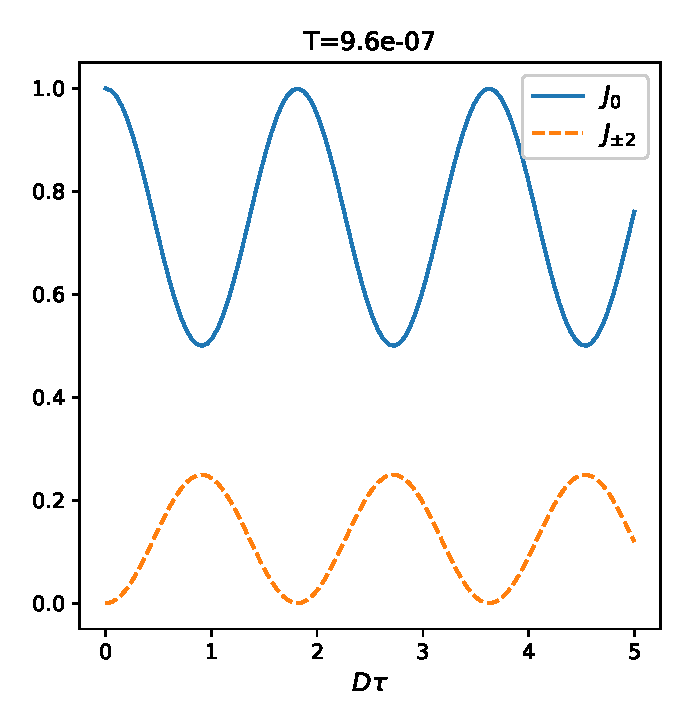
\includegraphics[width=0.5\linewidth]{coherences_n3_beta5.eps}
	\caption{
	  Интенсивности МК~когерентностей~ЯМР~$J_{n}$ ($n=0, 2$) в нанопоре с $N=3$.
      Здесь предполагается, что $\omega_{0} = 2\pi \cdot 500 \cdot 10^{6}$~s$^{-1}$ и $D = 2\pi \cdot 10^{4}$~s$^{-1}$.
	}
	\label{fig:1}
\end{figure}

В этом разделе будет получено точное решение МК~динамики~ЯМР~трехспиновой системы в дипольном упорядоченном состоянии в нанопоре.
Решение будет получена в общем виде, без использования высокотемпературного приближения~\cite{Goldman1970}.
Данная задача аналогична задаче, рассмотренной в разделе~\ref{sec:nanopora-thermodynamic-equilibrium}
для начального термодинамического равновесия в сильном внешнем магнитном поле.

Гамильтониан $H_{MQ}$ уравнения~(\ref{eq:hmq}) состоит из двух блоков для двух возможных значений углового момента спина $(I^2 = S(S+1), \quad S=3/2,1/2)$.
Эти блоки и соответствующие им собственные значения и собственные состояния приведены
в разделе~\ref{sec:sec:nanopora-thermodynamic-equilibrium-exact_sol}.
Матрица плотности системы также состоит из двух блоков $\rho^{3/2}(\tau)$, $\rho^{1/2}(\tau)$, и
%
\begin{equation}
  \label{eq:15}
  \rho^{3/2}(0) = \dfrac 1 Z
  \begin{pmatrix}
    e^{\frac{3b}{2}} & 0 & 0 & 0
    \\
    0 & e^{\frac{-3b}{2}} & 0 & 0
    \\
    0 & 0 & e^{\frac{-3b}{2}} & 0
    \\
    0 & 0 & 0 & e^{\frac{3b}{2}}
  \end{pmatrix},
  \quad
  \rho^{1/2}(0) = \dfrac 1 Z
  \begin{pmatrix}
    	1 & 0
    \\
    0 & 1
  \end{pmatrix}
\end{equation}
%
где $b = \dfrac{\hslash D}{k\mathrm{T}}$ и $T$ --- температура.
Простыми вычислениями можно получить матрицы плотности $\rho^{3/2}(\tau)$ и $\rho^{1/2}(\tau)$,
которые позволяют получить выражение для интенсивности МК~когерентностей~ЯМР.

В рассматриваемых системах появляются только МК~когерентности~ЯМР нулевого и плюс/минус второго порядков.
Интенсивности этих когерентностей равны
%
\begin{equation}
  \begin{split}
    \label{eq:16}
    J_0(\tau) & = 1
    - \dfrac 1 2 \tanh^2\left( \dfrac{3b}{2} \right)
      \sin^2 \left( \sqrt{3} Dt \right),
    \\
    J_{\pm2}(\tau) & = \dfrac{1}{4}
      \tanh^2 \left( \dfrac{3b}{2} \right)
      \sin^2 \left( \sqrt{3} Dt \right)
  \end{split}
\end{equation}
%
Сумма интенсивностей МК когерентностей согласно~(\ref{eq:16}) равна единице в соответствии с уравнением~(\ref{eq:14}).
Зависимости рассчитанных интенсивностей $J_{n}(\tau)$ $(n=0,2)$ от времени эволюции показаны на рисунке~(\ref{fig:1}).

% \subsection{Численный анализ многоспиновой запутанности при различных температурах и различном числе спинов в системе}
\subsection{Температурная зависимость многочастичной запутанности}
\label{sec:5}

В этом разделе приведены результаты полуаналитической симуляции МК эксперимента ЯМР
для модели спин-несущих молекул (атомов) в нанопоре в дипольном упорядоченном состоянии.
Будет рассмотрена зависимость нижней границы квантовой информации Фишера от времени и температуры.
А также получены оценки количества запутанных частиц в системе.
В расчетах предполагается, что $\omega_{0} = 2\pi \cdot 500 \cdot 10^{6}$~s$^{-1}$ и $D = 2\pi \cdot 10^{4}$~s$^{-1}$.

\begin{figure}[H]
 	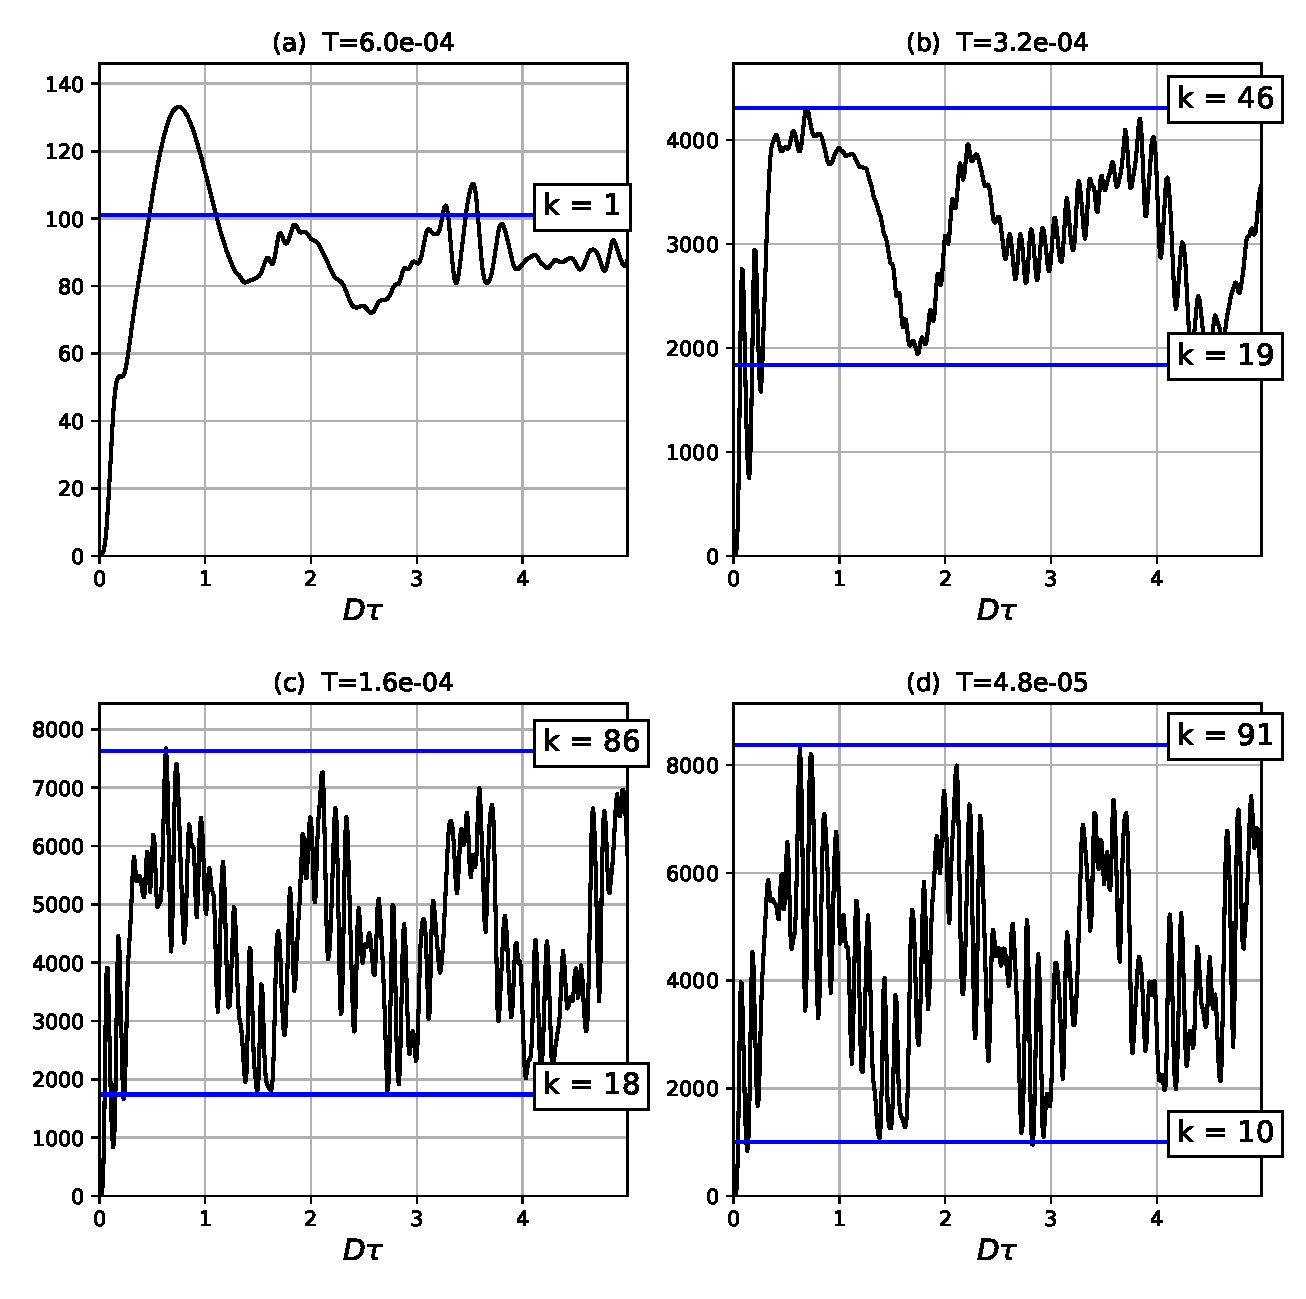
\includegraphics[width=0.95\linewidth]{fisher_low_bound_n101.eps}
	\caption{
	  Зависимость нижней границы  квантовой информации Фишера $F_\mathrm{Q} = 2 M_{2}$
	  от безразмерного времени $D\tau$ при $N=101$.
	  a) $T=6\cdot10^{-4}$~K, неравенство~(\ref{eq:20}) определяет область парной запутанности  (k+1=2), эта область выше горизонтальной линии;
	  b) $T=3.2\cdot10^{-4}$~K, область многоспиновой запутанности представляет собой полосу, ограниченную горизонтальными линиями с~$k=19$~и~$k=46$;
	  c) $T = 1.6\cdot10^{_4}$~K, горизонтальные линии ($k=18$ и $k=86$) ограничивают полосу с многоспиновой запутанностью;
	  d) при $T=4.8\cdot10^{-5}$~K возникают запутанные кластеры с $11-92$ спинами.
	}
	\label{fig:2}
\end{figure}


Рассматриваемая модель спин-несущих молекул (атомов) в нанопоре в дипольном упорядоченном состоянии
расширяет возможности исследования многоспиновой запутанности по сравнению с родственной моделью~(см. раздел~\ref{sec:nanopora-thermodynamic-equilibrium}),
в которой система изначально находилась в термодинамическом равновесии в сильном внешнем магнитном поле.
Модель из раздела~\ref{sec:nanopora-thermodynamic-equilibrium}) неприменима для исследования эволюции системы во времени,
потому что распределение МК~когерентностей~ЯМР~быстро становится стационарным~\cite{Doronin2009}.
Также многоспиновая запутанность изменяется с температурой в очень узком температурном интервале.
Например, все спины запутаны в системе, состоящей из 201 спина уже при температуре $T=6.856\cdot10^{-3}$~K~\cite{Doronin2019}.

Зависимость нижней границы квантовой информации Фишера от времени в системе, состоящей из 101 спина, представлена на Рис.~(\ref{fig:2}) при различных температурах.
Из Рис.~(\ref{fig:2}a) видно, что при температуре $T=6\cdot10^{-4}$~K существует только парная запутанность.
При температуре $T=3.2\cdot10^{-4}$ на Рис.~(\ref{fig:2}b) появляется полоса, в которой неравенство~(\ref{eq:entanglement-criteria}) может быть выполнено, когда $19 \leq k \leq 46$.
Таким образом, существует многоспиновая запутанность в спиновых кластерах, состоящих из 20-47 спинов, при температуре $3.2\cdot10^{-4}$~K.
Когда температура понижается, ширина полосы, в которой существует многоспиновая запутанность, увеличивается.
При температуре $T=1.6\cdot10^{-4}$~K (Рис.~(\ref{fig:2}c)) появляются кластеры из 19-87 запутанных спинов, а при температуре $T=4.8\cdot10^{-5}$~K (Рис.~(\ref{fig:2}d)), наблюдаются 11-92 запутанных спина.

\begin{figure}
 	\includegraphics[width=0.95\linewidth]{entangled_spins_by_n.eps}
	\caption{
	  Зависимость максимального количества запутанных спинов,
	  усредненного по времени эволюции $(0 \leq D\tau \leq 3)$,
	  от температуры при  a) $N=51$; b) $N=75$; c) $N=101$.
	}
	\label{fig:3}
\end{figure}

Зависимость максимального числа запутанных спинов за время эволюции $({0}\leq \mathrm{D}\tau\leq{3})$ от температуры при разных числах спинов в нанопоре представлена на Рис.~(\ref{fig:3}).
Максимальное количество запутанных спинов уменьшается при повышении температуры.
Максимальное количество запутанных спинов увеличивается, когда увеличивается число спинов в нанопоре, потому что система в нанопоре становится плотнее.

\section{Выводы}
\label{sec:conslusions}
% We investigated many-particle entanglement in MQ NMR spectroscopy using a nanocavity filled with spin-carrying atoms (molecules).
% We developed a theory of MQ NMR in a nanocavity at low temperatures.
% The theory is based on the idea that  molecular diffusion is substantially faster than the time of the spin flip-flop processes.
% As a result, the problem is reduced to a system of equivalent spins [23, 25], which can be analyzed in the basis of the common eigenstates of the total spin angular momentum and its projection on the external magnetic field.
% Since there is a connection between the second moment (dispersion) of the distribution of the MQ NMR intensities and many-spin entanglement [17], we extracted information about many-spin entanglement from the MQ NMR spectrum. The temperature dependence of many-spin entanglement was also investigated.
% \par
% The main lesson consists in significant growth of many-particle entanglement at low temperatures.
% All or almost all spins are entangled at the dimensionless temperature $\frac{1}{b}$ of the order of 1.
% This suggests that $k$-entangled states with large $k$ emerge in a typical MQ NMR system at low temperatures.
% This is particularly interesting given the absence of entanglement in the initial state. We expect such behavior to be typical for MQ NMR.
% \par
% We can conclude that MQ NMR spectroscopy is an effective method for the investigation of many-spin entanglement and the spreading of MQ correlations inside many-spin systems. It can be used for experimental investigations of quantum information processing in solids (note a related study of decoherence in liquids \cite{HOU2017863}).
% \par

В этой главе была исследована многочастичная запутанность в МК спектроскопии ЯМР в нанопоре, заполненной сотнями спин-несущими частицами.
Для этого была разработана МК теория ЯМР в нанопоре при низких температурах.
Было рассмотрено два начальных состояния системы:
термодинамически равновесное
и дипольное упорядоченное.
В обоих случах впервые удалось исследовать температурную зависимость многочастичной запутанности.
Все или почти все спины запутаны при безразмерной температуре $\frac{1}{b}$ порядка 1.
Это говорит о том, что $k$-запутанные состояния с большим $k$ возникают в типичной системе МК ЯМР при низких температурах.
Это особенно интересно, учитывая отсутствие запутанности в начальном состоянии.
Можно заключить, что такое поведение типично для МК ЯМР.
Так же была исследована зависимость многоспиновой запутанности
от количества спинов в нанопоре.
Показано, что с ростом количества спинов в нанопоре,
скорость возникновения запутанных кластеров при понижении температуры увеличивается.

Результаты этого раздела наглядно демонстрируют
универсальность разработанного в этой диссертации метода исследования многочастичной запутанности.

\begin{frame}{Эволюция нижней границы информации Фишера}
% (AMR-20)\footnote{G.A. Bochkin et al., \textit{Appl. Magn. Res.} \textbf{51}, 667-678, (2020)}
\begin{columns}

    \column{0.6\textwidth}
    \begin{figure}
    
\includegraphics[width=0.95\textwidth]{result-zchain-m2-by-time-n6-beta10.eps}
    %\caption{Hанопора со спин-несущих молекулами во внешнем сильном магнитном поле $\vec B$}
    \end{figure}

    \column{0.4\textwidth}
    Зависимость нижней границы квантовой информации Фишера
    $$ F_Q = 2M_2(\tau, T) $$
    от безразмерного времени $D_1 \tau$
    для шести спинов
    при температуре $T = 2.5 \times 10^{-3}$ $(\beta = 10)$.
    Область многочастичной запутанности ограничена горизонтальными линиями $k = 1$, $k = 5$.
\end{columns}
\end{frame}
\note{
   Мы не можем точно сказать сколько спинов запутанно,
   но можем дать нижнюю оценку на количество запутанных между собой спинов.
}


\begin{frame}{Максимальное количество запутанных спинов}
\begin{columns}

    \column{0.5\textwidth}
    \begin{figure}
    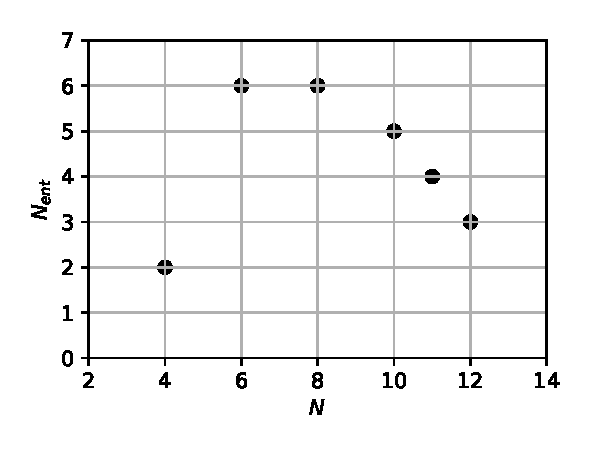
\includegraphics[width=\textwidth]{result-zchain-nent-by-n-beta10.eps}
    \caption{}
    \end{figure}

    \column{0.5\textwidth}
    Зависимость максимального количества запутанных спинов $N_\mathrm{ent}$ от длины цепи при температуре $T = 2.5 \times 10^{-3}$ $(\beta = 10)$.

    \vspace{0.5cm}

    \alert{Создание запутанных кластеров в рассматриваемых зигзагообразных цепочках ограничено слабыми дипольными взаимодействиями удаленных спинов}.
\end{columns}
\end{frame}
\note{
  Установлено что, при фиксированной температуре с ростом числа спинов в цепи размер запутанных кластеров может уменьшаться;
}


\begin{frame}{Максимальное количество запутанных спинов}
  \begin{columns}
     \column{0.5\textwidth}
     \begin{figure}
     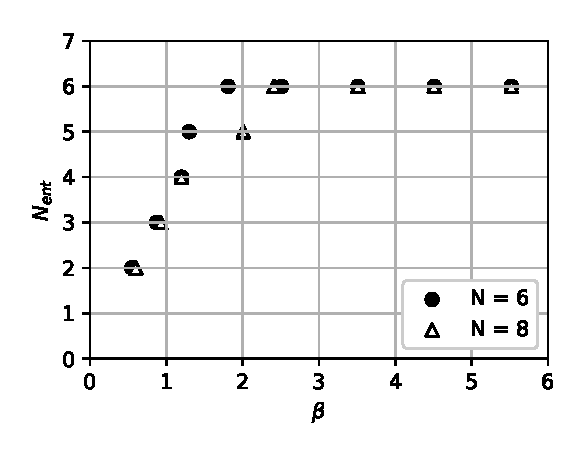
\includegraphics[width=\textwidth]{result-zchain-nent-by-beta-n8-n6.eps}
     \caption{}
     \end{figure}

     \column{0.45\textwidth}
     \begin{block}{}
       Зависимость максимального количества запутанных спинов $N_\mathrm{ent}$ от обратной температуры
       $$ \beta = \dfrac{\hbar\omega_0}{kT} $$
       в зигзагообразной цепочки из 6 и 8 спинов.
    \end{block}
  \end{columns}
\end{frame}
\note{
    Для 6 спинов накачка происходит быстрее, чем для 8 спинов.
}

\chapter{Измерение информации Вигнера-Янасе в МК эксперименте ЯМР}
\label{chapter:wyi-mesuarement}

% PLA-2021
\item
Разработана теория МК ЯМР в системе эквивалентных спинов s=1/2 при произвольных температурах. При низких температурах эта теория применена для расчетов многоспиновой запутанности в
нанопоре и зигзагообразной цепочке. 
Проведенные исследования позволяют заключить, что МК-спектроскопия ЯМР является тонким и полезным методом для исследования различных проблем квантовой информатики.

\item
Исследована температурная зависимость многочастичной запутанности в нанопоре с термодинамическим равновесным зеемановским и дипольно упорядоченным начальными состояниями. 
С понижением температуры количество запутанных спинов растет.
При температуре
$T = 6.856\cdot10^{-3}$~K $(\beta=3.5)$
почти все спины (до 179 из 201) запутаны. 
Можно заключить, что в типичной системе МК ЯМР при низких температурах возникают многочастичные запутанные состояния,
даже при отсутствии запутанности в начальном состоянии.  


\item
Исследована многочастичная запутанность в квазиодномерных цепочках ядерных спинов в зависимости от параметров цепи и температуры.
В однородных цепочках детектируется только парная запутанность, что согласуется с результатами, представленными в литературе.
В зигзагообразной цепочке при низких температурах почти все спины запутанны, так же как и в нанопоре.

\item
Предложен метод экспериментального измерения точного значения косой информации Вигнера-Янасе в рамках МК спектроскопии ЯМР.
Разработанный метод позволяет не только исследовать многочастичную запутанность методами МК ЯМР,
но и открывает возможность решения широкого класса задач квантовой теории информации.


\begin{thebibliography}{}

\bibitem{Einstein1935} A. Einstein, B. Podolsky, and N. Rosen \textit{Phys. Rev.} \textbf{47}, 777 (1935)
\bibitem{Bell1964} J.S. Bell \textit{Physics Physique Fizika} \textbf{1}, 195 (1964)
\bibitem{Scheidl2010} T. Scheidl et al. \textit{PNAS} \textbf{107}, 46, 19708-19713 (2010)

\bibitem{Bernabeu2012} Bernabéu, J., Martínez-Vidal, F. and Villanueva-Pérez, P. J. High Energ. Phys. 2012, 64 (2012).

\bibitem{Alain1976} Alain Aspect Phys. Rev. D 14, 1944 – Published 15 October 1976

% Zeqian Chen Phys. Rev. A 71, 052302
\bibitem{Gisin1991} N. Gisin, Phys. Lett. A 154, 201 (1991).
\bibitem{Clauser1969} J. F. Clauser, M. A. Horne, A. Shimony, and R. A. Holt, Phys. Rev. Lett. 23, 880 (1969).
\bibitem{Seevinck2002} M. Seevinck and G. Svetlichny, ibid. 89, 060401 (2002).
\bibitem{Uffink2002}  J. Uffink, Phys. Rev. Lett. 88, 230406 (2002O); K. Nagata, M. Koashi, and N. Imoto, ibid. 89, 260401 (2002).
%

\bibitem{Bennett1996} C.H.Bennett et al. \textit{Phys. Rev. A} \textbf{54}, 3824 (1996)
\bibitem{Eisert2001} Eisert J. and Briegel H. J. \textit{Phys. Rev. A} \textbf{64}, 022306 (2001)
\bibitem{Wootters1998} W.K. Wootters, \textit{Phys. Rev. Lett.} \textbf{80}, 2245 (1998)


% [5 - 31] P. Hyllus et al. Phys. Rev. A 85, 022321 (2012)
\bibitem{Plenio2007} M.B. Plenio and S. Virmani, Quant. Inf. Comp. 7, 1 (2007).
\bibitem{Amico2008} L. Amico, R. Fazio, A. Osterloh, and V. Vedral, Rev. Mod. Phys. 80, 517 (2008).
\bibitem{Horodecki2009} R. Horodecki, P. Horodecki, M. Horodecki, and K. Horodecki, Rev. Mod. Phys. 81, 865 (2009).
\bibitem{Guhne2009} O. G\"uhne and G. Toth, Physics Reports 474, 1 (2009).
\bibitem{Bourennane2004} M. Bourennane, M. Eibl, C. Kurtsiefer, S. Gaertner, H. Weinfurter, O. G\"uhne, P. Hyllus, D. Bruß, M. Lewenstein, and A. Sanpera, Phys. Rev. Lett. 92, 087902
\bibitem{Kaszlikowski2008} D. Kaszlikowski and A. Kay, New. J. Phys. 10, 053026 (2008).
\bibitem{Krammer2009} P. Krammer, H. Kampermann, D. Bruß, R.A. Bertlmann, L.C. Kwek, C. Macchiavello, Phys. Rev. Lett. 103, 100502 (2009).
\bibitem{Bancal2011} J.-D. Bancal, N. Gisin, Y.-C. Liang, and S. Pironio, PRL 106, 250404 (2011).
\bibitem{Svetlichny1987} G. Svetlichny, Phys. Rev. D 35, 3066 (1987).
\bibitem{Gisin1998} N. Gisin and H. Bechmann-Pasquinucci, Phys. Lett. A 246, 1 (1998).
\bibitem{Collins2002} D. Collins, N. Gisin, S. Popescu, D. Roberts, and V. Scarani, Phys. Rev. Lett. 88, 170405 (2002).
\bibitem{Seevinck2001} M. Seevinck and J. Uffink, Phys. Rev. A 65, 012107 (2001);
\bibitem{Toth2005} G. T\'oth, O. G\"uhne, M. Seevinck, and J. Uffink, Phys. Rev. A 72, 014101 (2005).
\bibitem{Nagata2002} K. Nagata, M. Koashi, and N. Imoto, Phys. Rev. Lett. 89, 260401 (2002).
\bibitem{Yu2003} S. Yu, Z.-B. Chen, J.-W. Pan, and Y.-D. Zhang, Phys. Rev. Lett. 90, 080401 (2003)
\bibitem{Laskowski2005} W.Laskowski and M.Zukowski, Phys.Rev.A72, 062112 (2005).
\bibitem{Schmid2008} C. Schmid, N. Kiesel, W. Laskowski, W. Wieczorek, and M.Z\'ukowski,and H.Weinfurter,Phys.Rev.Lett.100, 200407 (2008).
\bibitem{Bancal2009} J.-D. Bancal, C. Branciard, N. Gisin, and S. Pironio, Phys. Rev. Lett. 103, 090503 (2009).
\bibitem{Sorensen2001} A.S. Sørensen and K. Mølmer, Phys. Rev. Lett. 86, 4431 (2001).
\bibitem{Durkin2005} G.A. Durkin and C. Simon, Phys. Rev. Lett. 95, 180402 (2005).
\bibitem{Vitagliano2011} G. Vitagliano, P. Hyllus, I.L. Egusquiza, G. T\'oth, Phys. Rev. Lett. 107, 240502 (2011).
\bibitem{Duan2011} L.-M. Duan, Phys. Rev. Lett. 107, 180502 (2011).
\bibitem{Guhne2010} O. Guhne and M. Seevinck, New J. Phys. 12, 053002 (2010).
\bibitem{Huber2010} M. Huber, F. Mintert, A. Gabriel, and B.C. Hiesmayr, Phys. Rev. Lett. 104, 210501 (2010).
\bibitem{Li2010} C.-M. Li, K. Chen, A. Reingruber, Y.N. Chen, and J.W. Pan, Phys. Rev. Lett. 105, 210504 (2010).
\bibitem{Jungnitsch2011} B. Jungnitsch, T. Moroder, and O. G\"uhne, Phys. Rev. Lett. 106, 190502 (2011).
\bibitem{Vicente2011} J.I. de Vicente and M. Huber, Phys. Rev. A 84, 062306 (2011).
\bibitem{Huber2011} M. Huber, P. Erker, H. Schimpf, A. Gabriel, and B. Hiesmayr, Phys. Rev. A 83, 040301(R) (2011).
%---


\bibitem{Zeqian2005} Zeqian Chen \textit{Phys. Rev. A} \textbf{71}, 052302 (2005)

\bibitem{Hyllus2012} P. Hyllus et al. \textit{Phys. Rev. A} \textbf{85}, 022321 (2012)


% [19] Phys. Rev. A 71, 052302 (2005)
\bibitem{Wheeler2004} J.Wheeler, in Complexity, Entropy, and Physics of Information, edited by Z.H.Zurek (Addison-Wesley, Reading, MA, 1990), pp.3-28;
\bibitem{Summhammer2004}
J.Summhammer, Int.J.Theor.Phys. 33, 171(1994);
\bibitem{Frieden2004} B.R.Frieden, Science from Fisher Information: A Unification(Cambridge University Press, Cambridge, England, 2004).

\bibitem{khitrin1997} A. Khitrin, Chem. Phys. Lett. 274, 217 (1997)

\bibitem{g_arttner2018} M. G\"arttner, P. Hauke, and A. M. Rey, Phys. Rev. Lett. 120, 040402 (2018)

\bibitem{t_oth2014} G. T\"oth and I. Apellaniz, J. Phys. A 47, 424006 (2014)

\bibitem{pezz_e2018} L. Pezz\'e, A. Smerzi, M. K. Oberthaler et al., Rev. Mod. Phys. 90, 035005 (2018).

\bibitem{liu2014} J. Liu, H.-N. Xiong, F. Song, and X. Wang, Physica A 410, 167 (20


% Quatntum Fisher Information
\bibitem{Helstrom1976} C. W. Helstrom, Quantum detection and estimation theory, Academic Press, New York, 1976.
\bibitem{Holevo1982} A. S. Holevo, Probabilistic and statistical aspects of quantum theory, North-Holland, Amsterdam, 1982.


% Wigner yanase

% 10.1103/PhysRevLett.91.180403
% [3]
\bibitem{Araki1961} H. Araki and M. M. Yanase, Phys. Rev. 120, 622 (1960). [4] M. M. Yanase, Phys. Rev. 123, 666 (1961).
% [5]
\bibitem{Ozawa1991} M. Ozawa, Phys. Rev. Lett. 67, 1956 (1991).
% [6]
\bibitem{Ozawa2002a} M. Ozawa, Phys. Rev. Lett. 88, 050402 (2002).
% [7]
\bibitem{Ozawa2002b} M. Ozawa, Phys. Rev. Lett. 89, 057902 (2002).
% [8]
\bibitem{Matsumoto1993} S. Matsumoto, Prog. Theor. Phys. 90, 35 (1993).
% [9]
\bibitem{Kakazu3469} K. Kakazu and S. Pascazio, Phys. Rev. A 51, 3469
(1995).

% Chen2005
% 10.1103/PhysRevA.71.052302
% 3
% \bibitem{Einstein1935} A. Einstein, B. Podolsky, and N. Rosen, Phys. Rev. 47, 777 (1935).
% % 4
% \bibitem{Gisin1991} N. Gisin, Phys. Lett. A 154, 201 (1991).
% % 5
% \bibitem{Clauser1969} J. F. Clauser, M. A. Horne, A. Shimony, and R. A. Holt, Phys. Rev. Lett. 23, 880 (1969).
% ��6�� D. Collins, N. Gisin, S. Popescu, D. Roberts, and V. Scarani,
% Phys. Rev. Lett. 88, 170405 ��2002��; M. Seevinck and G.
% Svetlichny, ibid. 89, 060401 ��2002��.
% ��7�� J. Uffink, Phys. Rev. Lett. 88, 230406 ��2002��; K. Nagata, M.
% Koashi, and N. Imoto, ibid. 89, 260401 ��2002��.
% ��8�� S.-X. Yu, Z.-B. Chen, J.-W. Pan, and Y.-D. Zhang, Phys. Rev.
% Lett. 90, 080401 ��2003��.
% ��9�� E. P. Wigner, Z. Phys. 133, 101 ��1952��; Physikertagung Wien
% ��Physik-Verlag, Mosbach, 1952��, p. 1.

% E. P. Wigner and M. M. Yanase, \textit{Proc. Nat. Acad. Sci. USA}, \textbf{49}, 910–918 (1963)
% [1]
\bibitem{Weaver1949} W. Weaver's article in The Mathematical Theory of Communication (Urbana: The University of IllinoisPress,1949),p.45. SeealsothelastfewpagesofM.v.Smoluchowski'sarticleinVortrage fiberdie kinetische Theorie der Materie und Elektrizit4t (Leipzig: B. G. Teubner, 1914).
% [2]
\bibitem{Wigner1960} Wigner, E. P., Z. Physik, 131, 101 (1952); Araki, H., and M. M. Yanase, Phys. Rev., 120, 622(1960).
% [3]
\bibitem{Wigner1962} Wigner,E.P.,PhysikertagungWien(Mosbach/Baden: PhysikVerlag,1962),p.1

\bibitem{Wigner1963} E. P. Wigner and M. M. Yanase, \textit{Proc. Nat. Acad. Sci. USA}, \textbf{49}, 910–918 (1963) https://www.pnas.org/doi/abs/10.1073/pnas.49.6.910

\bibitem{Luo2003} S. Luo, \textit{Phys. Rev. Lett.} \textbf{91}, 180403 (2003)

\bibitem{Lieb1973prl} E. H. Lieb and M. B. Ruskai, “A fundamental property of quantum-mechanical entropy,” Phys. Rev. Lett., 30, 434–436 (1973).
\bibitem{Lieb1973} E. H. Lieb, “Convex trace functions and the Wigner–Yanase–Dyson conjecture,” Adv. Math., 11, 267–288 (1973).
\bibitem{Wehrl1978} A. Wehrl, “General properties of entropy,” Rev. Modern Phys., 50, 221–260 (1978).

\bibitem{Luo2005} S. L. Luo, “Quantum versus classical uncertainty,” Theor. Math. Phys., 143, 681–688 (2005).
\bibitem{Luo2005pra} S. Luo, “Heisenberg uncertainty relation for mixed states,” Phys. Rev. A, 72, 042110 (2005).
\bibitem{Luo2006} S. Luo, “Quantum uncertainty of mixed states based on skew information,” Phys. Rev. A, 73, 022324 (2006).
\bibitem{Luo2017pra} S. Luo and Y. Sun, “Quantum coherence versus quantum uncertainty,” Phys. Rev. A, 96, 022130 (2017).

\bibitem{Luo2020} S. Luo, Theoretical and Mathematical Physics, 202(1): 104–111 (2020)
% [9-23] Luo, Theoretical and Mathematical Physics, 202(1): 104–111 (2020)
% 9.
\bibitem{Luo2012} S. Luo, S. Fu, and C. H. Oh, “Quantifying correlations via the Wigner–Yanase skew information,” Phys. Rev. A,
85, 032117 (2012).
%10.
\bibitem{Li2016a} L. Li, Q.-W. Wang, S.-Q. Shen, and M. Li, “Measurement-induced nonlocality based on Wigner–Yanase skew
information,” Europhys. Lett., 114, 10007 (2016).
%11.
\bibitem{Sun2017} Y. Sun, Y. Mao, and S. Luo, “From quantum coherence to quantum correlations,” Europhys. Lett., 118, 60007
(2017).
% 12.
\bibitem{Girolami2014} D. Girolami, “Observable measure of quantum coherence in finite dimensional systems,” Phys. Rev. Lett., 113,
170401 (2014); arXiv:1403.2446v3 [quant-ph] (2014).
% 13.
\bibitem{Yu2017} C. Yu, “Quantum coherence via skew information and its polygamy,” Phys. Rev. A, 95, 042337 (2017); arXiv:
1704.04871v1 [quant-ph] (2017).
% 14.
\bibitem{Luo2017} S. Luo and Y. Sun, “Partial coherence with application to the monotonicity problem of coherence involving skew
information,” Phys. Rev. A, 96, 022136 (2017).
% 15.
\bibitem{Luo2018} S. Luo and Y. Sun, “Coherence and complementarity in state-channel interaction,” Phys. Rev. A, 98, 012113
(2018).
% 16.
\bibitem{Karpat2014} G. Karpat, B. Cakmak, and F. F. Fanchini, “Quantum coherence and uncertainty in the anisotropic XY chain,”
Phys. Rev. B, 90, 104431 (2014); arXiv:1404.6427v3 [quant-ph] (2014).
% 17.
\bibitem{Malvezzi2016} A. L. Malvezzi, G. Karpat, B. Cakmak, F. F. Fanchini, T. Debarba, and R. O. Vianna, “Quantum correlations
and coherence in spin-1 Heisenberg chains,” Phys. Rev. B, 93, 184428 (2016); arXiv:1602.03731v2 [quant-ph]
(2016).
% 18.
\bibitem{Li2016b} Y.-C. Li and H.-Q. Lin, “Quantum coherence and quantum phase transitions,” Sci. Rep., 6, 26365 (2016).
% 19.
\bibitem{Lei2016} S. Lei and P. Tong, “Wigner–Yanase skew information and quantum phase transition in one-dimensional quantum spin-1/2 chains,” Quantum Inf. Process., 15, 1811–1825 (2016).
% 20.
\bibitem{Qiu2017} L. Qiu, D. Quan, F. Pan, and Z. Liu, “Skew information in the XY model with staggered Dzyaloshinskii–Moriya
interaction,” Phys. B, 514, 13–18 (2017).
% 21.
\bibitem{Yanagi2005} K. Yanagi, S. Furuichi, and K. Kuriyama, “A generalized skew information and uncertainty relation,” IEEE Trans. Inform. Theory, 51, 4401–4404 (2005).
% 22.
\bibitem{Furuichi2010} S. Furuichi, “Schrodinger uncertainty relation with Wigner–Yanase skew information,” Phys. Rev. A, 82, 034101 (2010); arXiv:1005.2655v2 [quant-ph] (2010).
% 23.
\bibitem{Chen2016} B. Chen, S.-M. Fei, and G.-L. Long, “Sum uncertainty relations based on Wigner–Yanase skew information,” Quantum Inf. Process., 15, 2639–2648 (2016); arXiv:1606.01533v1 [quant-ph] (2016).
/Furuichi2010


% mq expreimetn
\bibitem{Baum1985} J. Baum, M. Munowitz, A. N. Garroway, and A. Pines, J. Chem. Phys. 83, 2015 (1985).


% models
\bibitem{Baugh2001}J. Baugh, A. Kleinhammes, D. Han, Q. Wang, and Y. Wu, \textit{Science} \textbf{294}, 1505 (2001).


% MQ NMR

%% Master diploma
\bibitem{vesta} Koichi Momma and Fujio Izumi. VESTA 3 for three-dimensional visualization of crystal, volumetric and morphology data. Journal of Applied Crystallography, 44(6):1272–1276, Dec 2011.

\bibitem{Elliott1994} J. C. Elliott. Structure and chemistry of the apatites and other calcium orthophosphates. Studies in Inorganic Chemistry 18. Elsevier Science, Amsterdam, 1994.

%% JETP Lett. 2015
%\bibitem{Baum1985} J. Baum, M. Munoviz, A. N. Garroway, and A. Pines. Multiple quantum dynamics in solid state NMR. The Journal of Chemical Physics, 83(5):2015– 2025, 1985.

%%
\bibitem{Bochkin2019jmr} G.A. Bochkin, E.B. Fel’dman, I.D. Lazarev, A.A. Samoilenko, S.G. Vasil’ev, Orientational dependencies of dynamics and relaxation of multiple quantum NMR coherences in one-dimensional systems, Journal of Magnetic Resonance (2019), doi: https://doi.org/10.1016/j.jmr.2019.02.004

%% JMR 2020
% []
% [1]
% \bibitem{Baum1985} J. Baum, M. Munowitz, A.N. Garroway, A. Pines, J. Chem. Phys. 83 (5) (1985) 2015–2025.
% [2]
\bibitem{Hughes2004} C.E. Hughes, Prog. Nucl. Magn. Reson. Spectrosc. 45 (3–4) (2004) 301–313.
% [3]
\bibitem{Vasilev2018} S.G. Vasil’ev, V.I. Volkov, E.A. Tatarinova, A.M. Muzafarov, N.A. Sipyagina, S.A. Lermontov, J. Non-Cryst. Solids 489 (2018) 6–15.
% [4]
\bibitem{Avilova2019} I.A. Avilova, A.V. Chernyak, S.G. Vasil’ev, Appl. Magn. Resonan. 50 (12) (2019) 1419 –1428.
% [5]
\bibitem{Mogami2014} Y. Mogami, S. Yamazaki, S. Matsuno, K. Matsui, Y. Noda, K. Takegoshi, Cem. Concr. Res. 66 (2014) 115–120.
% [6]
\bibitem{Krojanski2006} H.G. Krojanski, D. Suter, Phys. Rev. A 74 (6) (2006) 062319.
% [7]
\bibitem{Cho2006} H. Cho, P. Cappellaro, D.G. Cory, C. Ramanathan, Phys. Rev. B 74 (22) (2006) 224434.
% [8]
\bibitem{Bochkin2018} G.A. Bochkin, E.B. Fel’dman, S.G. Vasil’ev, V.I. Volkov, Appl. Magn. Reson. 49 (1) (2018) 25–34.
% [9]
\bibitem{Sanchez2014} C.M. S\'anchez, R.H. Acosta, P.R. Levstein, H.M. Pastawski, A.K. Chattah, Phys. Rev. A 90 (4) (2014) 042122.
% [10]
\bibitem{Alvarez2015} G.A. \'Alvarez, D. Suter, R. Kaiser, Science 349 (6250) (2015) 846–848.
% [11]
\bibitem{Wei2018} K.X. Wei, C. Ramanathan, P. Cappellaro, Phys. Rev. Lett. 120 (7) (2018) 070501.
% [12]
\bibitem{Garttner2018} M. G\"arttner, P. Hauke, A.M. Rey, Phys. Rev. Lett. 120 (4) (2018) 040402.
% [13]
\bibitem{Doronin2019} S.I. Doronin, E.B. Fel’dman, I.D. Lazarev, Phys. Rev. A 100 (2) (2019) 022330.
% [14]
\bibitem{Starkov2020}  G.A. Starkov, B.V. Fine, Phys. Rev. B 101 (2) (2020) 024428.
% [15]
\bibitem{Zhang2009} W. Zhang, P. Cappellaro, N. Antler, B. Pepper, D.G. Cory, V.V. Dobrovitski, C. Ramanathan, L. Viola, Phys. Rev. A 80 (5) (2009) 052323.
% [16]
\bibitem{Feldman2014} E.B. Fel’dman, Appl. Magn. Reson. 45 (8) (2014) 797–806.
% [17]
\bibitem{Feldman1997} E.B. Fel’dman, S. Lacelle, J. Chem. Phys. 107 (18) (1997) 7067–7084.
% [18]
\bibitem{Hayashi1960} S. Hayashi, Nippon kagaku zassi 81 (4) (1960) 540–542.
% [19]
\bibitem{Van1964} W. Van der Lugt, W.J. Caspers, Physica 30 (8) (1964) 1658–1666.
% [20]
\bibitem{ChoCho} G. Cho, J.P. Yesinowski, J. Phys. Chem. 100 (39) (Cho) 15716–15725.
% [21]
\bibitem{Itoh2005} K.M. Itoh, Solid State Commun. 133 (11) (2005) 747–752.
% [22]
\bibitem{Zachariasen1931} W.H. Zachariasen, Zeitschrift für Kristallographie - Crystalline Materials 76 (1) (1931) 289–302.
% [23]
\bibitem{Zachariasen1963} W.H. Zachariasen, H.A. Plettinger, M. Marezio, Acta Crystallogr. A 16 (11) (1963) 1144–1146.
% [24]
\bibitem{Gatta2012} G.D. Gatta, J.M. Garry, B. Geoffrey, G. Alessandro, N. Fabrizio, Am. Mineral. 97 (11–12) (2012) 1891–1897.
% [25]
\bibitem{Burns1995} P.C. Burns, M. Novak, F.C. Hawthorne, Can. Mineralogist 33 (6) (1995) 1205– 1213.
% [26]
\bibitem{Bochkin2019} G.A. Bochkin, E.B. Fel’dman, I.D. Lazarev, A.A. Samoilenko, S.G. Vasil’ev, J. Magn. Reson. 301 (2019) 10–18.
% [27]
\bibitem{Abragam1961} A. Abragam, The principles of nuclear magnetism, Clarendon Press, Oxford, 1961.
% [28]
\bibitem{Carolan1971} J.L. Carolan, Chem. Phys. Lett. 12 (2) (1971) 389–391.
% [29]
\bibitem{Vleck1948} J.H. Van Vleck, Phys. Rev. 74 (9) (1948) 1168–1183.
% [30]
\bibitem{Engelsberg1973} M. Engelsberg, I.J. Lowe, J.L. Carolan, Phys. Rev. B 7 (3) (1973) 924–929.
%% --


\end{thebibliography}


\end{document}